\documentclass[a4paper,12pt,twoside]{memoir}

% Castellano
\usepackage[spanish,es-tabla]{babel}
\selectlanguage{spanish}
\usepackage[utf8]{inputenc}
\usepackage[T1]{fontenc}
\usepackage{lmodern} % scalable font
\usepackage{microtype}
\usepackage{placeins}

\RequirePackage{booktabs}
\RequirePackage[table]{xcolor}
\RequirePackage{xtab}
\RequirePackage{multirow}

\RequirePackage{todonotes}

% Añado listings para ver el código en la memoria mejor
\usepackage{listings}

% Links
\PassOptionsToPackage{hyphens}{url}\usepackage[colorlinks]{hyperref}
\hypersetup{
	allcolors = {red}
}

% Acrónimos
\usepackage[acronym]{glossaries}
\makenoidxglossaries

\newacronym{llm}{LLM}{\textit{Large Language Models}}
\newacronym{ods}{ODS}{\textit{Objetivos de Desarrollo Sostenible}}
\newacronym{ods11}{ODS11}{\textit{Ciudades y Comunidades Sostenibles}}
\newacronym{sdg}{SDG}{\textit{Sustainable Development Goals}}
\newacronym{sc}{Smart City}{\textit{Ciudades Inteligentes}}
\newacronym{sdg11}{SDG11}{\textit{Sustainable Cities and Communities}}
\newacronym{pdi}{PDI}{\textit{Punto de Interés}}
\newacronym{tfg}{TFG}{\textit{Trabajo de Fin de Grado}}
\newacronym{so}{SO}{\textit{Sistema Operativo}}
\newacronym{gps}{GPS}{\textit{Global Positioning System}}
\newacronym{sig}{GIS}{\textit{Sistemas de Información Geográfica}}
\newacronym{bloc}{BLoC}{\textit{Business Logic Component}}
\newacronym{ia}{IA}{\textit{Inteligencia Artificial}}

\newglossaryentry{eco-city-tour}
{
	name=Eco City Tour,
	description={es una ruta turística compuesta por Puntos de Interés Turístico (PDI)}
}

\newcommand{\autor}{Fernando Pisot Serrano}

% Ecuaciones
\usepackage{amsmath}

% Rutas de fichero / paquete
\newcommand{\ruta}[1]{{\sffamily #1}}

% Párrafos
\nonzeroparskip

% Huérfanas y viudas
\widowpenalty100000
\clubpenalty100000

% Evitar solapes en el header
\nouppercaseheads

% Imagenes
\usepackage{graphicx}
\newcommand{\imagen}[2]{
	\begin{figure}[!h]
		\centering
		\includegraphics[width=0.9\textwidth]{#1}
		\caption{#2}\label{fig:#1}
	\end{figure}
	\FloatBarrier
	
}

\newcommand{\imagenflotante}[2]{
	\begin{figure}%[!h]
		\centering
		\includegraphics[width=0.9\textwidth]{#1}
		\caption{#2}\label{fig:#1}
	\end{figure}
}

\newcommand{\imagenminipage}[2]{
	\centering
	\includegraphics[width=0.9\textwidth]{#1}
	\textbf{Figura:} #2
}



% El comando \figura nos permite insertar figuras comodamente, y utilizando
% siempre el mismo formato. Los parametros son:
% 1 -> Porcentaje del ancho de página que ocupará la figura (de 0 a 1)
% 2 --> Fichero de la imagen
% 3 --> Texto a pie de imagen
% 4 --> Etiqueta (label) para referencias
% 5 --> Opciones que queramos pasarle al \includegraphics
% 6 --> Opciones de posicionamiento a pasarle a \begin{figure}
\newcommand{\figuraConPosicion}[6]{%
  \setlength{\anchoFloat}{#1\textwidth}%
  \addtolength{\anchoFloat}{-4\fboxsep}%
  \setlength{\anchoFigura}{\anchoFloat}%
  \begin{figure}[#6]
    \begin{center}%
      \Ovalbox{%
        \begin{minipage}{\anchoFloat}%
          \begin{center}%
            \includegraphics[width=\anchoFigura,#5]{#2}%
            \caption{#3}%
            \label{#4}%
          \end{center}%
        \end{minipage}
      }%
    \end{center}%
  \end{figure}%
}

%
% Comando para incluir imágenes en formato apaisado (sin marco).
\newcommand{\figuraApaisadaSinMarco}[5]{%
  \begin{figure}%
    \begin{center}%
    \includegraphics[angle=90,height=#1\textheight,#5]{#2}%
    \caption{#3}%
    \label{#4}%
    \end{center}%
  \end{figure}%
}
% Para las tablas
\newcommand{\otoprule}{\midrule [\heavyrulewidth]}
%
% Nuevo comando para tablas pequeñas (menos de una página).
\newcommand{\tablaSmall}[5]{%
 \begin{table}
  \begin{center}
   \rowcolors {2}{gray!35}{}
   \begin{tabular}{#2}
    \toprule
    #4
    \otoprule
    #5
    \bottomrule
   \end{tabular}
   \caption{#1}
   \label{tabla:#3}
  \end{center}
 \end{table}
}

%
%Para el float H de tablaSmallSinColores
\usepackage{float}

%
% Nuevo comando para tablas pequeñas (menos de una página).
\newcommand{\tablaSmallSinColores}[5]{%
 \begin{table}[H]
  \begin{center}
   \begin{tabular}{#2}
    \toprule
    #4
    \otoprule
    #5
    \bottomrule
   \end{tabular}
   \caption{#1}
   \label{tabla:#3}
  \end{center}
 \end{table}
}

\newcommand{\tablaApaisadaSmall}[5]{%
\begin{landscape}
  \begin{table}
   \begin{center}
    \rowcolors {2}{gray!35}{}
    \begin{tabular}{#2}
     \toprule
     #4
     \otoprule
     #5
     \bottomrule
    \end{tabular}
    \caption{#1}
    \label{tabla:#3}
   \end{center}
  \end{table}
\end{landscape}
}

%
% Nuevo comando para tablas grandes con cabecera y filas alternas coloreadas en gris.
\newcommand{\tabla}[6]{%
  \begin{center}
    \tablefirsthead{
      \toprule
      #5
      \otoprule
    }
    \tablehead{
      \multicolumn{#3}{l}{\small\sl continúa desde la página anterior}\\
      \toprule
      #5
      \otoprule
    }
    \tabletail{
      \hline
      \multicolumn{#3}{r}{\small\sl continúa en la página siguiente}\\
    }
    \tablelasttail{
      \hline
    }
    \bottomcaption{#1}
    \rowcolors {2}{gray!35}{}
    \begin{xtabular}{#2}
      #6
      \bottomrule
    \end{xtabular}
    \label{tabla:#4}
  \end{center}
}

%
% Nuevo comando para tablas grandes con cabecera.
\newcommand{\tablaSinColores}[6]{%
  \begin{center}
    \tablefirsthead{
      \toprule
      #5
      \otoprule
    }
    \tablehead{
      \multicolumn{#3}{l}{\small\sl continúa desde la página anterior}\\
      \toprule
      #5
      \otoprule
    }
    \tabletail{
      \hline
      \multicolumn{#3}{r}{\small\sl continúa en la página siguiente}\\
    }
    \tablelasttail{
      \hline
    }
    \bottomcaption{#1}
    \begin{xtabular}{#2}
      #6
      \bottomrule
    \end{xtabular}
    \label{tabla:#4}
  \end{center}
}

%
% Nuevo comando para tablas grandes sin cabecera.
\newcommand{\tablaSinCabecera}[5]{%
  \begin{center}
    \tablefirsthead{
      \toprule
    }
    \tablehead{
      \multicolumn{#3}{l}{\small\sl continúa desde la página anterior}\\
      \hline
    }
    \tabletail{
      \hline
      \multicolumn{#3}{r}{\small\sl continúa en la página siguiente}\\
    }
    \tablelasttail{
      \hline
    }
    \bottomcaption{#1}
  \begin{xtabular}{#2}
    #5
   \bottomrule
  \end{xtabular}
  \label{tabla:#4}
  \end{center}
}



\definecolor{cgoLight}{HTML}{EEEEEE}
\definecolor{cgoExtralight}{HTML}{FFFFFF}

%
% Nuevo comando para tablas grandes sin cabecera.
\newcommand{\tablaSinCabeceraConBandas}[5]{%
  \begin{center}
    \tablefirsthead{
      \toprule
    }
    \tablehead{
      \multicolumn{#3}{l}{\small\sl continúa desde la página anterior}\\
      \hline
    }
    \tabletail{
      \hline
      \multicolumn{#3}{r}{\small\sl continúa en la página siguiente}\\
    }
    \tablelasttail{
      \hline
    }
    \bottomcaption{#1}
    \rowcolors[]{1}{cgoExtralight}{cgoLight}

  \begin{xtabular}{#2}
    #5
   \bottomrule
  \end{xtabular}
  \label{tabla:#4}
  \end{center}
}




\graphicspath{ {./img/} }

% Capítulos
\chapterstyle{bianchi}
\newcommand{\capitulo}[2]{
	\setcounter{chapter}{#1}
	\setcounter{section}{0}
	\setcounter{figure}{0}
	\setcounter{table}{0}
	\chapter*{#2}
	\addcontentsline{toc}{chapter}{#2}
	\markboth{#2}{#2}
}

% Apéndices
\renewcommand{\appendixname}{Apéndice}
\renewcommand*\cftappendixname{\appendixname}

\newcommand{\apendice}[1]{
	%\renewcommand{\thechapter}{A}
	\chapter{#1}
}

\renewcommand*\cftappendixname{\appendixname\ }

% Formato de portada
\makeatletter
\usepackage{xcolor}
\newcommand{\tutor}[1]{\def\@tutor{#1}}
\newcommand{\course}[1]{\def\@course{#1}}
\definecolor{cpardoBox}{HTML}{E6E6FF}
\def\maketitle{
  \null
  \thispagestyle{empty}
  % Cabecera ----------------
\noindent
\includegraphics[width=\textwidth]{cabecera}\vspace{1cm}%
  \vfill
  % Título proyecto y escudo informática ----------------
  \colorbox{cpardoBox}{%
    \begin{minipage}{.8\textwidth}
      \vspace{.5cm}\Large
      \begin{center}
      \textbf{TFG del Grado en Ingeniería Informática}\vspace{.6cm}\\
      \textbf{\LARGE\@title{}}
      \end{center}
      \vspace{.2cm}
    \end{minipage}

  }%
  \hfill\begin{minipage}{.20\textwidth}
    
\includegraphics[width=\textwidth]{escudoInfor}
  \end{minipage}
  \vfill
  % Datos de alumno, curso y tutores ------------------
  \begin{center}%
  {%
    \noindent\LARGE
    Presentado por \@author{}\\ 
    en Universidad de Burgos --- \@date{}\\
    Tutor: \@tutor{}\\
  }%
  \end{center}%
  \null
  \cleardoublepage
  }
\makeatother


% Datos de portada
\title{\fontsize{18pt}{22pt}\selectfont Eco City Tours\\
	\fontsize{16pt}{18pt}\selectfont Aplicación móvil para la generación de rutas turísticas sostenibles propuestas por modelos de lenguaje de gran escala.\\
	\fontsize{18pt}{22pt}\selectfont Documentación Técnica}
\author{Fernando Pisot Serrano}
\tutor{Carlos López Nozal}
\date{\today}

\begin{document}

\maketitle



\cleardoublepage


%%%%%%%%%%%%%%%%%%%%%%%%%%%%%%%%%%%%%%%%%%%%%%%%%%%%%%%%%%%%%%%%%%%%%%%%%%%%%%%%%%%%%%%%



\frontmatter


\clearpage

% Indices
\tableofcontents

\clearpage

\listoffigures

\clearpage

\listoftables

\clearpage

\mainmatter

\appendix

\apendice{Plan de Proyecto Software}

\section{Introducción}
El Plan de Proyecto Software es el documento clave que dirige el proceso de desarrollo de la aplicación móvil creada. Este apéndice tiene como objetivo detallar los aspectos críticos de la planificación y gestión del proyecto, asegurando una implementación eficiente y efectiva.
La planificación temporal del proyecto se ha llevado a cabo con el \emph{uso de la metodología ágil} buscando dividir el desarrollo en tareas, sprints e hitos que producen un resultado iterativos y bien estructurado, lo que conlleva a una mayor flexibilidad y a la adaptación más efectiva frente los cambios. 

A continuación, se determinará la viabilidad, que reflejará los \emph{recursos humanos y materiales}, así como los costes asociados necesarios para su valoración. La viabilidad incluirá una estimación de los fondos que se basarán en el salario de un trabajador simulado, así como un análisis de los posibles riesgos y su mitigación. Los aspectos económicos y técnicos de la viabilidad son fundamentales, ya que de ellos depende de que el proyecto esté en los límites establecidos y cumpla con los objetivos propuestos.

Este plan es esencial para la gestión del proyecto ya que sirve como una guía detallada, ayudando así a identificar y mitigar riesgos así como a la utilización eficaz de los recursos. Con el enfoque estructurado y ágil, proporcionado por este plan, el equipo de desarrollo podría entregar un producto de alta calidad que, además, cumplirá con el nivel de satisfacción alcanzado entre los usuarios o clientes. 
\section{Planificación temporal}
 Como se ha mencionado anteriormente, la planificación temporal del proyecto se ha llevado a cabo con el uso de metodología ágil: se basa en la división del desarrollo en tareas, sprints e hitos que producen un resultado iterativo y bien estructurado. Esto conlleva una mayor flexibilidad y a la adaptación más efectiva frente a los cambios.

 Algunas herramientas utilizadas para la planificación temporal han sido GitHub y Zube. Ésta última ha permitido la organización de las tareas en tableros Kanban o el uso de \textbf{métricas ágiles} con gráficos que sirven para evaluar el desarrollo del proyecto. Algunos de los artefactos más relevantes usados son los siguientes:
 \begin{itemize}
 	\item{\textbf{Gráficos burnup / burndown:}} muestran a lo largo del tiempo de un sprint la evolución de tareas realizadas por el equipo de desarrollo. En la explicación de los sprints se pueden ver los gráficos asociados al mismo
 \imagen{burnup-s6}{Gráfico Burnup del Sprint 6}{1}
 \item{\textbf{Gráfico de velocidad: }} permite comprobar el trabajo realizado en los diferentes sprints de manera que resulte lo más constante posible.
 \imagen{velocity}{Gráfico de velocidad de los sprints 1-10}
\end{itemize}
 A continuación veremos como la planificación temporal se ha llevado a cabo en diferentes sprints, cómo se ha ido iterando en las diferentes partes del proyecto y cómo se han ido cumpliendo los hitos propuestos. Para ello se mostrarán diferentes diagramas basadas en métricas ágiles.

 Cada tarea se ha dividido en diferentes historias de usuario, que se han ido completando en cada sprint. Cada sprint ha tenido una duración media de dos semanas, y se han ido completando las tareas propuestas en cada uno de ellos.
 Un ejemplo se puede observar en la siguiente figura ~\ref{fig:issue12}
 \imagen{issue12}{Tarea 12 mostrada en GitHub con la descripción, hito y etiquetas de la tarea a realizar.}

Gracias también al uso de \textit{Zube}, se ha podido llevar un control de las tareas a realizar, las tareas completadas y las tareas pendientes. Además, se ha podido llevar un control de los hitos propuestos y de las historias de usuario completadas en cada sprint. Un ejemplo de ello se puede observar en la siguiente figura ~\ref{fig:sprint1}
\imagen{sprint1}{Tablero Kanban de Zube con la gestión de tareas del Sprint 1.}

\subsection{\textit{Hitos}}
Los \textit{hitos o milestones} son puntos de referencia que marcan el final de un conjunto de tareas. En este proyecto se han definido los siguientes hitos:

\begin{itemize}

    \item \textbf{Kick-off} Completado el 30 de julio de 2024. Puesta en marcha del proyecto. A partir de las reuniones mantenidas con el tutor, se necesita tener todas las herramientas preparadas para empezar a desarrollar tanto la aplicación como su documentación.
    
    \item \textbf{MPV - Mínimo Producto Viable} Completado el 2 de septiembre de 2024. Se define el MVP como una aplicación móvil que sobre un mapa OSM muestre la ubicación de usuario, obtenga unos \acrshort{pdi} básicos y una ruta que las una.

    \item \textbf{Checkpoint 1 de documentación} Completado el 2 de septiembre de 2024. Este milestone agrupa las tareas relacionadas con la creación y actualización de la documentación del proyecto hasta la reunión con el tutor el 1 de septiembre de 2024.

    El objetivo es tener una documentación suficiente para que el tutor pueda dar feedback acerca de la misma y poder corregir errores.

    \item \textbf{Prototipo con tours generados por LLM} Completado el 1 de octubre de 2024. El objetivo es transitar desde una aplicación inicial capaz de mostrar lugares y rutas en un mapa, hacia una aplicación que sea capaz de conseguir que estos mismos marcadores y polilíneas sean generados a través de un LLM. \label{hito:prototipo_llm}
    
    \item \textbf{Prototipo Prompting} Completado el 15 de octubre de 2024. Este prototipo se puede realizar en un cuaderno Jupyter y su objetivo es mostrar la evolución en el prompt que dará como resultado unos \acrshort{pdi} de mayor calidad.
    
    \item \textbf{Desarrollo de aplicación completo} Completado el 12 de noviembre de 2024. Se consideran todas las funcionalidades que debe tener la aplicación a presentar como completadas.
    
    \item \textbf{Finalización \acrshort{tfg}:} Completado el 16 de enero de 2025. Se deja el proyecto en estado de entrega, completamente finalizado.
    
\end{itemize}

\subsection{Organización en \textit{Sprints}}

Al comenzar este proyecto durante periodo no lectivo se realizaron los Sprint con variación de tiempo de una o dos semanas en función de la planificación personal. Una vez comenzado el curso y con la ayuda del tutor se realizaron reuniones que han servido para, siguiendo la metodología \textit{Agile}, revisar el Sprint anterior, planificar el siguiente y hacer una pequeña retrospectiva para mejorar el trabajo conjunto.


\subsubsection{Sprint 0 - Kick-off(22/07/2024 - 29/07/2024)}
Después de las reuniones con el tutor, se establecen los objetivos del proyecto y se comienza a trabajar en la puesta en marcha del proyecto. Se establecen las herramientas a utilizar y se comienza a trabajar en la documentación del proyecto. 33 puntos de historia en 5 tareas:
    \begin{enumerate}
    	\item \textbf{Organización de repositorio.}
    	\item \textbf{Configuración de herramientas y equipos.}
    	\item \textbf{Trabajo en memoria I.}
    	\item \textbf{Investigación previa sobre LLM.}
    	\item \textbf{Determinación de ODS implicados.}
    \end{enumerate}
    
    
    \imagen{bd-kick-off sprint}{Figura burndown del Sprint Kick-off.}

\subsubsection{Sprint 1 - Investigación LLM y desarrollo básico de aplicación con mapa (29/07/2024 - 05/08/2024)} 
Con las herramientas y una idea previa establecida, es el momento de empezar a desarrollar.
    
    Objetivos: seguir formándome en LLM y las opciones que pueda implementar en el prototipo de prompt.
    Empezar a desarrollar la aplicación móvil con las características básicas.
    Aprender a documentar sprints, indicar qué elementos tendré que documentar y aquellos que tenga claro ir documentando para hacer un avance significativo que pueda evaluar mi tutor. 35 puntos de historia en 8 tareas:
    
    \begin{enumerate}
    	\item \textbf{Creación y organización proyecto base.}
    	\item \textbf{Bloc permiso GPS.}
    	\item \textbf{Bloc ubicación.}
    	\item \textbf{Mapa base OSM.}
    	\item \textbf{Intro, resumen y palabras clave.}
    	\item \textbf{Prompt sencillo en cuaderno Jupyter.}
    	\item \textbf{Probar modelo de ejemplo LangChain.dart.}
    	\item \textbf{Documentación del Kick-off sprint.}
    \end{enumerate}
        
    \imagen{bd-s1}{Figura burndown del Sprint 1.}
    
\subsubsection{Sprint 2 - Implementación solución GIS (05/08/2024 - 12/08/2024):} 
A partir del concepto básico, se añaden pequeñas mejoras en los tres aspectos del proyecto.
    
    Objetivos: mejorar el prototipo de prompting del cuaderno Jupyter hasta incorporar un sistema RAG, incluir marcadores al mapa en cuanto al desarrollo y continuar con la documentación. 26 puntos de historia en 6 tareas:

	\begin{enumerate}
		\item \textbf{Redacción de los objetivos del proyecto.}
		\item \textbf{Representación de marcadores en mapa.}
		\item \textbf{Inicio de Trabajos relacionados.}
		\item \textbf{Mostrar ubicación de usuario en el mapa.}
		\item \textbf{Wikivoyage como agente para RAG.}
		\item \textbf{Ingeniería del Prompting (cont.).}
	\end{enumerate}
        
    \imagen{bd-s2}{Figura burndown del Sprint 2.}
    
    \textit{Dificultades encontradas}: la documentación me hizo perder mucho tiempo debido a problemas con las librerías, después de mucho tiempo reinicié el proyecto desde la plantilla dada, insertando el texto, lo que solucionó el problema. En cuanto al diseño de la aplicación, el desarrollo fue lento al tener que evaluar diferentes opciones ya que la mayoría de fuentes utilizan mapas de Google, opción que se quería descartar.
 

\subsubsection{Sprint 3 - MPV(12/08/2024 - 22/08/2024):} 
Este sprint fue más largo que los anteriores para mejorar el resultado final ya que la intención era dejar el proyecto en un estado de revisión lo más completo posible para afrontar la reunión prevista para inicio de septiembre con el tutor del mismo. Al intentar desarrollar la tecnología de enrutado del usuario se comprendió lo que ya se intuía en el sprint anterior y es que basar el trabajo en servicios de Google iba a reportar en un desarrollo más fácil y un resultado más robusto y fiable como se justifica en la sección 5 de la memoria de este \acrshort{tfg}. 42 puntos de historia en 5 tareas:
    \begin{enumerate}
		\item \textbf{Obtención de marcadores POI.}
		\item \textbf{Crear ruta entre dos puntos.}
		\item \textbf{Trabajo inicial - Conceptos teóricos.}
		\item \textbf{Agent RAG.}
		\item \textbf{Adaptación a servicios Google.}
	\end{enumerate}
	\imagen{bd-s3}{Figura burndown del Sprint 3.}
    
    
\subsubsection{Sprint 4 - Servicios MapBox y LLM, preparación reunión inicio curso.(22/08/2024 - 02/09/2024)}
    El objetivo es mostrar la versión más completa de la aplicación, la documentación y ahondar en el uso de nuevas herramientas como Figma, una herramienta de diseño de aplicaciones y LangFlow a la hora de utilizar otro modelo de prototipo. 31 puntos de historia en 5 tareas:
\begin{enumerate}
	\item \textbf{Diseño de interfaz con Figma.}
	\item \textbf{Uso de Mapbox como geocoding.}
	\item \textbf{Marcadores POI y finalización MPV.}
	\item \textbf{Documentación para Checkpoint 1.}
	\item \textbf{LangFlow para Agent RAG.}
\end{enumerate}
    \imagen{bd-s4}{Figura burndown del Sprint 4.}
    
\subsubsection{Sprint 5 - Aplicación con origen de datos LLM (Preparación y documentación) (04/09/2024 - 14/09/2024)} 
Después de la reunión con el tutor de inicio de septiembre y habiendo cumplido los objetivos de los primeros hitos se decide continuar intentando alcanzar el hito \ref{hito:prototipo_llm}. Para ello se prepara y documenta primero en este sprint el desarrollo necesario. 28 puntos de historia en 6 tareas:
\begin{enumerate}
	\item \textbf{Revisión documentación memoria - resumen.}
	\item \textbf{Conceptos teóricos. Memoria.}
	\item \textbf{Técnicas y Herramientas. Mem. C.4.}
	\item \textbf{Modelo LLM en local.}
	\item \textbf{Route Optimization dependientes del medio.}
	\item \textbf{Generar icono y nombre de aplicación.}
\end{enumerate}
\imagen{bd-s5}{Figura burndown del Sprint 5.}

\subsubsection{Sprint 6 - Desarrollo y Finalización prototipo google\_generative\_ai como LLM (18/09/2024-01/10/2024)}
Habiendo encontrado una solución óptima al modelo LLM a utilizar se propone realizar un prototipo que implemente la interfaz de usuario y su conexión con el modelo LLM. En este sprint de gran avance en el desarrollo de la aplicación se consiguió reestructurar todo el código centralizando labores de gestión del tour generado y sus \acrshort{pdi} manteniendo la modularidad del código. 43 puntos de historia en 6 tareas:
\begin{enumerate}
	\item \textbf{Añadir tema a la aplicación.}
	\item \textbf{Loading screen.}
	\item \textbf{Modificar InfoWindow por Bottom Sheet.}
	\item \textbf{Marcador básico de POI a marcador con imágenes.}
	\item \textbf{Revisión documentación memoria v0.2.}
	\item \textbf{Rehacer 3.3 Conceptos acerca de los modelos.}
	\item \textbf{Estudiar guardado de rutas.}
	\item \textbf{Reorganización de proyecto: Clase Eco City.}
\end{enumerate}
\imagen{bd-s6}{Figura burndown del Sprint 6.}
	
\subsubsection{S7 - Consolidación y Calidad (02/10/2024 - 22/10/2024)} Habiendo cumplido el hito \ref{hito:prototipo_llm} y teniendo una aplicación con muchas funcionalidades implementadas, durante este sprint se busca consolidar el código y dotarlo de una calidad y mantenimiento con herramientas de soporte como Sonar Cloud o Logger. 39 puntos de historia en 9 tareas:
\begin{enumerate}
	\item \textbf{Establecer Requisitos.}
	\item \textbf{Límite a la extensión del Eco City Tour.}
	\item \textbf{Tour Screen: pantalla de resumen del tour.}
	\item \textbf{Diagramas de paquetes/componentes.}
	\item \textbf{Finalización prototipo Langflow.}
	\item \textbf{Finalización prototipo Jupyter Notebook.}
	\item \textbf{Instalación de Logger.}
	\item \textbf{Integración de Sonar Cloud.}
	\item \textbf{Convocatoria Prototipos Orientados al Mercado.}
\end{enumerate}
\imagen{bd-s7}{Figura burndown del Sprint 7.}

\subsubsection{S8 - Cobertura de tests y guardado de rutas (23/10/2024 - 12/11/2024)}
Se procede a implementar las últimas funcionalidades del desarrollo de la aplicación. Además, se busca que la integración con sonarcloud confirme que se trabaja con un standard de calidad para lo que se necesita la cobertura de tests y por último se retoma el trabajo de documentación. 29 puntos de historia en 7 tareas:
\begin{enumerate}
	\item \textbf{Configurar tarea de despliegue continuo Flutter.}
	\item \textbf{Guardar Eco City Tour.}
	\item \textbf{Corrección de diagramas.}
	\item \textbf{Revisión de memoria/anexos.}
	\item \textbf{Guardado de log compartido.}
	\item \textbf{Investigación de opciones Google para base de datos.}
	\item \textbf{Tests de aplicación / Cobertura.}
\end{enumerate}
\imagen{bd-s8}{Figura burndown del Sprint 8.}

\subsubsection{S9 - Testing y selección de perfil de asistente \acrshort{ia} (13/11/2024 - 03/12/2024)}
En este sprint se exploró la posibilidad de generar diferentes perfiles de asistente, asignando al modelo roles específicos para personalizar las respuestas generadas. También se avanzó significativamente en la evaluación del código mediante la implementación de tests. Además, se inició la redacción de algunos apartados de los anexos relacionados con la documentación del proyecto. 56 puntos de historia distribuidos en 10 tareas:
\begin{enumerate}
	\item \textbf{Test: servicios, modelos, repositorios. Pruebas.}
	\item \textbf{Anexo E - Documentación de usuario.}
	\item \textbf{Anexo D - Documentación T. de programación.}
	\item \textbf{Anexo A3 - Estudio de viabilidad.}
	\item \textbf{Refinamiento final de prompting.}
	\item \textbf{Limpieza de repositorio.}
	\item \textbf{Test: gestor de estados Bloc.}
	\item \textbf{Añadir selección de asistente AI.}
	\item \textbf{Apéndice C.}
	\item \textbf{Revisión final memoria.}
\end{enumerate}
\imagen{bd-s9}{Figura burndown del Sprint 9.}

\subsubsection{S10 - Wiki, internacionalización, anexos, workflow ci (16/12/2024 - 20/12/2024)}
Se estudia la posibilidad de generar diferentes asistentes dándole al modelo distintos roles. Se pretende realizar el test que llevará la aplicación en este sprint. Además, tendrá se realizará el inicio de apartados de anexos en cuanto a documentación. 56 puntos de historia en 10 tareas:
\begin{enumerate}
	\item \textbf{Wiki.}
	\item \textbf{Internacionalización.}
	\item \textbf{Documentación de la programación (código).}
	\item \textbf{Limpieza de repositorio.}
	\item \textbf{Workflow Integración Continua.}
	\item \textbf{Integración continua a manual de programador.}
	\item \textbf{Mejoras en anexos.}
	\item \textbf{Anexo de Diseño.}
\end{enumerate}
\imagen{bd-s10}{Figura burndown del Sprint 10.}

\subsubsection{S11 - Finalización \acrshort{tfg} (23/12/2024 - 09/01/2025)}
Último sprint dedicado a finalizar las últimas funcionalidades, terminar la documentación y realizar los vídeos, en definitiva todos los elementos preparados para la entrega del \acrfull{tfg}. 39 puntos de historia en 7 tareas:
\begin{enumerate}
	\item \textbf{Revisión Anexo: planificación y análisis.}
	\item \textbf{Internacionalización 2.}
	\item \textbf{Mejora del README.md: Añadir insignias de herramientas utilizadas.}
	\item \textbf{Video de presentación.}
	\item \textbf{Video de demostración.}
	\item \textbf{Revisión anexo de diseño y manual de usuario.}
	\item \textbf{Adaptación de Memoria a la longitud permitida.}
\end{enumerate}
\imagen{bd-s10}{Figura burndown del Sprint 11.}
\todo{CAMBIAR EL DIAGRAMA!}



\section{Estudio de viabilidad}
En esta sección se analizan los aspectos clave para determinar si la implementación del proyecto y el desarrollo de la aplicación móvil \textit{Eco City Tours} es viable desde un punto de vista legal y económico. Se destacan los valores positivos de la aplicación, como su independencia de intereses particulares y su enfoque sostenible, que la convierten en una propuesta valiosa en el mercado del fomento del turismo sostenible. Se evaluará si los beneficios esperados compensan los costes de desarrollo, el mantenimiento de los servicios y los posibles problemas legales, determinando así su viabilidad.
\subsection{Viabilidad económica}
\subsubsection{Costes de personal}
El desarrollo de la aplicación se realiza con un grupo de trabajo de un solo empleado de categoría profesional equivalente a la de un Ingeniero Informático. Según el XVIII Convenio Colectivo Estatal de Empresas de Consultoría, Tecnologías de la Información y Estudios de Mercado y de la Opinión Pública, publicado en el BOE el 26 de julio de 2023 \cite{boe2023_consultoria} podría estar entorno a los 2.000 € antes de impuestos.

\tablaSmallSinColores
{Costes de \textit{personal}} % Título de la tabla
{lc} % Formato de las columnas (l: izquierda, c: centrado)
{costes-personal} % Etiqueta para referencias cruzadas
{%
	\textbf{Concepto} & \textbf{Coste} \\ % Cabecera
}
{%
	Salario Desarrollador & 1.500€  \\ 
	Retenciones y Seguridad Social & 500 \\
	\midrule
	\textbf{Total 4 meses} & \textbf{8.000€} \\ 
}

\subsubsection{Coste de hardware}
Para calcular el coste de los equipos se supone un período de amortización de 3 años para todo el hardware. Para realizar Eco City Tours se usará un ordenador de sobremesa con procesador i7 y 16 Gb de memoria RAM capaz de utilizar los programas necesarios para el desarrollo de manera fluida. Se tienen en cuenta también periféricos para dicho equipo y un teléfono móvil Android para pruebas de implementación en un dispositivo real no virtualizado. Por tanto y a modo resumen tenemos:

\tablaSmallSinColores
{Costes de \textit{hardware}} % Título de la tabla
{lcc} % Formato de las columnas (l: izquierda, c: centrado)
{costes-hardware} % Etiqueta para referencias cruzadas
{%
	\textbf{Concepto} & \textbf{Coste} & \textbf{Coste amortizado} \\ % Cabecera
}
{%
	Ordenador & 1.200€ & 400€ \\ 
	Periféricos & 240€ & 80€ \\ 
	Teléfono móvil Android & 300 & 100 \\
	\midrule
	\textbf{Total} & \textbf{1.740€} & \textbf{580€} \\ 
}

Asociado a estos costes también podremos asociar el \textbf{uso de Internet} necesario para poder desarrollar sin problemas buscando información o descargando paquetes necesarios del repositorio de Flutter. Un servicio básico de este tipo \textbf{puede costar 30-60 euros} dependiendo de la velocidad del mismo o de otros productos asociados al cliente.
	
\subsubsection{Coste de software}
El software utilizado para el proyecto es libre. Visual Studio Code como IDE de desarrollo único, libre y gratuito y Android Studio en su versión gratuita para poder instalar emuladores de dispositivos móviles. El paquete SDK de Flutter no supone tampoco ningún gasto por parte del desarrollador.
Como sistema operativo se sugiere Ubuntu 22.04 LTS ya que tiene soporte a largo plazo, se trata de un entorno estable, confiable y se trata de una versión de código abierto. La herramienta y extensión de Visual Studio Code Copilot aunque útil no es imprescindible pudiendo usar . El resto de software para prototipado como Langflow o LMStudio son también gratuitos.

\subsubsection{Coste de los Servicios Google}
Durante el desarrollo de la aplicación la empresa incurrirá en gastos por uso de estos servicios. Una forma de pago tiene que estar asociada al proyecto y sobre el mismo se podrán asociar todas las API y servicios asociados al mismo: Firebase, Google Directions, Google Maps, Generative AI tienen gastos asociados. Sin embargo, el desarrollador tendrá un período de prueba de 3 meses donde no se cargará ningún gasto siempre que no supere los 300 euros. 
\begin{figure}[h!]
	\centering
	\includegraphics[width=0.8\textwidth]{trafico\_google} % Ruta del archivo de la imagen
	\caption{Tráfico de peticiones durante el desarrollo de \textit{Eco City Tours}} % Pie de la imagen
	\label{fig:trafico_google} % Etiqueta para referenciar
\end{figure}

Desde la experiencia durante el desarrollo las peticiones están lejos de incurrir en gastos. En el período de pruebas donde se realizaron las mayores peticiones a los servicios como se puede ver en la imagen \ref{fig:trafico_google} el coste llegó a los 40 euros, muy lejos de los 300 que supondrían un gasto para el desarrollador.

\begin{figure}[h!]
	\centering
	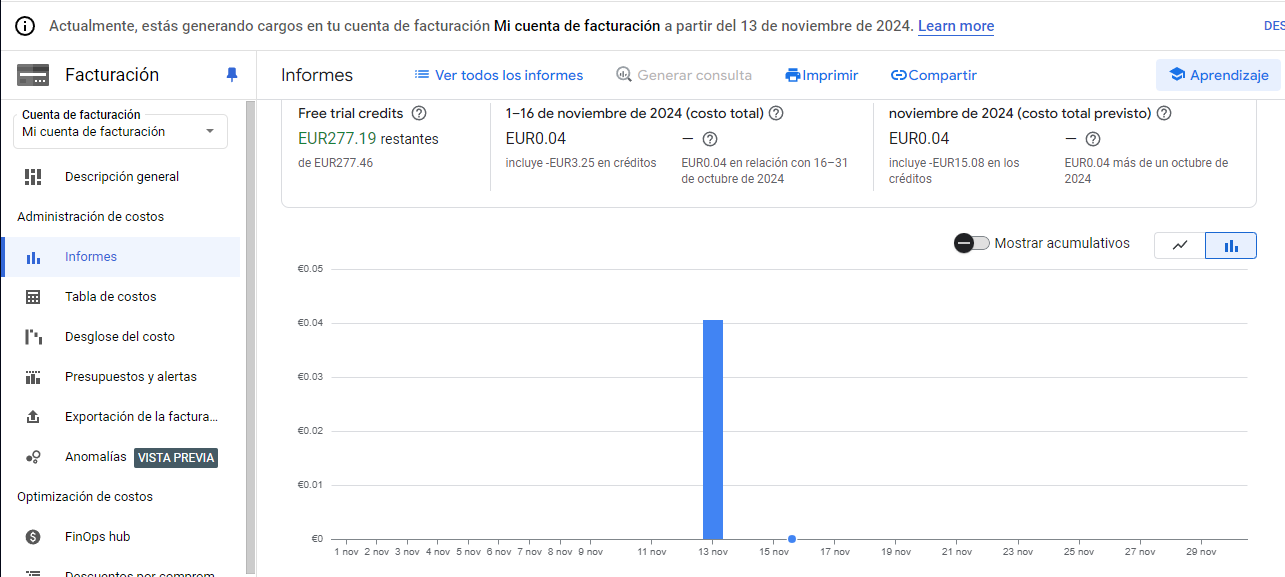
\includegraphics[width=0.8\textwidth]{cloud-console} % Ruta del archivo de la imagen
	\caption{Interfaz de Facturación de Cloud Console.} % Pie de la imagen
	\label{fig:cloud_console} % Etiqueta para referenciar
\end{figure}

Pasado el período de tres meses, la cantidad que supone un umbral de coste se reduce a los 200 euros. En la imagen \ref{fig:cloud_console} se puede ver como se inicia otro proceso de facturación diferente. Supondría por tanto algo a tener en cuenta si se despliega la aplicación en versiones tempranas en el repositorio de aplicaciones de Android puesto que las peticiones no serían solo de una persona, en este caso el desarrollador sino del público en general. La misma consideración habría que hacer si durante el desarrollo se cede el proceso de pruebas a varias personas que puedan hacer la función de beta-testers disparando el consumo de peticiones y por tanto el gasto.
Para el caso de Eco City Tours se supone que el desarrollo y el mayor volumen de peticiones se concentran en los tres primeros meses donde el umbral de gasto es más alto, las pruebas las realiza el propio desarrollador que tendrá acceso al panel de Google Cloud para controlar los posibles gastos y la publicación de la aplicación será en un momento en el que el propio beneficio generado contrarreste los gastos en los que se pueda incurrir.
\subsubsection{Conclusiones}
\textbf{El desarrollo de la aplicación se estima en 4 meses} por el equipo auto gestionado por un solo desarrollador. No se tienen en cuenta alquileres de oficinas o co-working ya que se plantea la posibilidad de teletrabajar, pudiendo trabajar de manera deslocalizada ahorrando así costes. Teniendo en cuenta lo anteriormente citado obtenemos la siguiente tabla resumen:
\tablaSmallSinColores
{Costes totales de \textit{Eco City Tours}} % Título de la tabla
{lc} % Formato de las columnas (l: izquierda, c: centrado)
{costes-totales} % Etiqueta para referencias cruzadas
{%
	\textbf{Concepto} & \textbf{Coste}  \\ % Cabecera
}
{%
	Mano de obra & 8.000€ \\ 
	Hardware & 580€  \\ 
	Internet & 135€ \\ 
	Software & 0€ \\ 
	Servicios Google & 0€ \\ 
	Revisión y auditoría del tutor & 750€ \\ 
	\midrule
	\textbf{Total} & \textbf{9.465 €} \\ 
}

Se ha incluido un coste estimado de 750 € por las tareas de \textbf{revisión y auditoría realizadas por el tutor}. Este coste considera una dedicación de 30 horas, remuneradas a un coste promedio de 25 €/hora, que incluye reuniones, revisiones parciales y finales del proyecto.


Una vez analizado los costes devengados de la creación de la aplicación el beneficio de su explotación debe ser mayor al gasto ocasionado por su creación. Además, una vez publicada la aplicación en la \textit{Play Store} el beneficio obtenido por su explotación debe compensar el tiempo requerido por el personal en horas de mantenimiento de los posibles problemas que pueda experimentar como por ejemplo problemas por actualización de los componentes claves como modelos LLM, que puedan quedar obsoletos. El beneficio de la aplicación puede provenir de varias fuentes en función del modelo de explotación que se eligiese:
\begin{itemize}
	\item \textbf{Ingresos por descarga:} si la aplicación tiene un precio por descarga, los ingresos corresponderían al dinero obtenido menos una comisión del 15\% cobrada por Google por cada venta \cite{googleplay_commission}. Inicialmente, se propone un precio aproximado de lanzamiento de 5 euros, considerando que se obtendrían aproximadamente 4,40 euros como beneficio por descarga. Este precio se estima razonable para incentivar descargas durante la fase inicial. Tras un periodo de prueba, el precio podría ajustarse en función del número de descargas y del comportamiento de los usuarios. Los gastos derivados del uso de servicios externos, como peticiones a APIs, se compensarían con un equilibrio entre usuarios que realicen menos consultas y aquellos más demandantes, garantizando siempre un beneficio estimado en el modelo económico.
	
	\item{Publicidad:} empresas o entidades colaboradoras podrían financiar el desarrollo con publicidad siempre que ésta no suponga una perdida de independencia en los resultados de los modelos, fomente el turismo ecológico y no sea invasiva ni perjudique la experiencia de usuario.
\end{itemize}

\subsection{Viabilidad legal}
Al utilizar los servicios ofrecidos por Google, la compañía se convierte en un socio en el que se delegan muchas de las responsabilidades legales, técnicas y de cumplimiento normativo. Esto simplifica la implementación de Eco City Tours, a la vez que se adquieren ciertos compromisos con el gigante tecnológico. 

\subsubsection{Licencias de uso de las API de Google}
Cada API tiene sus propios términos de uso \cite{google_cloud_terms} y se tiene que tener en cuenta los siguientes aspectos:
\begin{itemize}
	\item \textbf{Uso permitido:} Las API deben ser utilizadas únicamente para finalidades relacionadas con el proyecto.
	\item \textbf{Prohibiciones:} Se prohíbe el \textit{scraping}, almacenamiento de datos más allá de los límites permitidos o redistribución no autorizada.
\end{itemize}

Restricciones específicas:
\begin{itemize}
	\item \textit{Generative AI:} Regulada por políticas relacionadas con el uso de datos generados, especialmente en contextos comerciales.
	\item \textit{Places API y Directions API:} Restringen el almacenamiento y redistribución de los datos obtenidos.
	\item \textit{Maps SDK for Android:} Requiere incluir el logotipo de Google y atribuciones visibles en la interfaz.
\end{itemize}

Los servicios de Google tienen modelos de precios basados en uso para lo que es legalmente\textbf{ obligatorio registrar un método de pago válido} en tu cuenta de Google Cloud para garantizar la continuidad del servicio.

\subsubsection{Privacidad de datos}

El cumplimiento de normativas sobre protección de datos es fundamental:

\begin{itemize}
	\item \textbf{GDPR:} Si se cumplen algunos de los trabajos futuros de la aplicación, ésta recogería datos del usuario, si es un ciudadano europeo debe:
	\begin{itemize}
		\item Firmar un \textit{Acuerdo de Procesamiento de Datos} (DPA) con Google.
		\item La aplicación debe mostrar cómo se manejan los datos obtenidos.
	\end{itemize}
\end{itemize}

Se debe informar a los usuarios que los datos están sujetos a las Políticas de privacidad de Google.

\subsubsection{Restricciones geográficas}

Algunas API tienen restricciones en determinados países debido a leyes locales o sanciones internacionales. 


\subsubsection{Propiedad intelectual}

Los datos obtenidos a través de las API de Google (como mapas y lugares) son propiedad intelectual de Google.


\begin{itemize}
	\item \textbf{Prohibiciones:}
	\begin{itemize}
		\item No se puede almacenar ni redistribuir datos más allá de los límites permitidos.
		\item No se puede usar los datos para minería o análisis masivo sin autorización.
	\end{itemize}
\end{itemize}

\subsubsection{Cumplimiento con normas de publicación}

Para poder publicar la aplicación en el repositorio de aplicaciones Android hay que especificar claramente la política de privacidad y detallar el uso de los servicios.


\subsubsection{Lista a cumplir para viabilidad legal}

\begin{enumerate}
	\item Revisar términos de uso de cada API.
	\item Registrar método de pago.
	\item Cumplir con las normativas de privacidad (GDPR, CCPA).
	\item Incluir atribuciones visibles en la interfaz de usuario.
	\item Respetar las restricciones de almacenamiento y uso de datos.
	\item Desarrollar y publicar una política de privacidad clara para los usuarios.
\end{enumerate}

Respetando el uso ético de la aplicación y cumpliendo con estos requisitos la viabilidad legal de Eco City Tours estaría cumplida y no supondría un impedimento para su ejecución.
\apendice{Especificación de Requisitos}

\section{Introducción}
En esta sección se presentan los requisitos de la aplicación, abordando tanto los objetivos generales como los específicos del proyecto. Se incluye un catálogo detallado de los requisitos funcionales y no funcionales, que definen el comportamiento y las características técnicas de la aplicación. Además, se proporciona una especificación detallada de los requisitos a través de tablas de casos de uso, complementadas con su respectivo diagrama de casos de uso, lo que facilita una comprensión clara de las interacciones principales de los usuarios con el sistema.


\section{Objetivos generales}
La misión fundamental de este proyecto persigue conseguir los siguientes propósitos:
\begin{itemize}
	\item \textbf{Fomentar el turismo sostenible:} Facilitar a los usuarios la exploración de ciudades y zonas rurales promoviendo al mostrar rutas no motorizadas y modos de transporte como caminar y el uso de bicicletas.
	
	\item \textbf{Optimización de experiencias turísticas personalizadas:} Ofrecer a los usuarios rutas personalizadas que se ajusten a sus intereses y preferencias, proporcionando información detallada y relevante sobre los puntos de interés seleccionados.
	
	\item \textbf{Promover el uso de tecnologías inteligentes en el turismo:} Utilizar tecnologías avanzadas como servicios GIS, Google Places y LLM para mejorar la experiencia del usuario, facilitando la generación automática de rutas y la obtención de información actualizada sobre los destinos turísticos.
	
	\item \textbf{Mejorar la accesibilidad a la información turística:} Proporcionar una plataforma fácil de usar que permita a los usuarios acceder rápidamente a descripciones, fotos y otros datos sobre los puntos de interés, mejorando su experiencia de exploración.
	
	\item \textbf{Rutas generadas sin intereses comerciales:} Generar rutas turísticas sin influencias comerciales, ofreciendo una experiencia imparcial y auténtica, en contraste con otras aplicaciones de recomendaciones de viajes.
\end{itemize}

\section{Catálogo de requisitos}
\subsection{Requisitos funcionales}
\begin{itemize}
	\item \textbf{RF-1 Solicitar permisos de uso de GPS:} La aplicación solicitará el permiso para acceder al GPS cuando se inicie por primera vez, ya que es necesario para calcular y mostrar la ubicación del usuario en tiempo real.
	
	\item \textbf{RF-2 Solicitud de activación de GPS:} Si el GPS está desactivado, la aplicación redirigirá a una pantalla que indicará al usuario la necesidad de activarlo para el correcto funcionamiento de la aplicación.
	
	\item \textbf{RF-3 Activación/Desactivación de seguimiento de usuario:} La aplicación mostrará en tiempo real el recorrido del usuario en el mapa, y este seguimiento podrá activarse o desactivarse en cualquier momento mediante un botón.
	
	\item \textbf{RF-4 Centrar la situación actual del usuario sobre el mapa:} El usuario podrá centrar manualmente su posición en el mapa mediante un botón dedicado. Además, existe la opción de fijar la ubicación del usuario en el centro del mapa durante su recorrido.
	
	\item \textbf{RF-5 Configuración de las preferencias del tour:} El usuario rellenará un formulario indicando el lugar que desea visitar, la cantidad de puntos de interés que quiere ver, sus preferencias de transporte (a pie o bicicleta), sus intereses, y el tiempo máximo que quiere dedicar a la ruta.
	
	\item \textbf{RF-6 Cálculo de información a través de un LLM:} La aplicación usará un servicio Gemini para generar los puntos de interés de acuerdo con las propiedades de configuración de la ruta. Además, un servicio Google Places mejorará los datos proporcionando descripciones, fotos, URL, ratings y número de votos de los \acrshort{pdi}.
	
	\item \textbf{RF-7 Eliminación de \acrshort{pdi}:} El usuario podrá eliminar puntos de interés tanto desde la pantalla del mapa como desde el resumen de la ruta. Cada vez que un \acrshort{pdi} es eliminado o añadido, la ruta se recalcula automáticamente para ofrecer el trayecto más óptimo.
	
	\item \textbf{RF-8 Cálculo de ruta optimizada:} La aplicación calculará la ruta más corta que conecte los puntos de interés seleccionados por el usuario, adaptándose al medio de transporte elegido (a pie o bicicleta).
	
	\item \textbf{RF-9 Capacidad de añadir un \acrshort{pdi}:} El usuario podrá agregar manualmente un lugar introduciendo su nombre en la barra de búsqueda. Si el lugar existe en los servicios de Google, será añadido automáticamente a la ruta; de lo contrario, no se tomará ninguna acción.
	
	\item \textbf{RF-10 Unirse a Eco City Tour:} El usuario podrá unirse a la ruta existente en cualquier momento. La aplicación calculará la ruta más corta para conectarlo con el tour.
	
	\item \textbf{RF-11 Mejora de los puntos de interés con servicio de obtención de información:} Los datos de los puntos de interés se enriquecerán con información adicional obtenida de Google Places, incluyendo ratings, imágenes, URL y número de votos, mejorando la experiencia del usuario.
	
	\item \textbf{RF-12 Guardado y carga de las rutas turísticas:} el usuario podrá guardar los tours que quiera y tendrá acceso a los mismos desde la pantalla de configuración del Eco City Tour.
	
\end{itemize}

\subsection{Requisitos no funcionales}
\begin{itemize}
	\item \textbf{RNF-1 Rendimiento:} la aplicación debe demostrar un tiempo de respuesta aceptable para que su manejo sea fluido y la carga de datos sea razonable al enlazar varios servicios asíncronos, de tal manera que no se perjudique la experiencia de usuario. 
	\item \textbf{RNF-2 Usabilidad:} Eco City Tours debe ser intuitiva y fácil de entender y utilizar.
	\item \textbf{RNF-3 Disponibilidad:} la aplicación debe estar disponible independientemente de la localización del usuario.
	\item \textbf{RNF-4 Mantenibilidad:} la aplicación debe ser fácilmente modificable debido a su carácter modular, facilitando el mantenimiento para el desarrollador. Además, \textbf{el uso de SonarCloud} ayuda a asegurar la calidad del código mediante el análisis continuo, lo que permite identificar y corregir errores potenciales y optimizar el código, favoreciendo así la mantenibilidad a largo plazo.
	
	\item \textbf{RNF-5 Escalabilidad:} Eco City Tours debe ser capaz de gestionar eficientemente un crecimiento continuo en el número de usuarios, adaptándose sin problemas para ofrecer un rendimiento óptimo incluso en situaciones de alta demanda.
	\item \textbf{RNF-6 Soporte:} la aplicación debe funcionar en versiones actuales de Android sin problemas de rendimiento o fallos en alguna de sus funcionalidades.
\end{itemize}
\clearpage

\section{Especificación de requisitos}

\subsection{Actores del sistema}

\begin{table}[H]
	\centering
	\begin{tabularx}{\linewidth}{ p{0.21\columnwidth} p{0.71\columnwidth} }
		\toprule
		\textbf{Actor}    & A01 \\
		\toprule
		\textbf{Nombre:} 			  & \textbf{Usuario} \\
		\textbf{Versión}              & 1.0    \\
		\textbf{Autor}                & \autor \\
		\textbf{Descripción}          & Persona que interactúa con la aplicación Eco City Tour para generar y gestionar rutas turísticas personalizadas. \\
		\textbf{Tipo}                 & Usuario \\
		\textbf{Objetivo}             & Generar, visualizar y personalizar rutas turísticas basadas en puntos de interés y preferencias personales. \\
		\textbf{Responsabilidades}    & 
		\begin{itemize}
			\tightlist
			\item Completar el formulario de preferencias para generar una ruta.
			\item Visualizar detalles de puntos de interés.
			\item Añadir o eliminar puntos de interés de la ruta.
			\item Iniciar y detener el seguimiento de ubicación.
		\end{itemize}\\
		\textbf{Relaciones con casos de uso} & CU01(\ref{cu:config-parametros}), CU02.1(\ref{cu:visualizar-detalles}), CU2.2(\ref{cu:eliminar-pdi}), CU04(\ref{cu:guardar-tour}), CU05(\ref{cu:cargar-tour}). \\
		\bottomrule
	\end{tabularx}
	\caption{A01 - Usuario}
	\label{actor:usuario}
\end{table}

\begin{table}[H]
	\centering
	\begin{tabularx}{\linewidth}{ p{0.21\columnwidth} p{0.71\columnwidth} }
		\toprule
		\textbf{Actor}    & A02 \\
		\toprule
		\textbf{Nombre:} 			  & \textbf{Cloud Firestore} \\
		\textbf{Versión}              & 1.0    \\
		\textbf{Autor}                & \autor \\
		\textbf{Descripción}          & Servicio que posibilita el guardado y carga de las rutas obtenidas por la aplicación. \\
		\textbf{Tipo}                 & Sistema \\
		\textbf{Objetivo}             & Guardar y cargar Eco City Tours generados por el Usuario~(\ref{actor:usuario}). \\
		\textbf{Responsabilidades}    & 
		\begin{itemize}
			\tightlist
			\item Guardar ruta generada.
			\item Cargar en el mapa el Eco City Tour guardado en base de datos.
			\item Borrar los Eco City Tour almacenados.
		\end{itemize}\\
		\textbf{Relaciones con casos de uso} & CU04(\ref{cu:guardar-tour}), CU05(\ref{cu:cargar-tour}) \\
		\bottomrule
	\end{tabularx}
	\caption{A02 - Cloud Firestore}
	\label{actor:firestore}
\end{table}


\begin{table}[H]
	\centering

	\begin{tabularx}{\linewidth}{ p{0.21\columnwidth} p{0.71\columnwidth} }
		\toprule
		\textbf{Actor-ID}    & A03 \\
		\toprule
		\textbf{Nombre: } 			  & \textbf{Gemini-pro 1.5} \\
		\textbf{Versión}              & 1.0    \\
		\textbf{Autor}                & \autor \\
		\textbf{Descripción}          & Servicio externo que proporciona una lista de puntos de interés (POI) basados en las propiedades de configuración de la ruta. \\
		\textbf{Tipo}                 & Sistema \\
		\textbf{Objetivo}             & Suministrar información relevante sobre puntos de interés en función de los criterios del usuario. \\
		\textbf{Responsabilidades}    & 
		\begin{itemize}
			\tightlist
			\item Consultar la información de \acrshort{pdi} según las preferencias de búsqueda del usuario.
			\item Enviar los datos de los \acrfull{pdi} a la aplicación para generar la ruta.
		\end{itemize}\\
		\textbf{Relaciones con casos de uso} & CU01.1(\ref{cu:calcular-tour})\\
		\bottomrule
	\end{tabularx}
	\caption{A03 - Gemini Pro 1.5}
	\label{actor:gemini}
\end{table}

\begin{table}[H]
	\centering

	\begin{tabularx}{\linewidth}{ p{0.21\columnwidth} p{0.71\columnwidth} }
		\toprule
		\textbf{Actor-ID}    & A04 \\
		\toprule
		\textbf{Nombre: } 			  & \textbf{Google Places Service} \\
		\textbf{Versión}              & 1.0    \\
		\textbf{Autor}                & \autor \\
		\textbf{Descripción}          & Servicio externo encargado de mejorar la información sobre los puntos de interés proporcionando detalles adicionales como descripciones, fotos y valoraciones. \\
		\textbf{Tipo}                 & Sistema \\
		\textbf{Objetivo}             & Enriquecer la información de los \acrlong{pdi} para que el usuario obtenga datos detallados y actualizados sobre cada lugar. \\
		\textbf{Responsabilidades}    & 
		\begin{itemize}
			\tightlist
			\item Proveer información detallada sobre los \acrshort{pdi}.
			\item Enviar las descripciones, fotos y valoraciones de los \acrshort{pdi} a la aplicación.
		\end{itemize}\\
		\textbf{Relaciones con casos de uso} & CU01.1 (\ref{cu:calcular-tour})\\
		\bottomrule
	\end{tabularx}
	\caption{A04 - Google Places Service}
	\label{actor:google-places}
\end{table}

\begin{table}[H]
	\centering

	\begin{tabularx}{\linewidth}{ p{0.21\columnwidth} p{0.71\columnwidth} }
		\toprule
		\textbf{Actor-ID}    & A05 \\
		\toprule
		\textbf{Nombre: } 			  & \textbf{Google Direction Service} \\
		\textbf{Versión}              & 1.0    \\
		\textbf{Autor}                & \autor \\
		\textbf{Descripción}          & Servicio externo encargado de generar una ruta actualizada entre los \acrshort{pdi} que componen el Eco City Tour. \\
		\textbf{Tipo}                 & Sistema \\
		\textbf{Objetivo}             & Proveer la mejor ruta a mostrar en el mapa que conecte los \acrshort{pdi} de cada \textit{Eco City Tour} en cada momento. \\
		\textbf{Responsabilidades}    & 
		\begin{itemize}
			\tightlist
			\item Generar el camino que ha de seguir el usuario de manera más corta según el medio de transporte elegido.
			\item Actualizar en cada momento el camino más corto entre los distintos lugares.
		\end{itemize}\\
		\textbf{Relaciones con casos de uso} & CU01.1 (\ref{cu:calcular-tour})CU02 (\ref{cu:navegar-mapa}) \\
		\bottomrule
	\end{tabularx}
	\caption{A05 - Google Direction Service}
	\label{actor:google-directions}
\end{table}

\begin{table}[H]
	\centering
	\begin{tabularx}{\linewidth}{ p{0.21\columnwidth} p{0.71\columnwidth} }
		\toprule
		\textbf{Actor-ID}    & A06 \\
		\toprule
		\textbf{Nombre: }			  & \textbf{Crashlytics} \\
		\textbf{Versión}              & 1.0    \\
		\textbf{Autor}                & \autor \\
		\textbf{Descripción}          & Servicio externo encargado de registrar en todo momento si se produce un error en la ejecución de la aplicación. \\
		\textbf{Tipo}                 & Sistema \\
		\textbf{Objetivo}             & Dejar constancia en un log de los errores que se puedan llevar a cabo en la ejecución. \\
		\textbf{Responsabilidades}    & 
		\begin{itemize}
			\tightlist
			\item Detectar errores fatales en la ejecución de la aplicación.
			\item Registrar en la nube los detalles que formaron la excepción, para posterior análisis.
		\end{itemize}\\
		\textbf{Relaciones con casos de uso} & CU06 (\ref{cu:registro-log}) \\
		\bottomrule
	\end{tabularx}
	\caption{A06 - Crashlytics}
		\label{actor:crashlytics}
\end{table}

\subsection{Casos de uso}
\label{subsec:casos-uso}

\subsection{CU00 - Caso de uso de inicialización. Configuración GPS}
\begin{figure}[H]
	\centering
	\includegraphics[scale=0.6]{CU00-Gestión-de-GPS}
	\caption{Diagrama de caso de uso CU00 - Configuración GPS}
	\label{fig:CU00-Gestión-de-GPS}
\end{figure}

Este caso de uso es fundamental, ya que sin el permiso de GPS o la activación del sensor, el resto de funcionalidades de la aplicación no pueden ejecutarse. Para mayor claridad y facilitar la lectura de los diagramas restantes, se presenta por separado, destacando su papel como requisito previo para las demás operaciones.

\begin{table}[H]
	\centering
	\begin{tabularx}{\linewidth}{ p{0.21\columnwidth} p{0.71\columnwidth} }
		\toprule
		\textbf{CU00}    & \textbf{Configuración GPS} \\
		\toprule
		\textbf{Versión}              & 1.0    \\
		\textbf{Actor}                & A01 Usuario (\ref{actor:usuario}) \\
		\textbf{Autor}                & \autor \\
		\textbf{Requisitos asociados} & RF-1, RF-2 \\
		\textbf{Descripción}          & Configura la aplicación para tener acceso a la ubicación mediante GPS. \\
		\textbf{Precondición}         & La aplicación está instalada y abierta por primera vez o tras haber revocado permisos anteriormente. \\
		\textbf{Acciones}             &
		\begin{enumerate}
			\def\labelenumi{\arabic{enumi}.}
			\tightlist
			\item La aplicación solicita permiso para el uso del GPS.
			\item El usuario concede el permiso.
			\item La aplicación detecta si el GPS está activado.
			\item Si el GPS no está activado, solicita al usuario activarlo.
		\end{enumerate}\\
		\textbf{Postcondición}        & La aplicación tiene acceso a la ubicación en tiempo real. \\
		\textbf{Excepciones}          & 
		\begin{itemize}
			\tightlist
			\item El usuario no concede el permiso de GPS.
			\item El usuario no activa el GPS cuando se le solicita.
		\end{itemize}\\
		\textbf{Importancia}          & Alta \\
		\textbf{Casos de Prueba}      & 
		\begin{itemize}
			\tightlist
			\item \textbf{Prueba 1 - Permiso concedido:} La aplicación solicita y obtiene acceso al GPS cuando el usuario concede el permiso.\vspace{2pt}
			\item \textbf{Prueba 2 - Permiso denegado:} El usuario deniega el permiso. La aplicación no avanza al mapa y no permite operar sobre la aplicación. \vspace{2pt}
			\item \textbf{Prueba 3 - GPS desactivado:} El GPS está apagado. La aplicación solicita activación y detecta si el usuario lo enciende.
		\end{itemize}\\
		\bottomrule
	\end{tabularx}
	\caption{CU00 Configuración GPS}
\end{table}



\subsection{Casos de uso general}

\begin{figure}[H]
	\centering
	\hspace*{-2cm}
	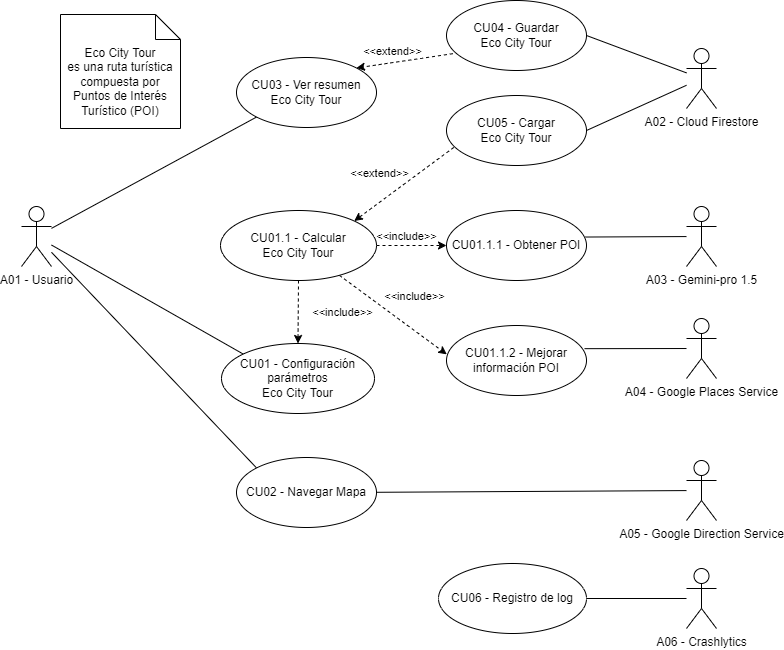
\includegraphics[scale=0.6]{casos-de-uso}
	\caption{Diagrama de casos de uso general de Eco City Tours}
	\label{fig:casos-de-uso}
\end{figure}

\subsection{CU01 - Configuración de parámetros Eco City Tour}

\begin{table}[H]
	\centering
	\begin{tabularx}{\linewidth}{ p{0.21\columnwidth} p{0.71\columnwidth} }
		\toprule
		\textbf{CU01}    & \textbf{Configuración parámetros Eco City Tour} \\
		\toprule
		\textbf{Versión}              & 1.0    \\
		\textbf{Actor}                & A01 Usuario (\ref{actor:usuario}) \\
		\textbf{Autor}                & \autor \\
		\textbf{Requisitos asociados} & RF-5 \\
		\textbf{Descripción}          & Configurar los parámetros necesarios para generar un Eco City Tour personalizado según las propiedades de configuración de la ruta. \\
		\textbf{Precondición}         & El usuario accede a la pantalla de configuración. \\
		\textbf{Acciones}             &
		\begin{enumerate}
			\def\labelenumi{\arabic{enumi}.}
			\tightlist
			\item El usuario completa el formulario de preferencias, incluyendo el lugar, número de \acrshort{pdi}, selecciona un asistente \acrshort{ia} (cultura, aventura o romántico), selecciona un medio de transporte y tiempo máximo.
		\end{enumerate}\\
		\textbf{Postcondición}        & Los parámetros quedan configurados y listos para generar la ruta. \\
		\textbf{Excepciones}          & 
		\begin{itemize}
			\tightlist
			\item El usuario no completa el formulario de configuración.
			\item Error en la carga de los datos de configuración.
		\end{itemize}\\
		\textbf{Importancia}          & Alta \\
		\textbf{Casos de Prueba}      &
		\begin{itemize}
			\item \textbf{Prueba 1 - Configuración correcta:} El usuario completa el formulario correctamente con todos los campos requeridos. El sistema guarda los parámetros y los muestra confirmados en el log del modo debug.
			\vspace{2pt}
			\item \textbf{Prueba 2 - Campos vacíos:} El usuario deja el formulario sin modificar. El sistema muestra un \textit{Eco City Tour} en la mejor ciudad del mundo: Salamanca.
			\vspace{2pt}
			\item \textbf{Prueba 3 - Valores límites:} El usuario introduce valores límite en los campos. El sistema valida los parámetros y los procesa correctamente.
		\end{itemize} \\
		\bottomrule
	\end{tabularx}
	\caption{CU01 Configuración parámetros Eco City Tour}
	\label{cu:config-parametros}
\end{table}


\subsection{CU01.1 - Calcular \gls{eco-city-tour}[]}

\begin{table}[H]
	\centering
	\begin{tabularx}{\linewidth}{ p{0.21\columnwidth} p{0.71\columnwidth} }
		\toprule
		\textbf{CU01.1}    & \textbf{Calcular Eco City Tour} \\
		\toprule
		\textbf{Versión}              & 1.0    \\
		\textbf{Actor}                & A03 (\ref{actor:gemini}), A04 (\ref{actor:google-places}), A05 (\ref{actor:google-directions}) \\
		\textbf{Autor}                & \autor \\
		\textbf{Requisitos asociados} & RF-6, RF-8 \\
		\textbf{Descripción}          & Generar una ruta optimizada conectando los puntos de interés seleccionados en función de las propiedades de configuración de la ruta. \\
		\textbf{Precondición}         & Los parámetros han sido configurados correctamente. \\
		\textbf{Acciones}             &
		\begin{enumerate}
			\def\labelenumi{\arabic{enumi}.}
			\tightlist
			\item El usuario confirma la configuración de preferencias.
			\item El sistema consulta un LLM para obtener \acrshort{pdi} basados en las propiedades de configuración de la ruta.
			\item El sistema envía los \acrshort{pdi} a Google Places para obtener información mejorada.
			\item El sistema consulta un servicio de optimización de rutas para generar la ruta optimizada.
		\end{enumerate}\\
		\textbf{Postcondición}        & La ruta optimizada es calculada y lista para ser visualizada. \\
		\textbf{Excepciones}          & 
		\begin{itemize}
			\tightlist
			\item Fallo en la conexión con el LLM.
			\item Error en el servicio de optimización de rutas.
		\end{itemize}\\
		\textbf{Importancia}          & Alta \\
		\textbf{Casos de Prueba}      &
		\begin{itemize}
			\item \textbf{Prueba 1 - Configuración correcta:} El usuario confirma los parámetros correctamente. El sistema calcula la ruta sin errores y muestra los \acrlong{pdi} optimizados.
			\vspace{2pt}
			\item \textbf{Prueba 2 - Fallo en el LLM:} El sistema no obtiene respuesta del LLM. Se muestra un mensaje de error y se sugiere reintentar la consulta.
			\vspace{2pt}
			\item \textbf{Prueba 3 - Servicio de rutas inalcanzable:} El sistema no puede conectarse al servicio de optimización de rutas (Google Directions). El sistema notifica el fallo al usuario y permite volver a intentarlo.
			\vspace{2pt}
			\item \textbf{Prueba 4 - Valores límite en parámetros:} El usuario configura un número mínimo y máximo de \acrshort{pdi}. El sistema muestra correctamente estos valores calculando la ruta.
		\end{itemize} \\
		\bottomrule
	\end{tabularx}
	\caption{CU01.1 Calcular Eco City Tour}
	\label{cu:calcular-tour}
\end{table}


\subsection{CU02 - Navegar en el mapa}


\begin{table}[H]
	\centering
	\begin{tabularx}{\linewidth}{ p{0.21\columnwidth} p{0.71\columnwidth} }
		\toprule
		\textbf{CU02}    & \textbf{Navegar en el mapa} \\
		\toprule
		\textbf{Versión}              & 1.0    \\
		\textbf{Autor}                & \autor \\
		\textbf{Actor}                & A01 Usuario (\ref{actor:usuario}) \\
		\textbf{Requisitos asociados} & RF-4 \\
		\textbf{Descripción}          & El usuario puede desplazarse y explorar el mapa interactivo de la aplicación. \\
		\textbf{Precondición}         & El mapa está visible. \\
		\textbf{Acciones}             &
		\begin{enumerate}
			\def\labelenumi{\arabic{enumi}.}
			\tightlist
			\item El usuario explora el mapa desplazándose y haciendo zoom.
		\end{enumerate}\\
		\textbf{Postcondición}        & El usuario navega por el mapa para observar los \acrshort{pdi} y la ruta. \\
		\textbf{Importancia}          & Media \\
		\textbf{Casos de Prueba}      &
		\begin{itemize}
			\item \textbf{Prueba 1 - Desplazamiento funcional:} El usuario desplaza el mapa arrastrando la pantalla con un gesto táctil. El sistema responde correctamente mostrando las áreas correspondientes sin retraso injustificado.
			\vspace{2pt}
			\item \textbf{Prueba 2 - Zoom funcional:} El usuario realiza gestos de zoom in y zoom out en el mapa. El sistema aumenta y reduce el nivel de zoom de manera fluida.
			\vspace{2pt}
			\item \textbf{Prueba 3 - Carga de marcadores (\acrshort{pdi}):} Al navegar, los puntos de interés (\acrshort{pdi}) se cargan dinámicamente y son visibles sin retrasos en la interfaz.
			\vspace{2pt}
			\item \textbf{Prueba 4 - Valores límites de zoom:} El sistema limita correctamente el nivel de zoom máximo y mínimo, evitando desplazamientos inválidos.
		\end{itemize} \\
		\bottomrule
	\end{tabularx}
	\caption{CU02 Navegar en el mapa}
	\label{cu:navegar-mapa}
\end{table}



\begin{figure}[H]
	\centering
	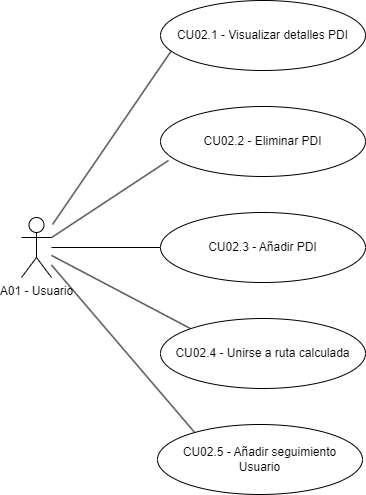
\includegraphics[scale=0.6]{CU02-Navegar-mapa}
	\caption{Diagrama de caso de uso CU02 - Navegar en el mapa}
	\label{CU02-Navegar-mapa}
\end{figure}



\begin{table}[H]
	\centering
	\begin{tabularx}{\linewidth}{ p{0.21\columnwidth} p{0.71\columnwidth} }
		\toprule
		\textbf{CU02.1}    & \textbf{Visualizar detalles de \acrfull{pdi}} \\
		\toprule
		\textbf{Versión}              & 1.0    \\
		\textbf{Actor}                & A01 Usuario (\ref{actor:usuario}) \\
		\textbf{Autor}                & \autor \\
		\textbf{Requisitos asociados} & RF-6, RF-11 \\
		\textbf{Descripción}          & El usuario puede obtener información detallada sobre un punto de interés seleccionado en el mapa. \\
		\textbf{Precondición}         & La ruta y los puntos de interés están visibles en el mapa. \\
		\textbf{Acciones}             &
		\begin{enumerate}
			\def\labelenumi{\arabic{enumi}.}
			\tightlist
			\item El usuario selecciona un marcador de punto de interés en el mapa.
			\item El sistema muestra la información detallada del punto de interés.
		\end{enumerate}\\
		\textbf{Postcondición}        & La información detallada del punto de interés es visible para el usuario. \\
		\textbf{Excepciones}          & 
		\begin{itemize}
			\tightlist
			\item Fallo en la carga de información del \acrlong{pdi} debido a problemas de conectividad.
			\item Error en el servicio externo de obtención de información.
		\end{itemize}\\
		\textbf{Importancia}          & Alta \\
		\textbf{Casos de Prueba}      &
		\begin{itemize}
			\item \textbf{Prueba 1 - Información accesible:} El usuario selecciona un marcador de \acrshort{pdi} en el mapa. El sistema carga y muestra correctamente el nombre, descripción, imagen y detalles del \acrlong{pdi}.
			\vspace{2pt}
			\item \textbf{Prueba 2 - Punto sin detalles:} El marcador seleccionado corresponde a un \acrshort{pdi} que no tiene información asociada. El sistema muestra la imagen por defecto y el texto en blanco.
		\end{itemize} \\
		\bottomrule
	\end{tabularx}
	\caption{CU02.1 Visualizar detalles de los \acrfull{pdi}}
	\label{cu:visualizar-detalles}
\end{table}


\begin{table}[H]
	\centering
	\begin{tabularx}{\linewidth}{ p{0.21\columnwidth} p{0.71\columnwidth} }
		\toprule
		\textbf{CU02.2}    & \textbf{Eliminar \acrlong{pdi}} \\
		\toprule
		\textbf{Versión}              & 1.0    \\
		\textbf{Actor}                & A01 (\ref{actor:usuario}), A05 (\ref{actor:google-directions}) \\
		\textbf{Autor}                & \autor \\
		\textbf{Requisitos asociados} & RF-7, RF-8 \\
		\textbf{Descripción}          & El usuario puede eliminar puntos de interés de la ruta desde el mapa. \\
		\textbf{Precondición}         & La ruta ha sido generada y los puntos de interés están visibles en el mapa. \\
		\textbf{Acciones}             &
		\begin{enumerate}
			\def\labelenumi{\arabic{enumi}.}
			\tightlist
			\item El usuario selecciona un punto de interés en el mapa.
			\item El sistema elimina el punto de interés de la ruta.
			\item El sistema recalcula la ruta optimizada sin el punto eliminado.
		\end{enumerate}\\
		\textbf{Postcondición}        & La ruta es recalculada sin el punto de interés eliminado. \\
		\textbf{Excepciones}          & 
		\begin{itemize}
			\tightlist
			\item Error en el recálculo de la ruta.
			\item Problemas de conectividad al intentar actualizar la ruta.
		\end{itemize}\\
		\textbf{Importancia}          & Media \\
		\textbf{Casos de Prueba}      &
		\begin{itemize}
			\item \textbf{Prueba 1 - Eliminación exitosa:} El usuario selecciona un \acrshort{pdi} y el sistema lo elimina correctamente de la ruta. El recálculo de la ruta es exitoso.
			\vspace{2pt}
			\item \textbf{Prueba 2 - Error en el recálculo:} El sistema no logra recalcular la ruta después de la eliminación del \acrshort{pdi}. Se muestra un mensaje de error y la ruta previa se mantiene visible.
			\vspace{2pt}
		\end{itemize} \\
		\bottomrule
	\end{tabularx}
	\caption{CU02.2 Eliminar \acrlong{pdi}}
	\label{cu:eliminar-pdi}
\end{table}


\begin{table}[H]
	\centering
	\begin{tabularx}{\linewidth}{ p{0.21\columnwidth} p{0.71\columnwidth} }
		\toprule
		\textbf{CU02.3}    & \textbf{Añadir \acrfull{pdi}} \\
		\toprule
		\textbf{Versión}              & 1.0    \\
		\textbf{Actor}                & A01 Usuario \ref{actor:usuario} \\
		\textbf{Autor}                & \autor \\
		\textbf{Requisitos asociados} & RF-8, RF-9 \\
		\textbf{Descripción}          & El usuario puede añadir manualmente un nuevo \acrshort{pdi} a la ruta introduciendo su nombre en la barra de búsqueda. \\
		\textbf{Precondición}         & La ruta ha sido generada previamente. \\
		\textbf{Acciones}             &
		\begin{enumerate}
			\def\labelenumi{\arabic{enumi}.}
			\tightlist
			\item El usuario introduce el nombre de un lugar en la barra de búsqueda.
			\item El sistema muestra el resultado de la búsqueda y el usuario lo selecciona para añadirlo.
			\item El sistema recalcula la ruta optimizada incluyendo el nuevo \acrlong{pdi}.
		\end{enumerate}\\
		\textbf{Postcondición}        & El nuevo lugar es añadido a la ruta, y la ruta optimizada es recalculada. \\
		\textbf{Excepciones}          & 
		\begin{itemize}
			\tightlist
			\item El lugar no se encuentra en el servicio de búsqueda.
			\item Fallo en el recalculo de la ruta.
		\end{itemize}\\
		\textbf{Importancia}          & Baja \\
		\textbf{Casos de Prueba}      &
		\begin{itemize}
			\item \textbf{Prueba 1 - Añadir \acrshort{pdi} exitoso:} El usuario introduce el nombre del lugar, el sistema lo encuentra y lo añade correctamente. La ruta es recalculada y optimizada.
			\vspace{2pt}
			\item \textbf{Prueba 2 - Lugar no encontrado:} El usuario introduce un nombre de lugar inexistente. El sistema muestra el listado de lugares vacío pero permite al usuario volver a buscar otro lugar o volver al mapa.
			\vspace{2pt}
			\item \textbf{Prueba 3 - Cálculo de ruta muy larga:} El usuario selecciona un lugar válido, pero no es el que se esperaba al encontrarse muy lejos. El sistema es capaz de ejecutar el cálculo aunque le lleve más tiempo al ser una tarea síncrona. El \acrshort{pdi} se puede eliminar manualmente por el usuario.
		\end{itemize} \\
		\bottomrule
	\end{tabularx}
	\caption{CU02.3 Añadir \acrfull{pdi}}
	\label{cu:añadir-pdi}
\end{table}


\begin{table}[H]
	\centering
	\begin{tabularx}{\linewidth}{ p{0.21\columnwidth} p{0.71\columnwidth} }
		\toprule
		\textbf{CU02.4}    & \textbf{Unirse a la ruta calculada} \\
		\toprule
		\textbf{Versión}              & 1.0    \\
		\textbf{Actor}                & A01 Usuario \ref{actor:usuario} \\
		\textbf{Autor}                & \autor \\
		\textbf{Requisitos asociados} & RF-10 \\
		\textbf{Descripción}          & Permite al usuario unirse a una ruta previamente generada desde su ubicación actual. \\
		\textbf{Precondición}         & Una ruta ya ha sido generada y está activa. No hace falta que esté activado el seguimiento en vivo. \\
		\textbf{Acciones}             &
		\begin{enumerate}
			\def\labelenumi{\arabic{enumi}.}
			\tightlist
			\item El usuario selecciona la opción para unirse a la ruta desde su ubicación actual.
			\item El sistema calcula la ruta más corta para conectar la ubicación actual del usuario con la ruta generada.
		\end{enumerate}\\
		\textbf{Postcondición}        & El usuario es guiado desde su ubicación actual hasta la ruta generada. \\
		\textbf{Excepciones}          & 
		\begin{itemize}
			\tightlist
			\item Error en el cálculo de la ruta de conexión.
		\end{itemize}\\
		\textbf{Importancia}          & Media \\
		\textbf{Casos de Prueba}      &
		\begin{itemize}
			\item \textbf{Prueba 1 - Unirse a la ruta exitosa:} El usuario selecciona la opción para unirse y el sistema calcula correctamente la ruta de conexión.
			\vspace{2pt}
			\item \textbf{Prueba 2 - Ubicación inválida:} El sistema no puede determinar la ubicación actual del usuario. Se muestra la unión al punto más cercano viable del usuario. p.e. si está en mitad del mar lo situaría en la costa.
			\vspace{2pt}
			\item \textbf{Prueba 3 - Ruta previa no generada:} El usuario intenta unirse sin que exista una ruta activa pues es el único punto de la ruta. No se muestra ninguna ruta pero la ubicación formará parte de ella si se añade otra ruta.
			\vspace{2pt}
			\item \textbf{Prueba 4 - Unirse a ruta si está ya unido:} El usuario no puede tener activado el botón de unirse a ruta para evitar el conflicto de unirse múltiples veces.
		\end{itemize} \\
		\bottomrule
	\end{tabularx}
	\caption{CU02.4 Unirse a la ruta calculada}
	\label{cu:unirse-ruta}
\end{table}


\begin{table}[H]
	\centering
	\begin{tabularx}{\linewidth}{ p{0.21\columnwidth} p{0.71\columnwidth} }
		\toprule
		\textbf{CU02.5}    & \textbf{Añadir seguimiento del usuario} \\
		\toprule
		\textbf{Versión}              & 1.0    \\
		\textbf{Actor}                & A01 Usuario (\ref{actor:usuario}) \\
		\textbf{Autor}                & \autor \\
		\textbf{Requisitos asociados} & RF-3 \\
		\textbf{Descripción}          & Permite al usuario activar o desactivar el seguimiento de su posición en tiempo real en el mapa. \\
		\textbf{Precondición}         & La aplicación tiene acceso a la ubicación del usuario. \\
		\textbf{Acciones}             &
		\begin{enumerate}
			\def\labelenumi{\arabic{enumi}.}
			\tightlist
			\item El usuario selecciona la opción de activar o desactivar el seguimiento de su ubicación en el mapa.
			\item El sistema ajusta el mapa para mostrar o dejar de mostrar el movimiento del usuario en tiempo real.
		\end{enumerate}\\
		\textbf{Postcondición}        & El mapa sigue o deja de seguir la posición del usuario en tiempo real. \\
		\textbf{Excepciones}          & 
		\begin{itemize}
			\tightlist
			\item Problemas de conexión con el GPS.
			\item Pérdida de señal GPS.
		\end{itemize}\\
		\textbf{Importancia}          & Baja \\
		\textbf{Casos de Prueba}      &
		\begin{itemize}
			\item \textbf{Prueba 1 - Seguimiento activado:} El usuario activa el seguimiento. El mapa ajusta su vista en tiempo real conforme a la ubicación del usuario.
			\vspace{2pt}
			\item \textbf{Prueba 2 - Seguimiento desactivado:} El usuario desactiva el seguimiento. El mapa deja de ajustarse a la posición del usuario.
			\vspace{2pt}
			\item \textbf{Prueba 3 - Señal GPS débil:} La señal del GPS se pierde temporalmente. El sistema mantendrá la ubicación del usuario en la última ubicación proporcionada (realizado por el Sistema).
		\end{itemize} \\
		\bottomrule
	\end{tabularx}
	\caption{CU02.5 Añadir seguimiento del usuario}
	\label{cu:añadir-seguimiento}
\end{table}



\subsection{CU03 - Ver resumen Eco City Tour}
\begin{table}[H]
	\centering
	\begin{tabularx}{\linewidth}{ p{0.21\columnwidth} p{0.71\columnwidth} }
		\toprule
		\textbf{CU03}    & \textbf{Ver resumen Eco City Tour} \\
		\toprule
		\textbf{Versión}              & 1.0    \\
		\textbf{Actor}                & A01 Usuario \ref{actor:usuario} \\
		\textbf{Autor}                & \autor \\
		\textbf{Requisitos asociados} & RF-4, RF-8 \\
		\textbf{Descripción}          & Muestra un resumen de la ruta generada, incluyendo la distancia, duración y medio de transporte. \\
		\textbf{Precondición}         & La ruta ha sido generada. \\
		\textbf{Acciones}             &
		\begin{enumerate}
			\def\labelenumi{\arabic{enumi}.}
			\tightlist
			\item El usuario accede a la pantalla de resumen.
			\item La aplicación muestra los detalles de la ruta, incluyendo distancia total, tiempo estimado y transporte elegido.
		\end{enumerate}\\
		\textbf{Postcondición}        & El resumen es visible para el usuario. \\
		\textbf{Excepciones}          & 
		\begin{itemize}
			\tightlist
			\item Error en la carga de los datos de la ruta.
		\end{itemize}\\
		\textbf{Importancia}          & Baja \\
		\textbf{Casos de Prueba}      &
		\begin{itemize}
			\item \textbf{Prueba 1 - Resumen completo visible:} El usuario accede a la pantalla de resumen y todos los detalles (distancia, duración y transporte) se muestran correctamente.
			\vspace{2pt}
			\item \textbf{Prueba 2 - Valores límite de distancia y tiempo:} Validar que el sistema maneja correctamente valores grandes (e.g., rutas muy largas) y pequeños (e.g., rutas cortas de menos de 1 km).
			\vspace{2pt}
			\item \textbf{Prueba 3 - Eco City Tour vacío:} Desde la pantalla se eliminan todos los \acrshort{pdi} lo que devuelve al usuario a la pantalla del mapa pues no tiene información útil que mostrar.
		\end{itemize} \\
		\bottomrule
	\end{tabularx}
	\caption{CU03 Ver resumen Eco City Tour}
	\label{cu:resumen}
\end{table}


\subsection{CU04 - Guardar Eco City Tour}
\begin{table}[H]
	\centering
	
	\begin{tabularx}{\linewidth}{ p{0.21\columnwidth} p{0.71\columnwidth} }
		\toprule
		\textbf{CU04}    & \textbf{Guardar Eco City Tour} \\
		\toprule
		\textbf{Versión}              & 1.0    \\
		\textbf{Actor}                & A01~\ref{actor:usuario}, A02~\ref{actor:firestore} \\
		\textbf{Autor}                & \autor \\
		\textbf{Requisitos asociados} & RF-12 \\
		\textbf{Descripción}          & Permite al usuario guardar la ruta generada para acceder a ella en el futuro. \\
		\textbf{Precondición}         & La ruta ha sido generada. \\
		\textbf{Acciones}             &
		\begin{enumerate}
			\def\labelenumi{\arabic{enumi}.}
			\tightlist
			\item El usuario selecciona la opción de guardar la ruta.
		\end{enumerate}\\
		\textbf{Postcondición}        & La ruta queda guardada en el sistema. \\
		\textbf{Excepciones}          & 
		\begin{itemize}
			\tightlist
			\item Error en el guardado de la ruta.
			\item Problemas de conexión con la base de datos.
		\end{itemize}\\
		\textbf{Importancia}          & Media \\
		\textbf{Casos de Prueba}      &
		\begin{itemize}
			\item \textbf{Prueba 1 - Guardado exitoso:} El usuario guarda una ruta y verifica que esta aparece correctamente en el sistema.
			\vspace{2pt}
			\item \textbf{Prueba 2 - Valores límite:} Comprobar el guardado de rutas con diferentes tamaños (e.g., desde una ruta vacía hasta rutas con el número máximo permitido).
			\vspace{2pt}
			\item \textbf{Prueba 3 - Error en la conexión:} Simular la pérdida de conexión (al limitar los permisos de escritura en Firestore) al intentar guardar una ruta y verificar que el sistema muestra un mensaje de error claro sin comprometer la estabilidad.
		\end{itemize} \\
		\bottomrule
	\end{tabularx}
	\caption{CU04 Guardar Eco City Tour}
	\label{cu:guardar-tour}
\end{table}


\subsection{CU05 - Cargar Eco City Tour}
\begin{table}[H]
	\centering
	\begin{tabularx}{\linewidth}{ p{0.21\columnwidth} p{0.71\columnwidth} }
		\toprule
		\textbf{CU05}    & \textbf{Cargar Eco City Tour} \\
		\toprule
		\textbf{Versión}              & 1.0    \\
		\textbf{Actor}                & A01~\ref{actor:usuario}, A02~\ref{actor:firestore} \\
		\textbf{Autor}                & \autor \\
		\textbf{Requisitos asociados} & RF-12 \\
		\textbf{Descripción}          & Permite al usuario cargar una ruta guardada previamente. \\
		\textbf{Precondición}         & El usuario ha guardado al menos una ruta. \\
		\textbf{Acciones}             &
		\begin{enumerate}
			\def\labelenumi{\arabic{enumi}.}
			\tightlist
			\item El usuario selecciona la opción de cargar una ruta guardada.
			\item El usuario selecciona un Eco City Tour guardado previamente que será cargado.
		\end{enumerate}\\
		\textbf{Postcondición}        & La ruta es cargada y visible en el mapa. \\
		\textbf{Excepciones}          & 
		\begin{itemize}
			\tightlist
			\item Error en la carga de la ruta guardada.
			\item Problemas de conexión con la base de datos.
		\end{itemize}\\
		\textbf{Importancia}          & Media \\
		\textbf{Casos de Prueba}      &
		\begin{itemize}
			\item \textbf{Prueba 1 - Carga exitosa:} El usuario selecciona y carga una ruta guardada, verificando que esta aparece correctamente en el mapa.
			\vspace{2pt}
			\item \textbf{Prueba 2 - Valores límite:} Validar la carga de rutas guardadas vacías y rutas con el número máximo de \acrshort{pdi}.
			\vspace{2pt}
			\item \textbf{Prueba 3 - Rutas no existente:} La pantalla de carga solo muestra los Eco City Tour asociados al usuarios y no todos los creados por todos los usuarios y si no tiene ninguno es capaz de mostrar la pantalla vacía con un mensaje amigable.
		\end{itemize} \\
		\bottomrule
	\end{tabularx}
	\caption{CU05 Cargar Eco City Tour}
	\label{cu:cargar-tour}
\end{table}


\subsection{CU06 - Registro de log}
\begin{table}[H]
	\centering
	\begin{tabularx}{\linewidth}{ p{0.21\columnwidth} p{0.71\columnwidth} }
		\toprule
		\textbf{CU06}    & \textbf{Registro de log} \\
		\toprule
		\textbf{Versión}              & 1.0    \\
		\textbf{Actor}                & A06~(\ref{actor:crashlytics}) \\
		\textbf{Autor}                & \autor \\
		\textbf{Descripción}          & Registra los eventos y actividades del usuario en la aplicación para fines de monitorización y depuración. \\
		\textbf{Precondición}         & La aplicación está en funcionamiento. \\
		\textbf{Acciones}             &
		\begin{enumerate}
			\def\labelenumi{\arabic{enumi}.}
			\tightlist
			\item La aplicación registra automáticamente los eventos relevantes.
		\end{enumerate}\\
		\textbf{Postcondición}        & Los eventos quedan registrados en el sistema. \\
		\textbf{Excepciones}          & 
		\begin{itemize}
			\tightlist
			\item Error en la conexión con el sistema de registros.
			\item Fallo en la escritura de los eventos en el log.
		\end{itemize}\\
		\textbf{Importancia}          & Baja \\
		\textbf{Casos de Prueba}      &
		\begin{itemize}
			\item \textbf{Prueba 1 - Registro exitoso:} Verificar que los eventos importantes (inicio de sesión, selección de ruta, activación del GPS) se registran correctamente en el sistema de logs.
			\vspace{2pt}
			\item \textbf{Prueba 2 - Evento límite:} Validar que se registran eventos con mensajes largos o múltiples detalles (e.g., error detallado con trazas largas).
			\vspace{2pt}
			\item \textbf{Prueba 3 - Registro de una caída de la aplicación:} Se puede simular un cierre inesperado que debe ser notificado y visible desde la consola de Crashlytics.
		\end{itemize} \\
		\bottomrule
	\end{tabularx}
	\caption{CU06 Registro de log}
	\label{cu:registro-log}
\end{table}




\apendice{Especificación de diseño}

\section{Introducción}
En este anexo, se detallan las especificaciones de diseño del proyecto, enfocadas en los aspectos fundamentales para el desarrollo de la aplicación. Se describen cómo se organizan los datos que lo componen, el diseño arquitectónico, y el diseño procedimental con la interacción entre los objetos diseñados. Estas especificaciones son clave para asegurar la comprensión y la implementación de cada uno de los elementos que componen \textit{Eco City Tours}.
\section{Diseño de datos}

En esta sección se presenta el diseño de datos del sistema a un alto nivel de abstracción. Para explicar dicho diseño se usarán varios diagramas donde se muestran las dos principales entidades del sistema y las relaciones entre ellas, centrándose en su estructura y atributos relevantes. 

\imagen{diagrama-entidades}{Diagrama de entidades. Eco City Tour y \acrlong{pdi}}
\imagen{diagrama-relacional}{Diagrama relacional.}
A continuación, se describen las entidades, sus atributos y las relaciones que existen entre ellas.
\subsection{Entidades del Sistema}
\begin{itemize}
	\item \textbf{EcoCityTour}: Representa una ruta turística generada por la aplicación. Incluye la información general sobre el recorrido.
	\begin{itemize}
		\item \textbf{city}: Ciudad, pueblo o lugar en el que se realiza la ruta.
		\item \textbf{mode}: Medio de transporte elegido por el usuario (a pie o bicicleta).
		\item \textbf{duration}: Duración estimada del recorrido en metros. Rango de valores permitidos (0-999 km.)
		\item \textbf{distance}: Distancia total de la ruta en segundos. Rango de valores permitidos (0-24 horas).
		\item \textbf{userPreferences}: Preferencias del usuario: Naturaleza, Museos, Gastronomía, Deportes, Compras e Historia.
	\end{itemize}
	
	\item {\textbf{PointOfInterest}}: Representa un \acrlong{pdi} dentro de la ruta.
	\begin{itemize}
		\item \textbf{name}: Nombre del lugar.
		\item \textbf{gps}: Coordenadas GPS del sitio (latitud y longitud medida en grados). Rango válido: -90º a 90º para latitud y -180º-180º para longitud.
		\item \textbf{description}: Breve descripción del lugar.
		\item \textbf{url}: Enlace a información adicional sobre el lugar.
		\item \textbf{imageUrl}: URL de la imagen representativa del lugar.
		\item \textbf{rating}: Calificación promedio del punto de interés. Valoraciones numéricas de 0 a 5 estrellas.
	\end{itemize}
\end{itemize}

\subsection{Relaciones entre Entidades}
\begin{itemize}
	\item \textbf{EcoCityTour -- PointOfInterest}: Una relación  donde:
	\begin{itemize}
		\item Un \textbf{EcoCityTour} posee \textbf{0..n} puntos de interés (\textbf{PointOfInterest}).
		\item Cada \textbf{PointOfInterest} pertenece a exactamente un \textbf{EcoCityTour}.
	\end{itemize}
\end{itemize}

\section{Diseño arquitectónico}

El diseño arquitectónico de la aplicación \textit{Eco City Tours} se basa en una estructura modular, organizada para garantizar una clara separación de responsabilidades, facilitando el desarrollo, mantenimiento y escalabilidad del sistema. 

La arquitectura a este nivel de abstracción se muestra en la Figura~\ref{fig:paquetes-dependencias} y está dividida en cinco capas funcionales principales: \textbf{Modelo}, \textbf{Interfaz de Usuario}, \textbf{Lógica de Negocio}, \textbf{Servicios Externos}, y \textbf{Persistencia}, cada una de las cuales agrupa componentes con responsabilidades específicas.


\imagen{paquetes-dependencias}{Diagrama arquitectónico de paquetes y dependencias}

Las responsabilidades de cada capa son las siguientes:

\begin{itemize}
	\item \textbf{Modelo}: Define las estructuras de datos principales utilizadas en el sistema, como los puntos de interés (\textit{PointOfInterest}) y los tours (\textit{EcoCityTour}).
	\item \textbf{Interfaz de Usuario}: Contiene los componentes que permiten la interacción directa con el usuario, es decir, las pantallas que permiten configurar un tour y visualizarlo.
	\item \textbf{Lógica de Negocio}: Gestiona el flujo de información entre la interfaz de usuario y los servicios externos, utilizando los gestores de estado basados en BLoC.
	\item \textbf{Servicios Externos}: Incluye los servicios que interactúan con APIs externas, como Google Places, Gemini, y el servicio que calcula la ruta a seguir por el usuario.
	\item \textbf{Persistencia}: Maneja el almacenamiento y recuperación de datos, integrándose con Firestore para guardar información relevante.
\end{itemize}

Desde una perspectiva más específica, el diagrama de clases (Figura~\ref{fig:clases}) ilustra la relación entre los paquetes principales y sus clases internas. Este nivel proporciona una visión más precisa de las interacciones entre los paquetes antes descritos.

\imagen{clases}{Diagrama arquitectónico detallado de paquetes y clases de \textit{Eco City Tours}}

Este diagrama ilustra cómo se relaciona el modelo de datos con la lógica de negocio (usando \acrshort{bloc}) y el servicio de persistencia de los datos del modelo. Además, se describe cómo la lógica de negocios se apoya en servicios externos relacionados con la interacción con modelos de \acrshort{ia} y con interacción en mapas geográficos.

Esta arquitectura propuesta basada en patrones de orientación a objetos bien conocidos~\cite{gamma2002patrones} garantiza un diseño cohesivo, con bajo acoplamiento y alta cohesión, la extensibilidad del sistema coincidiendo también con cada carpeta dentro de la estructura del proyecto Flutter lo que garantiza también una fácil mantenibilidad.

A continuación, se describen los paquetes y componentes principales representados en el diagrama de clases:

\begin{itemize}
	\item \textbf{Services}:
	\begin{itemize}
		\item \textbf{GeminiService}: Servicio encargado de interactuar con el modelo LLM \textit{Gemini} para obtener información sobre \acrlong{pdi} y generar recomendaciones personalizadas.
		\item \textbf{PlacesService}: Proporciona datos relacionados con lugares de interés mediante la integración con la API de \textit{Google Places}.
		\item \textbf{OptimizationService}: Se encarga de calcular rutas optimizadas entre puntos de interés, teniendo en cuenta las propiedades de configuración de la ruta.
	\end{itemize}
	
\item \textbf{google\_maps\_flutter}:
\begin{itemize}
	\item Clase del paquete oficial de Flutter para administrar la interacción con los mapas de Google en la interfaz de usuario. Su función principal es permitir la visualización y gestión de las rutas generadas.
\end{itemize}

	
	\item \textbf{models}: existen dos clases principales en las que se basa el diseño de la aplicación.
	\begin{itemize}
		\item \textbf{\acrlong{pdi}}: Clase que modela un \acrshort{pdi}, almacenando información relevante como nombre, ubicación y descripción. 
		\item \textbf{EcoCityTour}: Clase que representa un tour turístico completo, que incluye una lista del modelo anterior y datos como duración, distancia y nombre del lugar donde se ha generado la ruta turística.
	\end{itemize}
	
	\item \textbf{blocs}: este paquete gestionará la lógica del gestor de estados de la aplicación.
	\begin{itemize}
		\item \textbf{TourBloc}: Responsable de la gestión del estado relacionado con los tours, incluyendo la generación y modificación de rutas.
		\item \textbf{MapBloc}: Administra el estado relacionado con la visualización en el mapa, como el trazado de rutas.
		\item \textbf{LocationBloc}: Obtiene la información de la posición del usuario actual y la guarda si el stream de datos está activo.
		\item \textbf{GpsBloc}: Gestiona si el dispositivo tiene el GPS activado y la aplicación tiene permisos para el uso de dicho sensor.
	\end{itemize}
	
	\item \textbf{persistence\_bd}:
	\begin{itemize}
		\item \textbf{Repositories: EcoCityTourRepository}: Implementa la lógica necesaria para, guardar y cargar información de un \textit{EcoCityTour}.
		\item \textbf{Datasets: FirestoreDataset}: Clase que gestiona la persistencia de datos en la base de datos en este caso concreto de Firestore.
	\end{itemize}
\end{itemize}

Con esta organización, el sistema obtenido es flexible pero resulta dadas las pruebas realizadas muy robusto. La aplicación de patrones de diseño dan soporte a la extensibilidad en su futuro mantenimiento. Por ejemplo se pueden incluir mediante extensiones nuevos gestores de estado y nuevas bases de datos de almacenamiento.

\subsection{Patrón de diseño \acrfull{bloc}}
El patrón de diseño \acrshort{bloc}~\cite{flutter_bloc} es fundamental en la arquitectura de la aplicación \textit{Eco City Tours}. Este patrón se caracteriza por tener las siguientes propiedades:
\begin{itemize}
	
	\item \textbf{Gestión clara del estado}: BLoC proporciona una manera estructurada de gestionar los diferentes estados de la aplicación. Cada cambio de estado es manejado a través de eventos, lo que permite una clara separación entre la lógica de negocio y la presentación visual.
	
	\item \textbf{Escalabilidad}: el uso del diseño reactivo orientado a eventos, característico del patrón BLoC, facilita la gestión del estado de la aplicación y permite que esta crezca en funcionalidad sin comprometer su rendimiento. Cada nueva funcionalidad puede ser controlada por un BLoC independiente, lo que asegura que el sistema se incremente de manera estructurada.
	
	\item \textbf{Mantenibilidad}: gracias a las extensiones de Visual Studio Code, es posible generar nuevos BLoCs fácilmente. Esto simplifica el desarrollo de nuevas funcionalidades. La clara separación de responsabilidades entre los BLoCs individuales contribuye a un código modular y fácilmente mantenible.
	
	\item \textbf{Reutilización de lógica}: Uno de los beneficios clave de BLoC es que la lógica de negocio se puede reutilizar fácilmente en diferentes partes de la aplicación. Esto facilita la implementación de componentes que comparten comportamientos similares sin duplicar código. Para lograrlo, se utiliza el \textit{BLoCProvider}, un widget que comparte el BLoC y permite que los widgets hijos accedan a su lógica de estado. De esta manera, cualquier widget dentro del contexto del BLoCProvider puede interactuar con el BLoC correspondiente.
	
\end{itemize}

En el contexto de Flutter, el patrón \acrlong{bloc} utiliza un enfoque basado en flujos o \textit{streams} y eventos (ver Fig.~\ref{fig:bloc-diagram}), permitiendo que los estados y eventos fluyan entre los componentes sin acoplar directamente la lógica de negocio con la interfaz gráfica. 

La aplicación \textit{Eco City Tours} implementa este patrón de diseño a través de los componentes principales, cada uno con una funcionalidad clara y única.
\begin{itemize}
	\item \textbf{\textit{GpsBloc}}: Gestiona tanto los permisos de uso de GPS como su activación actual en el dispositivo donde esté funcionando la aplicación.
	\item \textbf{\textit{LocationBloc}}: Gestiona la localización del usuario a través de un stream que guarda la posición GPS por la que va circulando.
	\item \textbf{\textit{TourBloc}}: Gestiona toda la lógica relacionada con los tours, desde la generación y modificación de rutas hasta la interacción con los servicios externos como \textit{Servicio LLM} y \textit{Google Places}.
	\item \textbf{\textit{MapBloc}}: Gestiona el estado y las interacciones del mapa, como la visualización de rutas generadas, la actualización de puntos de interés.
\end{itemize}

Un aspecto importante en la implementación del patrón \acrshort{bloc} en \textit{Eco City Tours} es el uso de la clase \texttt{Equatable}, que permite simplificar la comparación de estados y eventos. En Flutter, cada vez que un estado cambia, se debe notificar a la interfaz de usuario para que se actualice. Esta interacción se alinea con el patrón de diseño Observador, definido en~\cite{gamma2002patrones}, establece una relación entre un sujeto (en este caso, el BLoC) y múltiples observadores (diferentes componentes de la interfaz de usuario), asegurando que estos últimos reaccionen a los cambios en el estado del primero. La clase \texttt{Equatable} facilita este proceso al definir de manera eficiente si dos instancias de estado o evento son equivalentes, evitando notificaciones redundantes y mejorando el rendimiento del sistema.

En el caso de \textit{Eco City Tours}, todos los \acrshort{bloc} usados extienden de \texttt{Equatable}, asegurando que la lógica de comparación sea precisa y que la interfaz de usuario solo se actualice cuando sea necesario. 

\subsubsection{Principios clave del patrón \acrshort{bloc}}
	El patrón \acrfull{bloc} sigue los siguientes principios:
	\begin{itemize}
		\item \textbf{Eventos y estados}: La interacción entre la interfaz de usuario y la lógica de negocio se realiza mediante el envío de eventos (\texttt{Event}) y la emisión de estados (\texttt{State}). Los eventos representan acciones realizadas por el usuario, mientras que los estados reflejan el resultado de procesar esos eventos.
		\item \textbf{Flujos (\textit{Streams})}: El patrón utiliza \textit{streams} de datos reactivos para manejar la comunicación entre la interfaz de usuario y la lógica de negocio.
		\item \textbf{Inmutabilidad}: Tanto los eventos como los estados son inmutables, lo que asegura un comportamiento asíncrono predecible y simplifica el manejo del flujo de datos.
	\end{itemize}
	
	\imagen{bloc-diagram}{Diagrama de interacción asíncrona del patrón \acrshort{bloc} en la aplicación}
\subsubsection{Ejemplo de uso de \acrshort{bloc} en \textit{Eco City Tours}}
El \acrshort{bloc} ubicado en \href{https://github.com/fps1001/TFGII_FPisot/tree/main/project-app/project_app/lib/blocs/gps/gps_bloc.dart}{gps\_bloc.dart} gestiona el permiso de uso del GPS de la aplicación y la activación del sensor GPS del móvil. 
Se aplica el patrón de diseño Observador, estudiado en la asignatura \textit{Diseño y Mantenimiento del Software}, que es uno de los patrones fundamentales descritos por Gamma et al.~\cite{gamma2002}.
El \acrshort{bloc} actúa como el Sujeto del patrón Observador, gestionando el estado de si el GPS está activado y si los permisos de ubicación han sido concedidos.

\begin{figure}[htbp] % Usamos figure para el flotador
	\centering
	\begin{lstlisting}[caption={Definición de variables de control en el BLoC}]
		// Indicates whether GPS is enabled
		final bool isGpsEnabled;
		
		// Indicates whether the app has permission to access GPS
		final bool isGpsPermissionGranted;
		
		// Getter for the correct state of permissions and active GPS.
		bool get isAllReady =>
		isGpsEnabled &&
		isGpsPermissionGranted;
	\end{lstlisting}
\end{figure}
Los widgets que dependen de esta información, como los mapas o botones de la interfaz de usuario, actúan como Observadores. Cada vez que el estado del \acrshort{bloc} cambia, estos widgets son notificados y se actualizan automáticamente, permitiendo que la interfaz reaccione en tiempo real a los cambios en el estado del GPS o los permisos.
Cada vez que el estado del GPS o de los permisos cambia, se dispara un evento \textit{OnGpsAndPermissionEvent}, que actualiza el estado y notifica a los widgets correspondientes. Esto permite que la interfaz de usuario reaccione dinámicamente y muestre la información correcta según el estado actual.

\begin{lstlisting}[caption={Carga en función del estado}]
	class LoadingScreen extends StatelessWidget {
		const LoadingScreen({super.key});
		
		@override
		Widget build(BuildContext context) {
			return Scaffold(
			body: BlocBuilder<GpsBloc, GpsState>(
			builder: (context, state) {
				return state.isAllReady 
				// If GPS and permissions are ready, show the map; otherwise, show the GPS access screen
				? const MapScreen()
				: const GpsAccessScreen();
			},
			),
			);
		}
	}
\end{lstlisting}	
Este ejemplo muestra la comunicación entre lógica de control e interfaz gráfica usando el patrón Observador con BLoC.


\section{Diseño procedimental}
En esta sección se explicará el flujo de trabajo relacionado con las tareas más importantes de la aplicación, asociando cada diseño procedimental a sus respectivos \textbf{Casos de Uso (CU)} descritos en la subsección~\ref{subsec:casos-uso}.

\subsection{Calcular de \textit{EcoCityTour} desde pantalla de selección de preferencias (CU01.1)}
La generación de un nuevo tour turístico una vez que el usuario ha definido sus preferencias es el proceso fundamental que se muestra en la Figura~\ref{fig:secuence}, correspondiente al \textbf{CU01.1 Calcular Eco City Tour}.

El proceso comienza con el evento \texttt{loadTourEvent()}, disparado por el usuario desde la pantalla de selección (\textit{TourSelectionScreen}). Este evento desencadena la siguiente secuencia de llamadas asíncronas entre objetos:
\begin{enumerate}
	\item El \textit{TourBloc} inicia la generación del tour solicitando a \textit{ServicioLLM} una lista inicial de \acrlong{pdi} basados en los parámetros de configuración de la ruta.
	\item \textit{ServicioLLM} devuelve un conjunto de \acrlong{pdi}, que luego se enriquecen con información adicional obtenida a través de \textit{Google Places} mediante el método \texttt{searchPlacePOI}.
	\item La información enriquecida de los \acrlong{pdi} es enviada a \textit{OptimizationService}, que calcula una ruta optimizada utilizando criterios de sostenibilidad y los parámetros de configuración de la ruta. Esto se realiza a través del método \texttt{optimizedRoute()}.
	\item La ruta optimizada es devuelta como \texttt{OptimizedRoute} y se envía al \textit{MapBloc}, que se encarga de gestionar la actualización del mapa en la interfaz de usuario.
	\item Finalmente, el \textit{MapBloc} utiliza la ruta optimizada para invocar el método \texttt{updateMap()}, mostrando el tour generado en \textit{MapScreen} y permitiendo al usuario interactuar con los puntos de interés.
\end{enumerate}
\imagen{secuence}{Diagrama de secuencia - Generación de Eco City Tour}

\subsection{Añadir un \acrfull{pdi} (CU02.3)}
El flujo para añadir un nuevo \acrshort{pdi} corresponde al \textbf{CU02.3 Añadir PDI}. El proceso se inicia cuando el usuario selecciona la opción de añadir un \acrshort{pdi} desde la interfaz de usuario \textit{MapScreen}. 

Este evento desencadena una serie de interacciones entre los componentes principales:
\begin{itemize}
	\item El \textit{MapBloc} gestiona el estado del mapa.
	\item El \textit{TourBloc} actualiza la lista de \acrshort{pdi} en el tour actual.
\end{itemize}
Finalmente, el sistema actualiza la vista del mapa con el \acrshort{pdi} añadido y guarda los cambios en el repositorio correspondiente.

La Figura~\ref{fig:add-poi-secuence} muestra el diagrama de secuencia de esta funcionalidad.

\imagen{add-poi-secuence}{Diagrama de secuencia - Añadir un \acrshort{pdi}}

\subsection{Eliminar un \acrshort{pdi} (CU02.2)}
El flujo para eliminar un \acrshort{pdi}, relacionado con el \textbf{CU02.2 Eliminar PDI}, permite al usuario ajustar su ruta eliminando aquellos \acrshort{pdi} que no sean relevantes.

El usuario inicia este flujo seleccionando el \acrshort{pdi} a eliminar desde:
\begin{itemize}
	\item \textit{MapScreen} a través del \textit{custom\_bottom\_sheet}.
	\item La pantalla de resumen (\textit{poi\_list\_item}).
\end{itemize}
Ambos eventos lanzan una actualización en el \textit{TourBloc}, que solicita al \textit{Google Directions Service} recalcular la ruta optimizada. Finalmente, el \textit{MapBloc} actualiza la vista del mapa.

La Figura~\ref{fig:remove-poi-secuence} muestra el diagrama de secuencia correspondiente.

\imagen{remove-poi-secuence}{Diagrama de secuencia - Eliminar un \acrshort{pdi}}

\subsection{Guardar un Eco City Tour (CU04)}
La funcionalidad de guardar un Eco City Tour, asociada al \textbf{CU04 Guardar Eco City Tour}, asegura que los usuarios puedan acceder a sus rutas en el futuro.

El flujo comienza cuando el usuario selecciona la opción de guardar desde la interfaz \textit{SummaryScreen}. Este evento activa el \textit{TourBloc}, que envía los datos al repositorio, donde se almacenan a través del \textit{FirestoreDataset}. Una vez completado el guardado, se notifica al usuario mediante un \textit{Snackbar}.

La Figura~\ref{fig:save-tour-secuence} muestra el diagrama de secuencia correspondiente.

\imagen{save-tour-secuence}{Diagrama de secuencia - Guardar un Eco City Tour}

\subsection{Cargar un Eco City Tour (CU05)}
La funcionalidad de cargar un tour previamente guardado está relacionada con el \textbf{CU05 Cargar Eco City Tour}.

El flujo inicia cuando el usuario selecciona un tour desde la lista de tours guardados en la interfaz \textit{TourSelectionScreen}. Este evento activa el \textit{TourBloc}, que recupera los datos del tour desde el repositorio (\textit{FirestoreDataset}). Una vez recuperada la información, el \textit{MapBloc} actualiza la vista del mapa para mostrar el tour cargado.

La Figura~\ref{fig:load-tour-secuence} describe el diagrama de secuencia para este proceso.

\imagen{load-tour-secuence}{Diagrama de secuencia - Cargar un Eco City Tour}
\apendice{Documentación técnica de programación}

\section{Introducción}
Este anexo proporciona una guía técnica detallada para desarrolladores que deseen trabajar en el proyecto \textbf{Eco City Tours}. Aquí se describe cómo configurar desde el entorno de desarrollo, hasta compilar y ejecutar el proyecto, así como las pruebas realizadas y la configuración de servicios externos necesarios para el correcto funcionamiento de la aplicación. 

\section{Estructura de directorios}
Se ha intentado seguir las buenas prácticas de programación adquiridas en mi formación a la hora de organizar los directorios de la siguiente manera:
\begin{itemize}
	
	\item \textbf{/}: fichero de la licencia, .gitignore y el documento \textit{Readme} con información del proyecto.
	
	\item \textbf{/project-docs/}: documentación del proyecto usando la plantilla \LaTeX  proporcionada.
	
	\item \textbf{/project-prototype/}: dos prototipos de uso de modelos LLM con ejemplos de prompting y técnicas RAG, tanto en un cuaderno Python como en LangFlow así como las conclusiones tras su experimentación.
	
	\item \textbf{/project-app/}: se trata del proyecto Flutter creado a raíz del asistente de Visual Studio y que fue construido de manera incremental desde una aplicación vacía. Se divide en las siguientes subcarpetas:
	\begin{itemize}
		\item \textbf{/android }: directorio generado automáticamente por Flutter para configurar y compilar la aplicación en la plataforma \textit{Android}.
		\item \textbf{/test}: contiene las pruebas unitarias y de integración que verifican el correcto funcionamiento de los componentes, servicios y lógica del negocio.
		\item \textbf{/assets}: incluye recursos estáticos como imágenes, fuentes o archivos de configuración de idioma que utiliza la aplicación.
		\item \textbf{/lib}: contiene el código fuente principal de la aplicación, incluyendo los widgets de Flutter y la lógica del negocio. Dentro de esta carpeta destacan las siguientes subcarpetas:
		\begin{itemize}
			\item \textbf{/screens}: incluye las distintas pantallas que componen la interfaz de usuario de la aplicación.
			\item \textbf{/widgets}: contiene componentes reutilizables que forman partes más pequeñas y específicas de la interfaz de usuario, como botones personalizados.
			\item \textbf{/models}: define las clases fundamentales de datos utilizadas en la aplicación, como `\textit{EcoCityTour}` y `\textit{PointOfInterest}`.
			\item \textbf{/services}: alberga los servicios responsables de interactuar con las APIs externas, como \textit{Google Maps}, \textit{Google Places} o el modelo \acrshort{llm} utilizado \textit{Gemini pro-1.5}.
			\item \textbf{/blocs}: organiza la lógica del negocio bajo el patrón \acrfull{bloc}, permitiendo manejar el estado de forma eficiente.
		\end{itemize}		
	\end{itemize}
\end{itemize}

\section{Manual del programador}

El objetivo de este manual es servir como referencia para cualquier programador que trabaje en este proyecto. Aquí se detallan los pasos necesarios para configurar el entorno de desarrollo, obtener el código fuente desde el repositorio, compilarlo, ejecutarlo y realizar pruebas. Los pasos son los siguientes:

\subsection{Entorno de desarrollo}

Para trabajar en el desarrollo de \textbf{Eco City Tours}, se recomienda configurar el entorno de desarrollo con las siguientes herramientas:

\begin{itemize}
	\item \textbf{Visual Studio Code:} Editor de código recomendado por su integración con Flutter y extensiones útiles como \texttt{Dart} y \texttt{Flutter}.
	\item \textbf{Android Studio:} Utilizado principalmente para configurar emuladores de dispositivos móviles.
	\item \textbf{Flutter SDK:} Framework utilizado para el desarrollo de aplicaciones multiplataforma. 
	\item \textbf{Copilot:} Extensión para \textit{Visual Studio Code} que utiliza inteligencia artificial para sugerir código y acelerar el desarrollo.
\end{itemize}

\subsubsection{Pasos para configurar el entorno}

\begin{enumerate}
	\item Descarga e instala \textbf{Visual Studio Code} desde \url{https://code.visualstudio.com/}.
	\item Instala las extensiones necesarias para Flutter y Dart:
	\begin{itemize}
		\item Abre la pestaña de extensiones (\texttt{Ctrl+Shift+X}) en Visual Studio Code.
		\item Busca e instala las extensiones \texttt{Flutter} y \texttt{Dart}.
	\end{itemize}
	\item Descarga e instala \textbf{Android Studio} desde \url{https://developer.android.com/studio}.
	\item Configura los emuladores Android en Android Studio:
	\begin{itemize}
		\item Abre el \texttt{AVD Manager}.
		\item Crea un nuevo emulador con las especificaciones necesarias (por ejemplo, Pixel 5 con Android 11 o superior).
	\end{itemize}
	\item Instala el \textbf{Flutter SDK}:
	\begin{itemize}
		\item Descarga el SDK desde su web \cite{flutter_install}
		\item Agrega el binario de Flutter al \texttt{PATH} del sistema:
		\begin{verbatim}
			export PATH="$PATH:/ruta/del/flutter/bin"
		\end{verbatim}
		\item Verifica la instalación ejecutando:
		\begin{verbatim}
			flutter doctor
		\end{verbatim}
		Este comando será muy útil para indicar si falta alguna librería del sistema operativo o indicará si hay problemas pendientes en la configuración.
	\end{itemize}
	\item Instala \textbf{Copilot}:
	\begin{itemize}
		\item Desde la pestaña de extensiones en Visual Studio Code, busca e instala \texttt{GitHub Copilot}.
		\item Inicia sesión con tu cuenta de GitHub para activar la extensión.
	\end{itemize}
\end{enumerate}
El uso de Copilot es gratuito para estudiantes que puedan demostrar su vinculación con una cuenta educativa asociada a GitHub. Durante el proceso de verificación, se solicita capturar dos fotografías a través de una webcam: una que muestre un documento acreditativo, como un carné de estudiante, y otra que incluya una matrícula vigente emitida por la institución educativa correspondiente. Aunque el procedimiento puede parecer sencillo, también es necesario justificar la cercanía geográfica al centro educativo o explicar las razones por las cuales este requisito no se cumple. En el caso de programas de enseñanza online, es posible indicar que, debido a la naturaleza del programa, no es obligatorio residir cerca del centro. Para ello, además de las fotografías requeridas, se puede incluir un archivo PDF que acredite que el grupo de matriculación pertenece a un programa de educación online.

Además de las extensiones necesarias, como \textit{Dart Language} y \textit{Flutter Support}, y de la opcional \textit{GitHub Copilot}, se pueden instalar otras extensiones en Visual Studio Code que dependen de las preferencias y estilo de trabajo de cada programador. A continuación, se presenta una lista de extensiones recomendadas que pueden facilitar y optimizar el desarrollo del proyecto:

\begin{itemize} \item \textbf{Activitus Bar:} Simplifica la navegación entre vistas y herramientas, permitiendo cambiar rápidamente entre el explorador de archivos, la vista de control de versiones y otros paneles de trabajo. \item \textbf{Error Lens:} Muestra los errores y advertencias directamente en el editor, junto al código relevante, para que sean fáciles de identificar y resolver sin necesidad de abrir la consola de problemas. \item \textbf{Paste JSON as Code:} Permite pegar estructuras JSON directamente en el editor y convertirlas automáticamente en modelos o clases de código en lenguaje Dart u otros lenguajes. \item \textbf{Better Comments:} Mejora la legibilidad de los comentarios en el código al aplicar formatos visuales diferenciados, como colores y estilos, para tareas pendientes, advertencias, preguntas o anotaciones importantes. \item \textbf{Pubspec Assist:} Facilita la edición del archivo \texttt{pubspec.yaml} para agregar dependencias de Flutter o Dart sin necesidad de escribirlas manualmente, buscando automáticamente las versiones disponibles. \item \textbf{Bloc:} Ofrece herramientas específicas para desarrollar aplicaciones basadas en el patrón Bloc, ayudando en la organización del código y el manejo del estado. \item \textbf{Awesome Flutter Snippets:} Proporciona fragmentos de código (\textit{snippets}) predefinidos para acelerar la escritura de widgets, estructuras comunes y patrones repetitivos en Flutter. \item \textbf{GitGraph:} Muestra una representación gráfica de las ramas y los \textit{commits} en un repositorio Git, facilitando el seguimiento del historial y la gestión de versiones. \end{itemize}

Estas extensiones no son obligatorias, pero pueden mejorar significativamente la productividad y la experiencia del programador al trabajar en el proyecto \textbf{Eco City Tours}. Su selección dependerá de las necesidades específicas y preferencias de cada desarrollador.

\subsection{Obtención del código fuente}

El código fuente del proyecto está disponible en un repositorio de GitHub. Sigue los pasos a continuación para clonar el repositorio:

\begin{enumerate}
	\item Asegúrate de tener \textbf{Git} instalado en tu sistema. Si no lo tienes, descárgalo e instálalo desde \url{https://git-scm.com/}.
	
	\item Clona el repositorio utilizando el siguiente comando en tu terminal:
	\begin{verbatim}
		git clone https://github.com/fps1001/TFGII_FPisot.git
	\end{verbatim}
	
	\item Cambia al directorio donde se encuentra la aplicación ejecutando:
	\begin{verbatim}
		cd TFGII_FPisot/project-app/project_app
	\end{verbatim}
	
\end{enumerate}




\section{Compilación, instalación y ejecución del proyecto} \label{sec:compilacion}

Esta sección describe los pasos necesarios para compilar, instalar y ejecutar el proyecto \textbf{Eco City Tours}. Incluye la configuración de servicios externos como Google y Firebase, la obtención de claves API y la preparación del entorno de desarrollo.

\subsection{Configuración de Google Cloud Platform}

El proyecto utiliza los siguientes servicios de Google:
\begin{itemize}
	\item \textbf{Google Maps SDK for Android:} Para mostrar mapas en la aplicación.
	\item \textbf{Google Places API:} Para obtener información sobre puntos de interés.
	\item \textbf{Google Directions API:} Para calcular rutas.
	\item \textbf{Generative AI (Gemini):} Para funcionalidades avanzadas basadas en modelos de lenguaje.
\end{itemize}

\subsubsection{Pasos para configurar Google Cloud}
\begin{enumerate}
	\item Regístrate en \href{https://cloud.google.com/}{Google Cloud Platform} y crea un nuevo proyecto.
	\item Activa las siguientes API desde la consola de Google Cloud:
	\begin{itemize}
		\item \texttt{Maps SDK for Android}.
		\item \texttt{Places API}.
		\item \texttt{Directions API}.
		\item \texttt{Generative AI API (Gemini)}.
	\end{itemize}
	\item Genera claves API para cada servicio. Guarda estas claves en un archivo \texttt{.env} ubicado en la raíz del proyecto. El archivo debe tener el siguiente formato:
	\begin{verbatim}
		GOOGLE_API_KEY=<TU_CLAVE>
		GEMINI_API_KEY=<TU_CLAVE>
		GOOGLE_DIRECTIONS_API_KEY=<TU_CLAVE>
		GOOGLE_PLACES_API_KEY=<TU_CLAVE>
	\end{verbatim}
\end{enumerate}

\subsection{Configuración de Firebase}

Firebase se utiliza para almacenamiento en la nube y análisis de errores. Los servicios configurados incluyen:
\begin{itemize}
	\item \textbf{Cloud Firestore:} Base de datos en tiempo real para gestionar datos de la aplicación.
	\item \textbf{Crashlytics:} Herramienta para el análisis y reporte de errores.
\end{itemize}

\subsubsection{Pasos para configurar Firebase}
\begin{enumerate}
	\item Regístrate en \href{https://firebase.google.com/}{Firebase Console} y crea un proyecto con el nombre \texttt{eco-city-tour}.
	\item Configura \textbf{Cloud Firestore}:
	\begin{itemize}
		\item Accede a la consola de Firebase y habilita Firestore en modo "Producción".
	\end{itemize}
	\item Configura \textbf{Crashlytics}:
	\begin{itemize}
		\item Ve a la sección de Crashlytics en Firebase Console y sigue las instrucciones para integrar Crashlytics con tu aplicación.
	\end{itemize}
	\item Descarga el archivo \texttt{google-services.json} desde la consola de Firebase y colócalo en el directorio \texttt{/android/app/} del proyecto.
	\item Agrega las siguientes variables al archivo \texttt{.env}:
	\begin{verbatim}
		FIREBASE_API_KEY=<TU_CLAVE>
		FIREBASE_APP_ID=<TU_CLAVE>
		FIREBASE_MESSAGING_SENDER_ID=<TU_CLAVE>
		FIREBASE_PROJECT_ID=eco-city-tour
		FIREBASE_STORAGE_BUCKET=eco-city-tour.appspot.com
		FIREBASE_PACKAGE_NAME=com.example.project_app
		FIREBASE_PROJECT_NUMBER=<TU_NUMERO>
		MOBILESDK_APP_ID=<TU_CLAVE>
	\end{verbatim}
\end{enumerate}

\subsection{Compilación y ejecución del proyecto}

Una vez configurados los servicios externos, el proyecto puede compilarse y ejecutarse siguiendo estos pasos:
\begin{enumerate}
	\item Asegúrate de que el archivo \texttt{.env} está en la raíz del proyecto.
	\item Instala las dependencias necesarias ejecutando:
	\begin{verbatim}
		flutter pub get
	\end{verbatim}
	\item Compila y ejecuta la aplicación en un dispositivo o emulador:
	\begin{verbatim}
		flutter run
	\end{verbatim}
\end{enumerate}

\section{Pruebas del sistema}

El sistema fue sometido a diversas pruebas para garantizar su correcto funcionamiento, su calidad de código y la cobertura de los casos de uso. A continuación, se detallan los enfoques y herramientas utilizados durante el proceso de pruebas.

\subsection{Control de calidad del código con SonarCloud}

Para evaluar la calidad del código, se utilizó \textbf{SonarCloud}, una herramienta que permite analizar métricas clave como complejidad, mantenibilidad, duplicación de código y cobertura de tests. El análisis de calidad se automatizó a través del flujo de trabajo definido en el archivo \href{https://github.com/fps1001/TFGII_FPisot/tree/main/.github/workflows}{\texttt{.github/workflows}}, donde se configuraron los siguientes pasos:
\begin{itemize}
	\item Ejecución de las pruebas automatizadas para garantizar que no existan errores en el código.
	\item Generación del archivo \texttt{lcov.info}, que contiene los datos de cobertura del proyecto.
	\item Envío automático de la cobertura de código y otros resultados a SonarCloud para su análisis.
\end{itemize}

Este flujo de trabajo se ejecuta automáticamente desde tres archivos, cada uno realizando una labor concreta: compilación, testing y calidad. Cada vez que se realiza un \texttt{push} al repositorio o se abre una \texttt{pull request} se valida la calidad del código incrementado, permitiendo un control continuo.



\subsection{Pruebas funcionales y análisis inicial}

Dada la naturaleza del proyecto y el uso de Modelos de Lenguaje de Gran Escala (LLM), inicialmente se realizaron pruebas manuales para evaluar la calidad de los resultados. Estas pruebas se centraron en generar rutas y puntos de interés en la ciudad donde resido, verificando la precisión y relevancia de las recomendaciones generadas.

\subsection{Pruebas automatizadas}

Se implementaron pruebas automatizadas en la carpeta \texttt{test/} del proyecto para garantizar que cada componente funcione correctamente. Las pruebas fueron desarrolladas utilizando los siguientes paquetes de \textbf{Flutter}:

\begin{itemize}
	\item \texttt{test}: Paquete principal para escribir y ejecutar pruebas unitarias.
	\item \texttt{bloc\_test}: Herramienta especializada para probar lógica de negocio implementada con el patrón Bloc.
	\item \texttt{mockito} y \texttt{mocktail}: Utilizados para generar \textit{mocks} de servicios y (\textit{blocs}) según las necesidades de los tests.
\end{itemize}

Cada archivo \texttt{.dart} cuenta con un conjunto de tests que validan su comportamiento esperado. Estos incluyen pruebas unitarias para funciones específicas y pruebas de integración para verificar el correcto flujo entre los componentes.
En la Figura \ref{fig:sonarcloud} se puede ver el resumen que Sonar Cloud realizó a uno de los cambios en el repositorio del proyecto.
\imagen{sonarcloud}{Resumen de análisis de la rama principal en SonarCloud}
Como se puede ver en el resumen se indica la cobertura y aparece una nueva \textit{issue} correspondiente al nuevo código.

Para poder replicar la configuración llevada a cabo en este \acrlong{tfg}, el programador debería crear o iniciar cuenta en SonarCloud~\cite{sonarcloud} y crear una nueva organización. A continuación indicar que se quiere crear un nuevo proyecto. Como se puede ver en la Figura~\ref{fig:sonarcloud-new-project} si la cuenta está asociada a Github aparecen automáticamente los repositorios del programador.
\imagen{sonarcloud-new-project}{Creación de nuevo proyecto en SonarCloud}
Los proyectos creados en SonarCloud deben ser públicos para cumplir con los criterios de gratuidad. Si se desea analizar proyectos de forma privada, es necesario contratar un plan de pago mensual. Como alternativa, se puede instalar un servidor local de SonarQube, lo que permite realizar análisis directamente en la máquina del desarrollador.

\subsubsection{Ejecución de los tests}

Para ejecutar las pruebas automatizadas y generar un reporte de cobertura, es necesario ejecutar el siguiente comando en la raíz del proyecto:
\begin{verbatim}
	flutter test --coverage
\end{verbatim}

Este comando ejecuta todos los tests definidos y genera un archivo \texttt{lcov.info} con los datos de cobertura. Estos datos son posteriormente utilizados por SonarCloud para generar un reporte detallado sobre qué partes del código están cubiertas por los tests y cuáles no.
\imagen{sonarcloud-issues}{Evolución de casos abiertos en SonarCloud}
\subsection{Conclusiones de las pruebas}

El sistema fue sometido a un conjunto completo de pruebas funcionales y de calidad, logrando:
\begin{itemize}
	\item Identificar y corregir errores en fases tempranas del desarrollo.
	\item Garantizar una alta cobertura del código, reflejada en los reportes de SonarCloud.
	\item Validar la precisión y relevancia de las recomendaciones generadas por los LLM en contextos reales.
\end{itemize}

Estas pruebas aseguran que el proyecto \textbf{Eco City Tours} cumple con los estándares de calidad necesarios para un entorno de producción.

\apendice{Documentación de usuario}

\section{Introducción}
Esta sección tiene como objetivo proporcionar a los usuarios las instrucciones necesarias para instalar, configurar y utilizar la aplicación Eco City Tours. Este manual está dirigido a usuarios finales interesados en explorar ciudades de manera sostenible, sin necesidad de conocimientos técnicos avanzados.
En primer lugar, se describirán los requisitos mínimos necesarios para ejecutar la aplicación. A continuación, se detallarán los pasos necesarios para instalarla. Finalmente, se presentará una guía práctica para que el usuario pueda aprovechar todas las funcionalidades que ofrece la aplicación.
\section{Requisitos de usuarios}
Para garantizar el correcto funcionamiento de \textbf{Eco City Tours}, el dispositivo debe cumplir con los siguientes requisitos:

\subsection*{Requisitos del Sistema Operativo}
\begin{itemize}
	\item \textbf{Versión mínima de Android:} 6.0 (API 23, Marshmallow).
	\item \textbf{Versión objetivo de Android:} 14 (API 34, Upside Down Cake).
	\item La aplicación está optimizada para las características más recientes de Android 14.
\end{itemize}

\subsection*{Permisos Requeridos}
La aplicación solicita ciertos permisos para ofrecer funcionalidades avanzadas, como el acceso a internet y a la ubicación. Sin embargo, los permisos de localización no son necesarios para iniciar la aplicación y se solicitarán al usuario únicamente cuando sean relevantes para la funcionalidad requerida.

\subsection*{Requisitos de Hardware}
\begin{itemize}
	\item Dispositivo con soporte para \textbf{GPS} y ubicación.
	\item Procesador compatible con arquitecturas ARM o x86.
	\item Acceso a Internet mediante Wi-Fi o red móvil.
\end{itemize}

\section{Instalación}

Para instalar la aplicación \textbf{Eco City Tours} en un dispositivo compatible, siga los siguientes pasos:

\begin{enumerate}
	\item Acceda al repositorio oficial del proyecto en GitHub utilizando el siguiente enlace: 
	\url{https://github.com/fps1001/TFGII_FPisot/releases}.
	\item Busque la \textbf{versión más reciente} de las releases disponibles. Asegúrese de seleccionar la versión adecuada para su dispositivo.
	\item Descargue el archivo \texttt{.apk} correspondiente a esa versión.
	\item Una vez descargado, abra el archivo en su dispositivo móvil para iniciar el proceso de instalación.
	\item Si es la primera vez que instala una aplicación fuera de Google Play Store, es posible que deba habilitar la opción de \textbf{Permitir aplicaciones de fuentes desconocidas} en los ajustes de seguridad de su dispositivo.
	\item Siga las instrucciones que aparecen en pantalla para completar la instalación.
\end{enumerate}

Una vez instalado, la aplicación estará lista para ser configurada y utilizada según las indicaciones del presente manual.

\section{Manual del Usuario}
A continuación, se describen todas las operaciones que puede realizar un usuario de \textbf{Eco City Tours}, explicando todas las funcionalidades de la aplicación, así como los pasos necesarios para utilizarlas de manera efectiva.

\subsection{Habilitar el permiso de uso de GPS}
\begin{figure}[H]
	\centering
	\begin{tabular}{m{0.4\textwidth} m{0.55\textwidth}}
		
\includegraphics[width=1\linewidth]{E1-habilitar-gps} & 
		\vspace{-10pt}
		
			\begin{flushleft}
				La primera acción que debe realizar el usuario al iniciar la aplicación es habilitar el permiso de uso de GPS. Esto permite que la aplicación acceda a la ubicación del dispositivo para calcular rutas y mostrar información relevante.
				\textbf{Pasos a seguir:}
			\end{flushleft}
			\begin{enumerate}
				\item Al abrir la aplicación por primera vez, aparecerá la pantalla mostrada en la Figura~\ref{fig:habilitarGPS}.
				\item Pulse el botón \textbf{Solicitar acceso al GPS}.
				\item Conceda el permiso solicitado en la ventana emergente.
			\end{enumerate}		
			La aplicación detecta igualmente el uso de GPS deshabilitado y en cualquier momento si se desactiva o se quitan los permisos volvería a esta pantalla.
	\end{tabular}
	\caption{Habilitar el permiso de uso de GPS}
	\label{fig:habilitarGPS}
\end{figure}

\newpage
\subsection{Pantalla de configuración de Eco City Tour}
\begin{figure}[H]
	\centering
		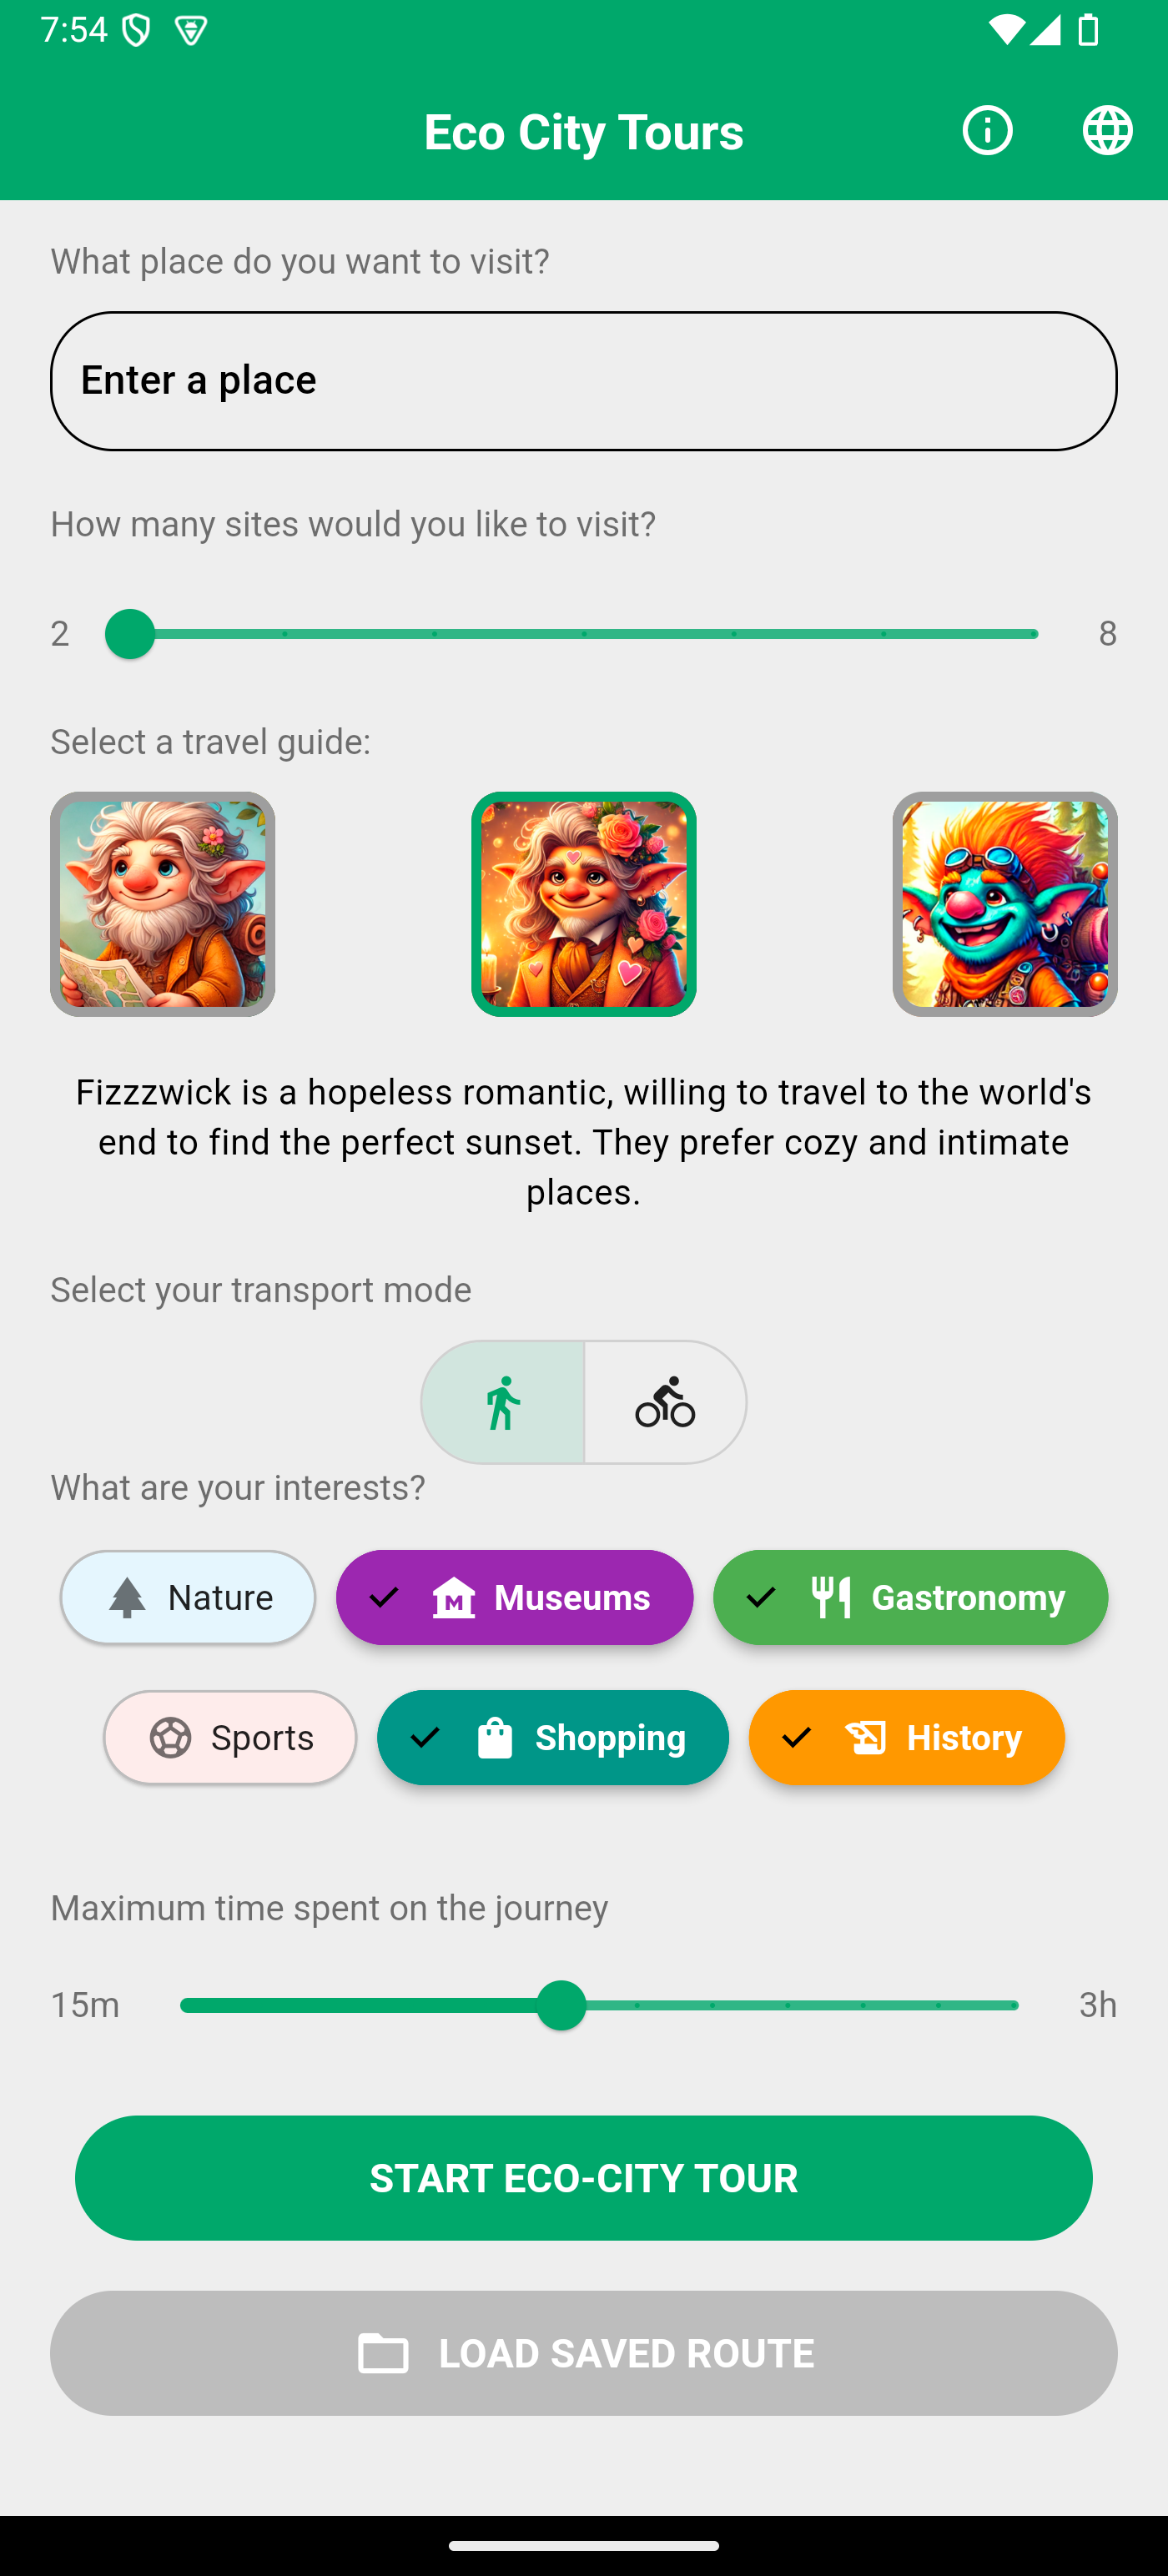
\includegraphics[width=0.4\linewidth]{E2-selection-tour-screen} 	
		\label{fig:selectionTourScreen}
		\caption{Pantalla de configuración de Eco City Tour}
		
	\begin{flushleft}
		Una vez establecidos los permisos veremos la pantalla de configuración del Eco City Tour, donde seleccionaremos nuestras preferencias a la hora de diseñar un tour turístico ecológico por un lugar.
	\end{flushleft}
		\textbf{Pasos a seguir:}
		\begin{enumerate}
			\item En primer lugar introducir la ciudad o sitio que se quiera visitar. 
			\item Se seleccionará cuantos \acrlong{pdi} queremos visitar.
			\item Se seleccionará un asistente si lo deseamos entre las tres opciones disponibles.
			\item Se indicará si queremos hacer la ruta a pie o en bici.
			\item Se indicará nuestras preferencias o gustos a la hora de viajar.
			\item Se indicará un tiempo máximo de tiempo en desplazamientos
			\item Por último se pulsará el botón de \textbf{generar Eco City Tour}
		\end{enumerate}		
	


\end{figure}
\newpage
\subsection{Pantalla de navegación de mapa}
\begin{figure}[H]
	\centering

		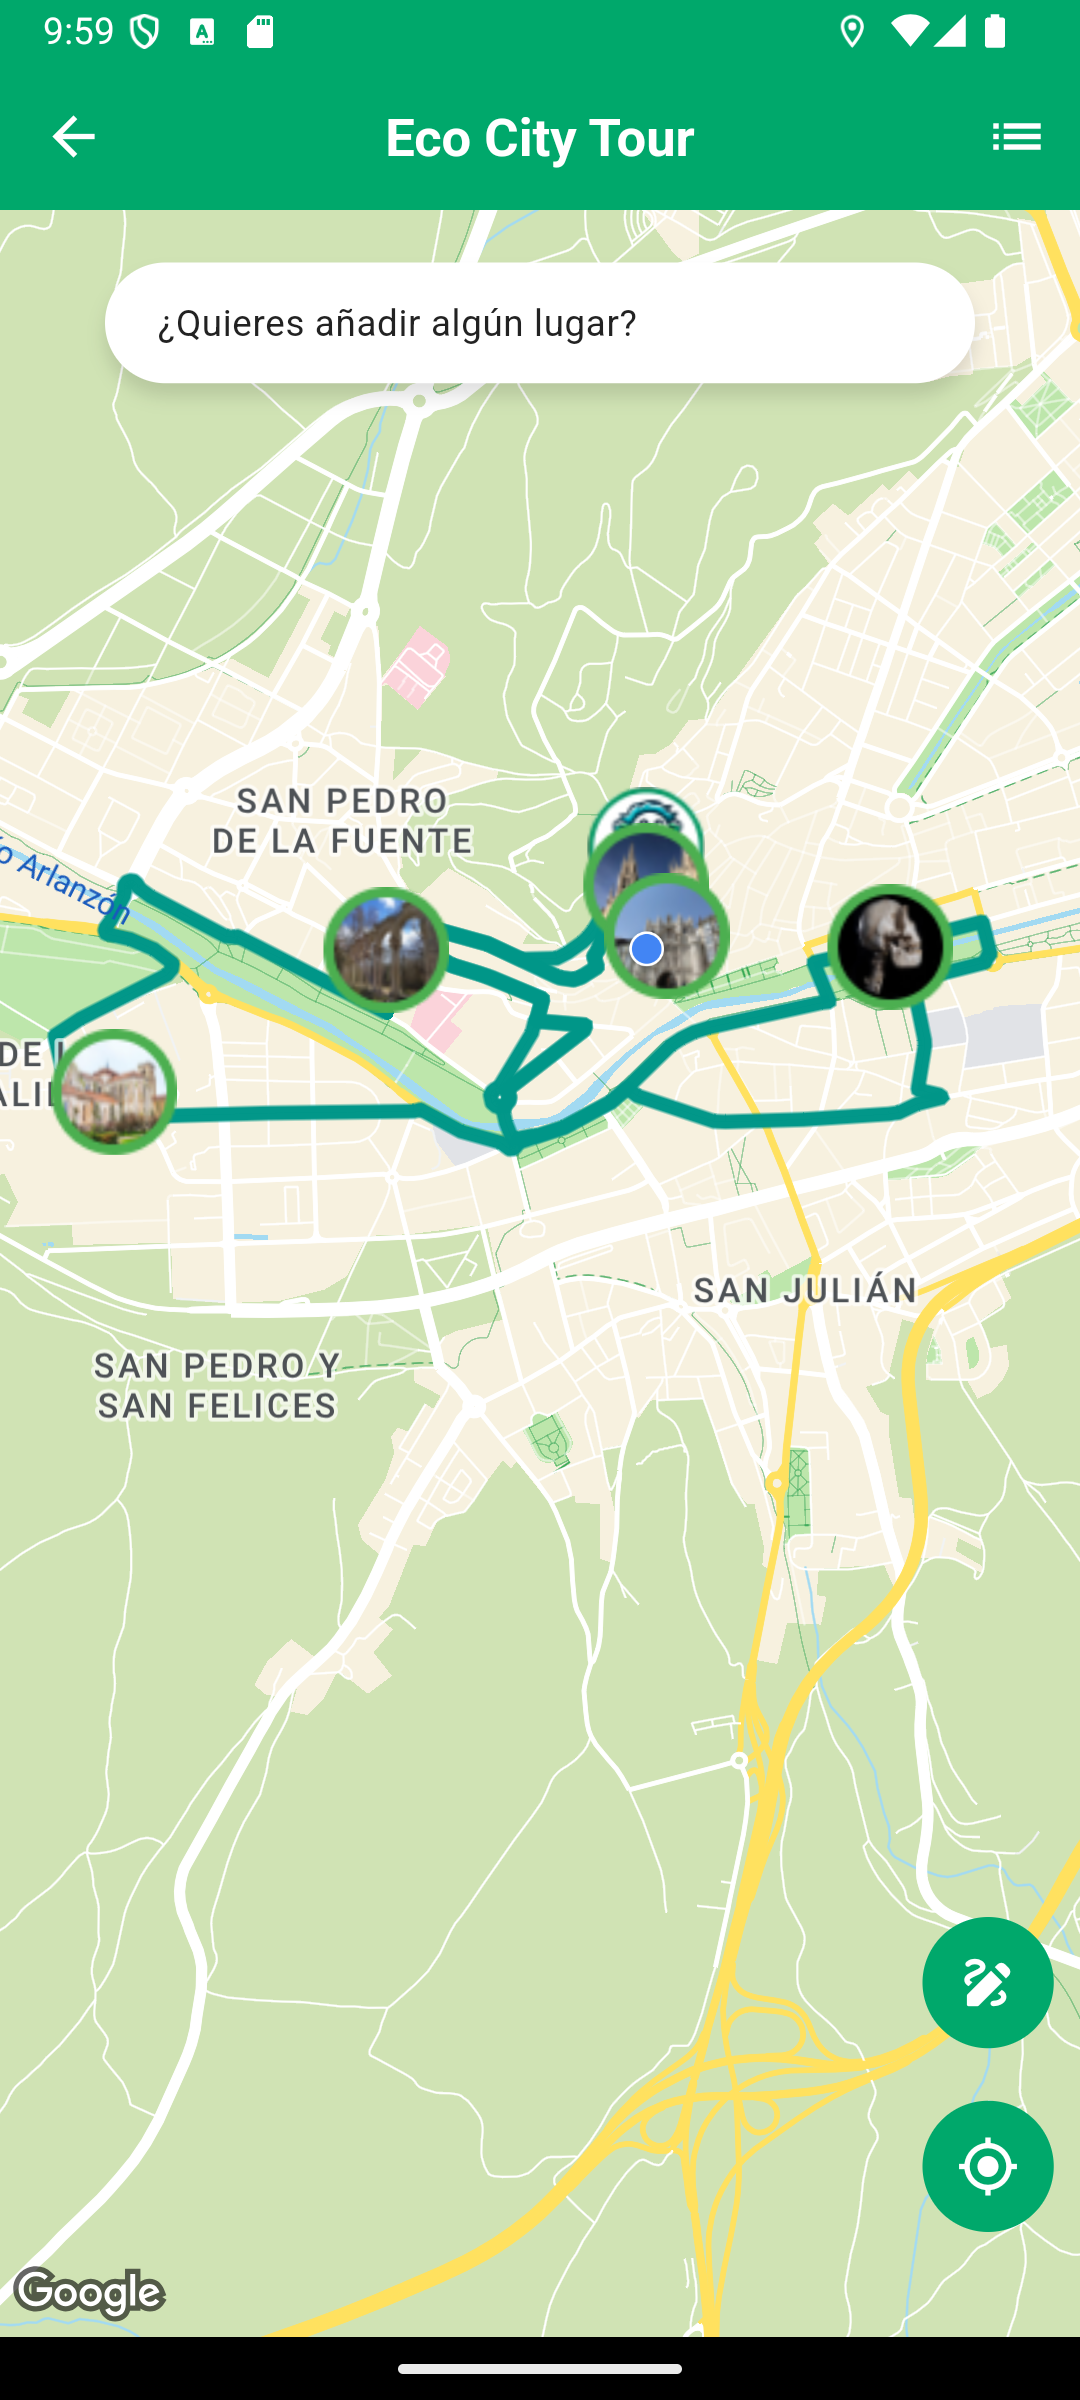
\includegraphics[width=0.4\linewidth]{E3-map-screen}
		\label{fig:navegacionMapa}
		\caption{Pantalla de navegación de mapa}
		
		Una vez cargado el tour podremos navegar por el mapa visualizando los distintos \acrshort{pdi} que la aplicación ha seleccionado para visitar, así como una ruta optimizada que une los puntos.
		
		\textbf{Desde aquí hay varias opciones:}
		\begin{itemize}
			\item Eliminar aquellos lugares que no queramos visitar.
			\item Añadir lugares a la ruta. Fig.~\ref{fig:busquedaPDI}
			\item Guardar el Eco City Tour. Fig.~\ref{fig:saveECT}
			\item Unir la posición GPS del usuario a la ruta. Fig.~\ref{fig:joinECT}
			\item Visualizar el seguimiento GPS del usuario. Fig.~\ref{fig:followingUser}
		\end{itemize}		
	
\end{figure}


\subsection{Buscar y añadir un \acrlong{pdi} al Eco City Tour}
\begin{figure}[H]
	\centering
	\begin{tabular}{m{0.4\textwidth} m{0.55\textwidth}}
		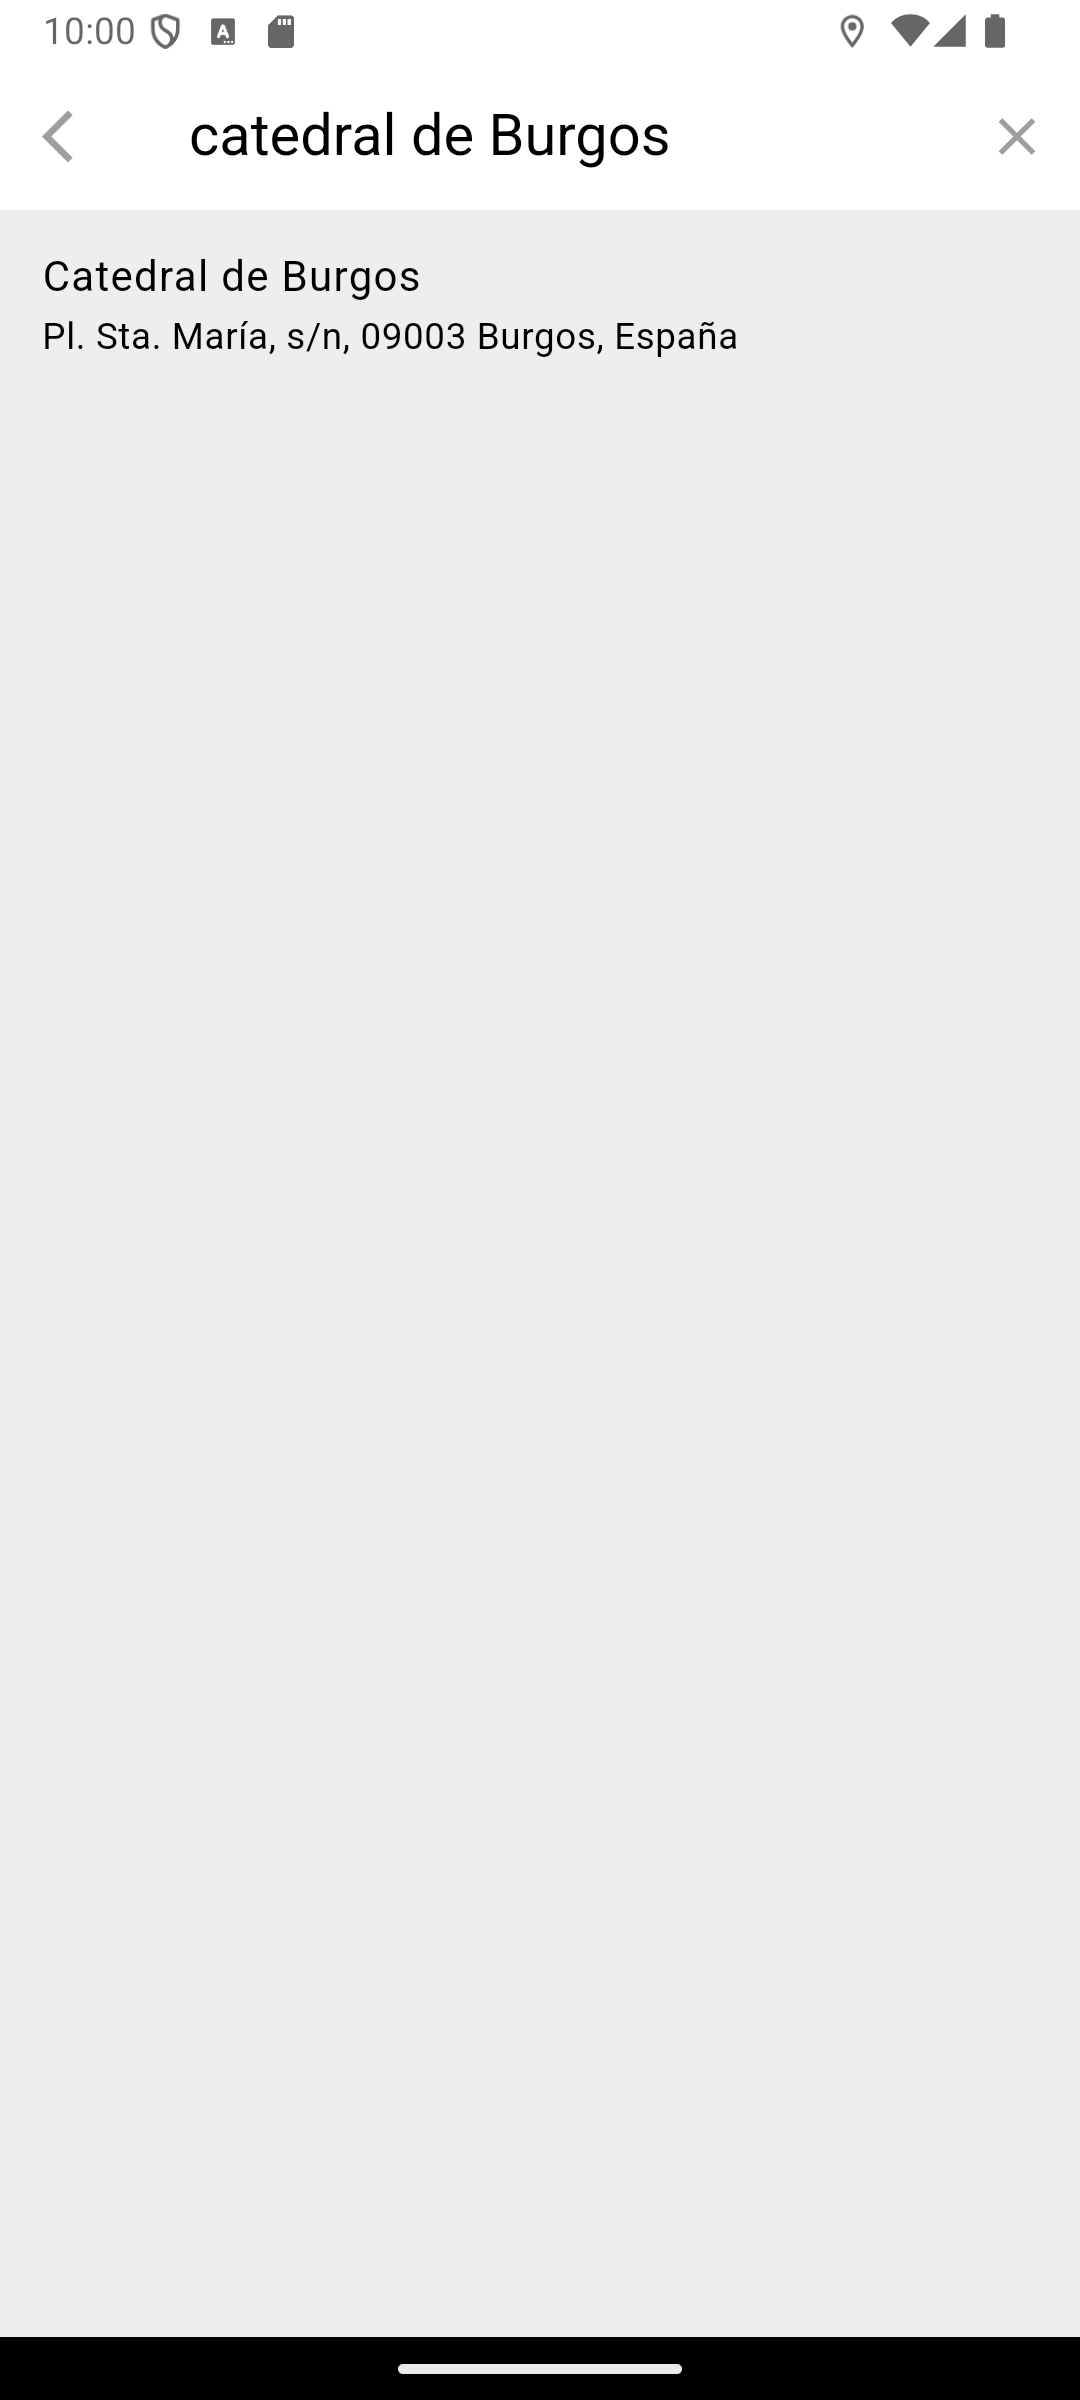
\includegraphics[width=0.6\linewidth]{E4-search-bar} & 
		\vspace{-10pt}
		Si el usuario conoce un lugar o desea añadir algún tipo de comercio (hospital, parque, supermercado) a la ruta solo tiene que seguir los pasos desde la Fig.~\ref{fig:navegacionMapa} 
		
		\textbf{Pasos a seguir:}
		\begin{enumerate}
			\item Introduce el nombre del lugar/lugares que quieras buscar en la barra de búsqueda. Por ejemplo en la Fig.~\ref{fig:busquedaPDI} se busca "Catedral de Burgos", mostrando un solo resultado 
			\item El usuario pulsará sobre el resultado que desea añadir.
			\item El sistema añade el lugar a la ruta y recalcula el camino más corto.
		\end{enumerate}		
	\end{tabular}
	\caption{Búsqueda de \acrshort{pdi}}
	\label{fig:busquedaPDI}
\end{figure}


\subsection{Conocer detalle de \acrshort{pdi}}
\begin{figure}[H]
	\centering
	\begin{tabular}{m{0.4\textwidth} m{0.55\textwidth}}
		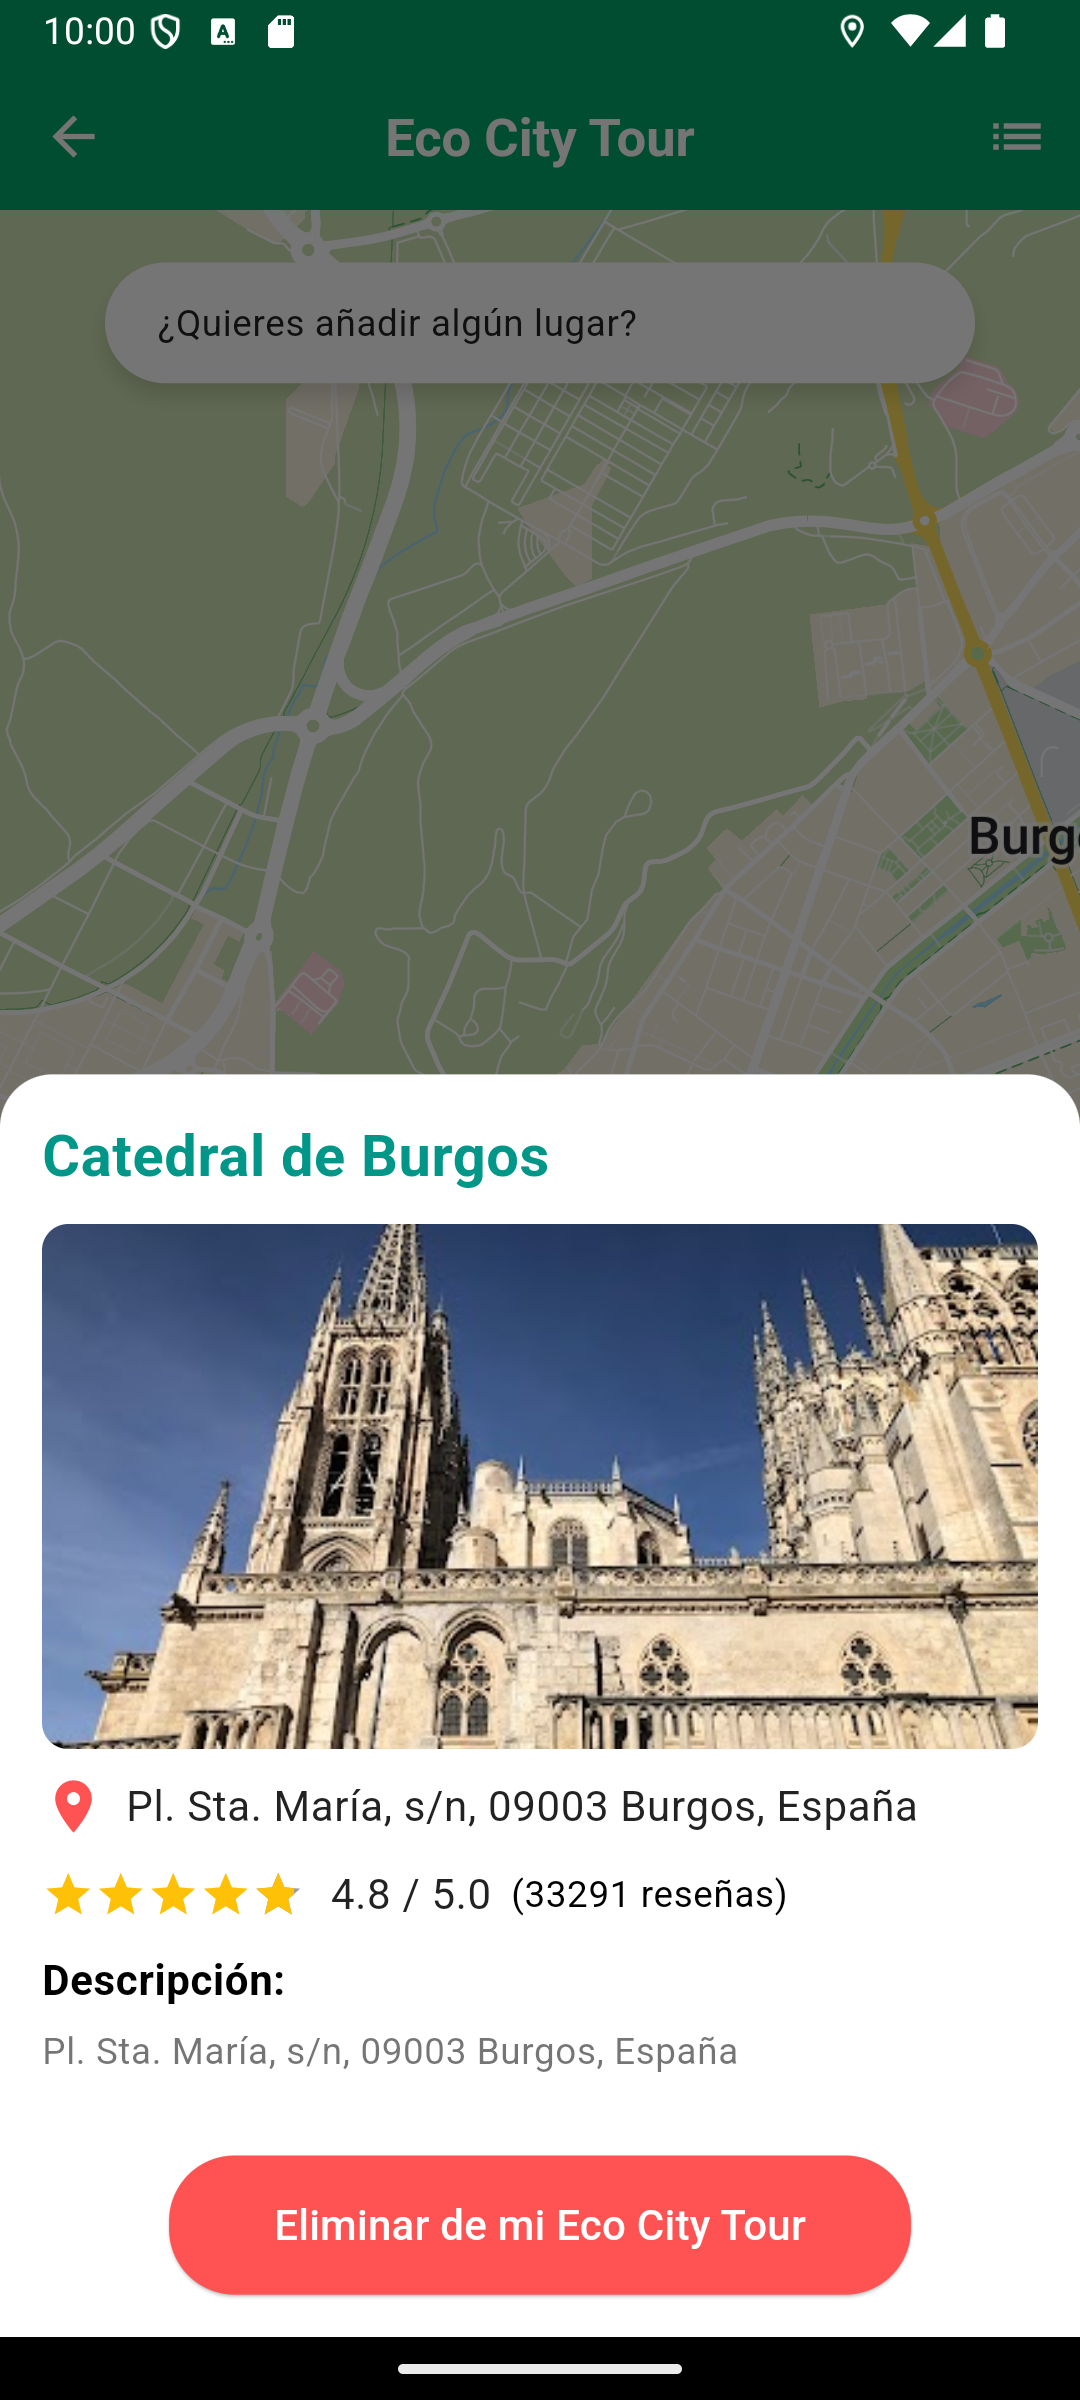
\includegraphics[width=0.6\linewidth]{E5-PDI-detalle} & 
		\vspace{-10pt}
		Uno de los elementos básicos de la navegación en el mapa que podemos ver en la Fig.~\ref{fig:navegacionMapa} es la de buscar información de un \acrlong{pdi} al seleccionar un elemento se nos muestra una imagen, una descripción, una valoración entre las obtenidas en Google y la opción de eliminar la visita del tour si no es de nuestro agrado. 
	\end{tabular}
	\caption{Detalle de \acrshort{pdi}}
	\label{fig:detallePDI}
\end{figure}

\subsection{Resumen de Eco City Tour creado}
\begin{figure}[H]
	\centering
	\begin{tabular}{m{0.4\textwidth} m{0.55\textwidth}}
		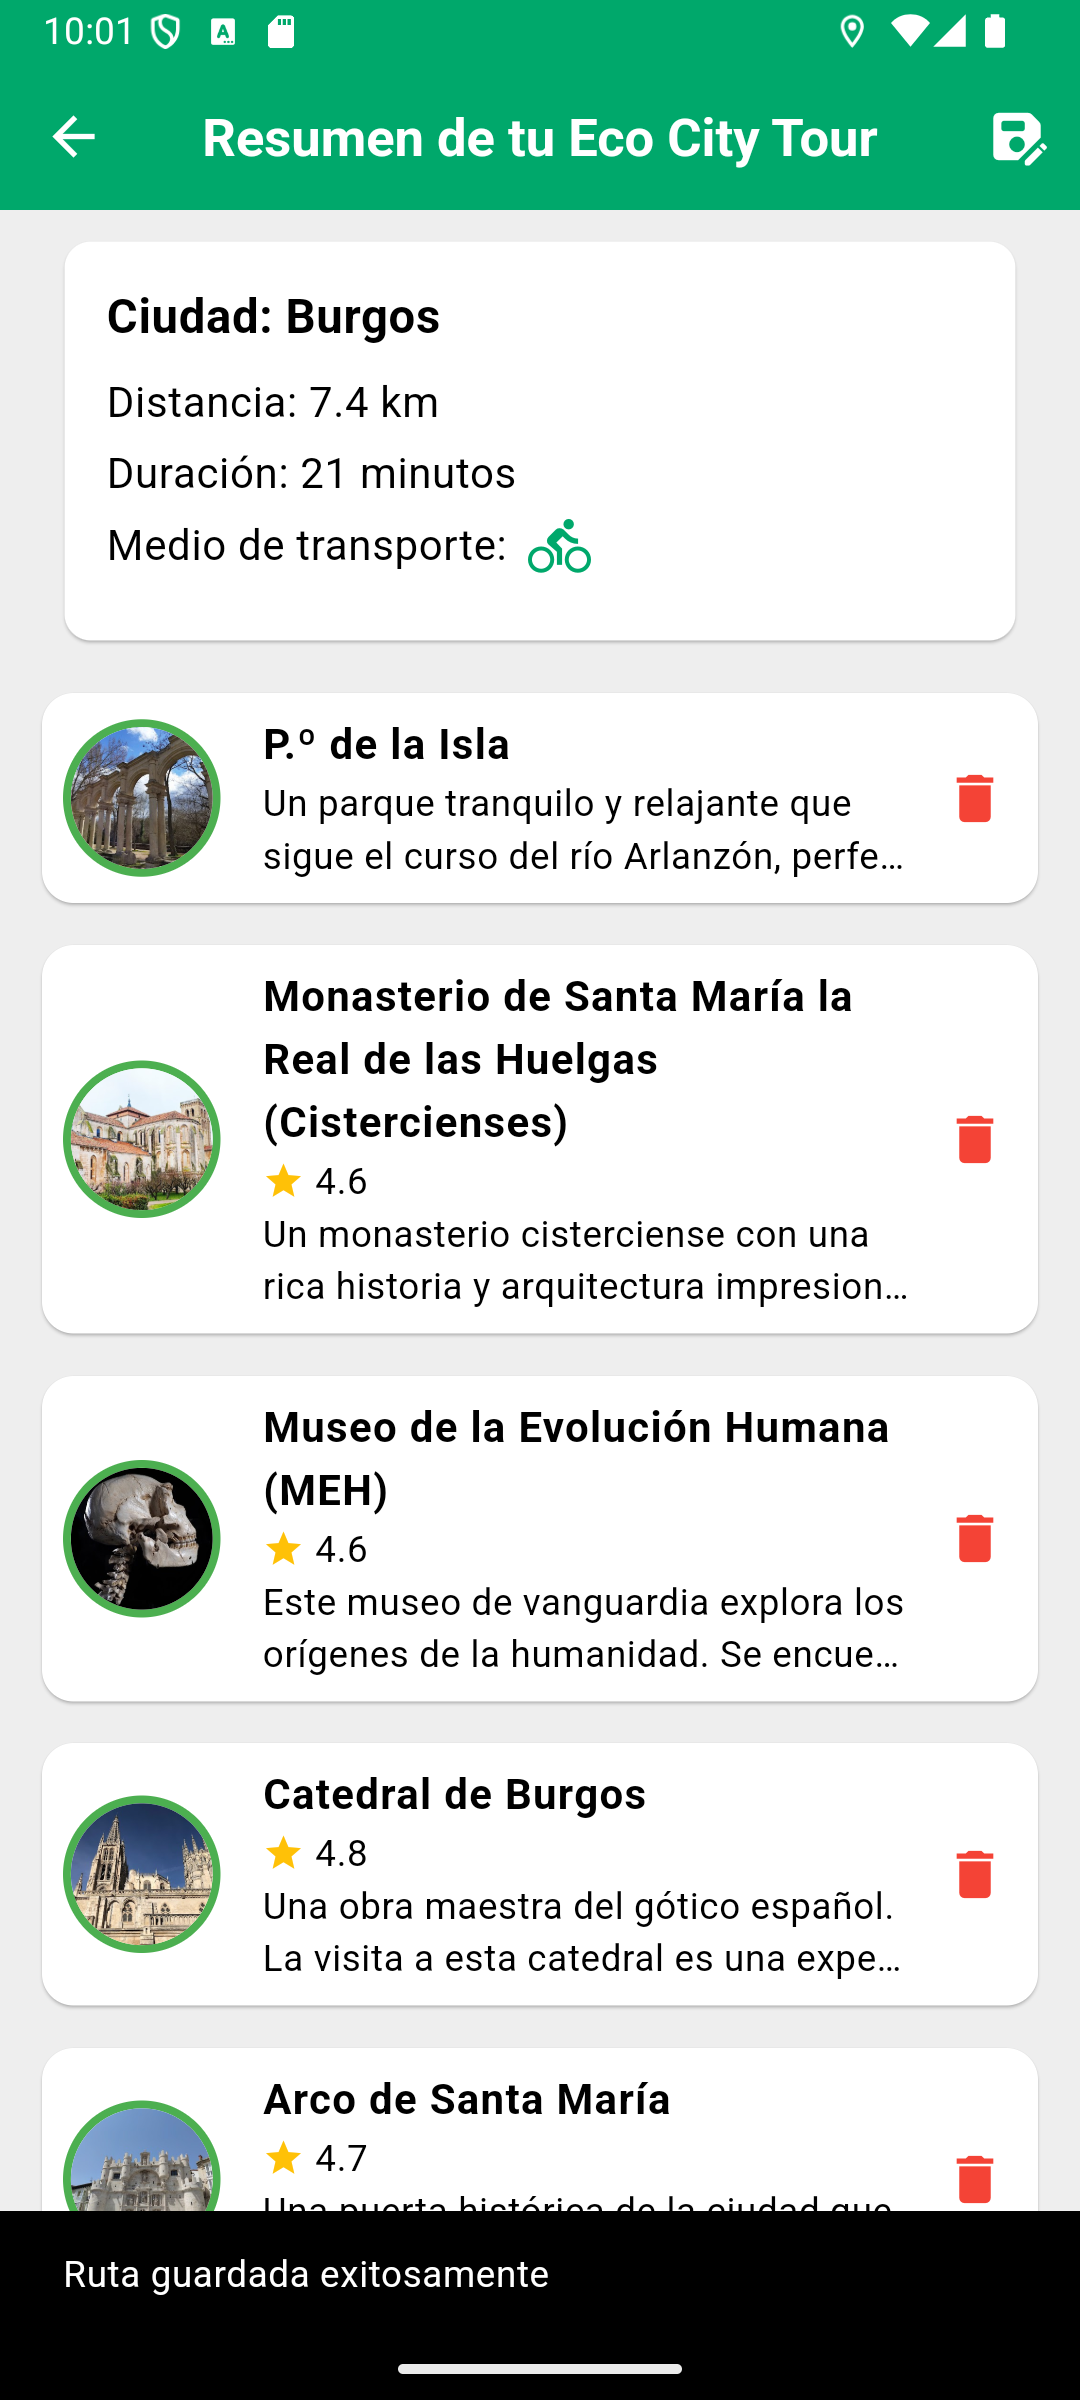
\includegraphics[width=0.6\linewidth]{E6-summary-screen} & 
		\vspace{-10pt}
		Desde el mapa podemos acceder a esta ventana que nos mostrará en su parte superior un resumen de las características del tour y en la parte inferior cada uno de los \acrlong{pdi} que forman el Eco City Tour.
		
		\textbf{Opciones:}
		\begin{enumerate}
			\item Podemos ampliar la información de la descripción.
			\item Eliminar del Eco City Tour un \acrshort{pdi}
			\item Guardar el Eco City Tour actual (Fig.~\ref{fig:saveECT}) o volver al mapa (Fig.~\ref{fig:navegacionMapa})
		\end{enumerate}		
	\end{tabular}
	\caption{Pantalla de resumen del Eco City Tour}
	\label{fig:resumenECT}
\end{figure}

\subsection{Guardar Eco City Tour}
\begin{figure}[H]
	\centering
	\begin{tabular}{m{0.4\textwidth} m{0.55\textwidth}}
		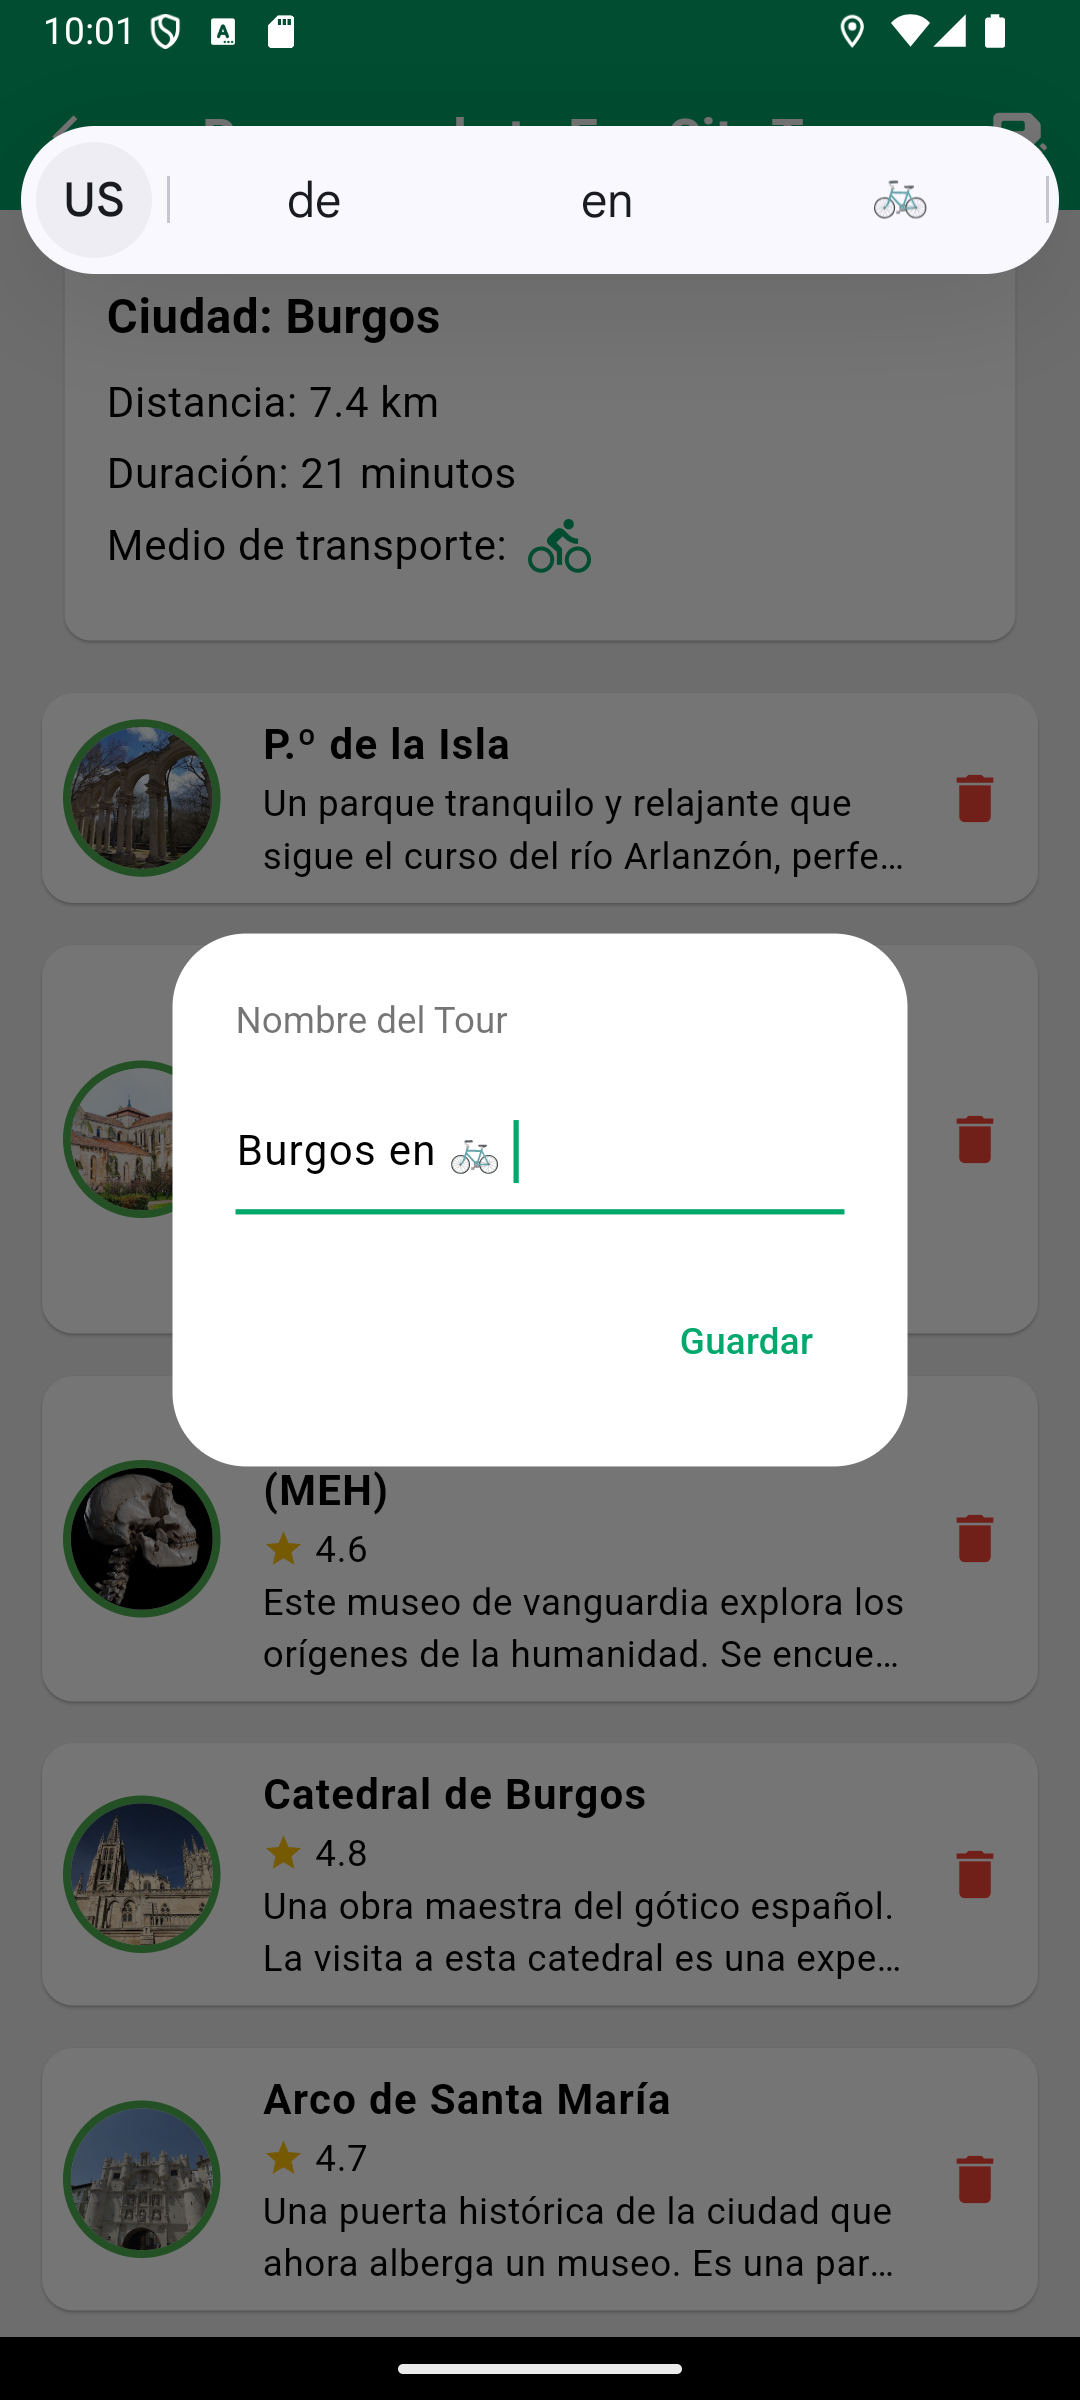
\includegraphics[width=0.6\linewidth]{E7-save-tour} & 
		\vspace{-10pt}
		Si queremos guardar la ruta para verla en otra ocasión el usuario puede guardar la información.
		\textbf{Pasos a seguir:}
		\begin{enumerate}
			\item Desde la pantalla de resumen del Eco City Tour, pulsar el botón de guardado de ruta.
			\item Elegimos un nombre.
			\item Un mensaje en la parte inferior nos informará que el Eco City Tour ha sido guardado con éxito.
		\end{enumerate}		
	\end{tabular}
	\caption{Pantalla de guardado del Eco City Tour}
	\label{fig:saveECT}
\end{figure}

\subsection{Cargar Eco City Tour}
\begin{figure}[H]
	\centering
	\begin{tabular}{m{0.4\textwidth} m{0.55\textwidth}}
		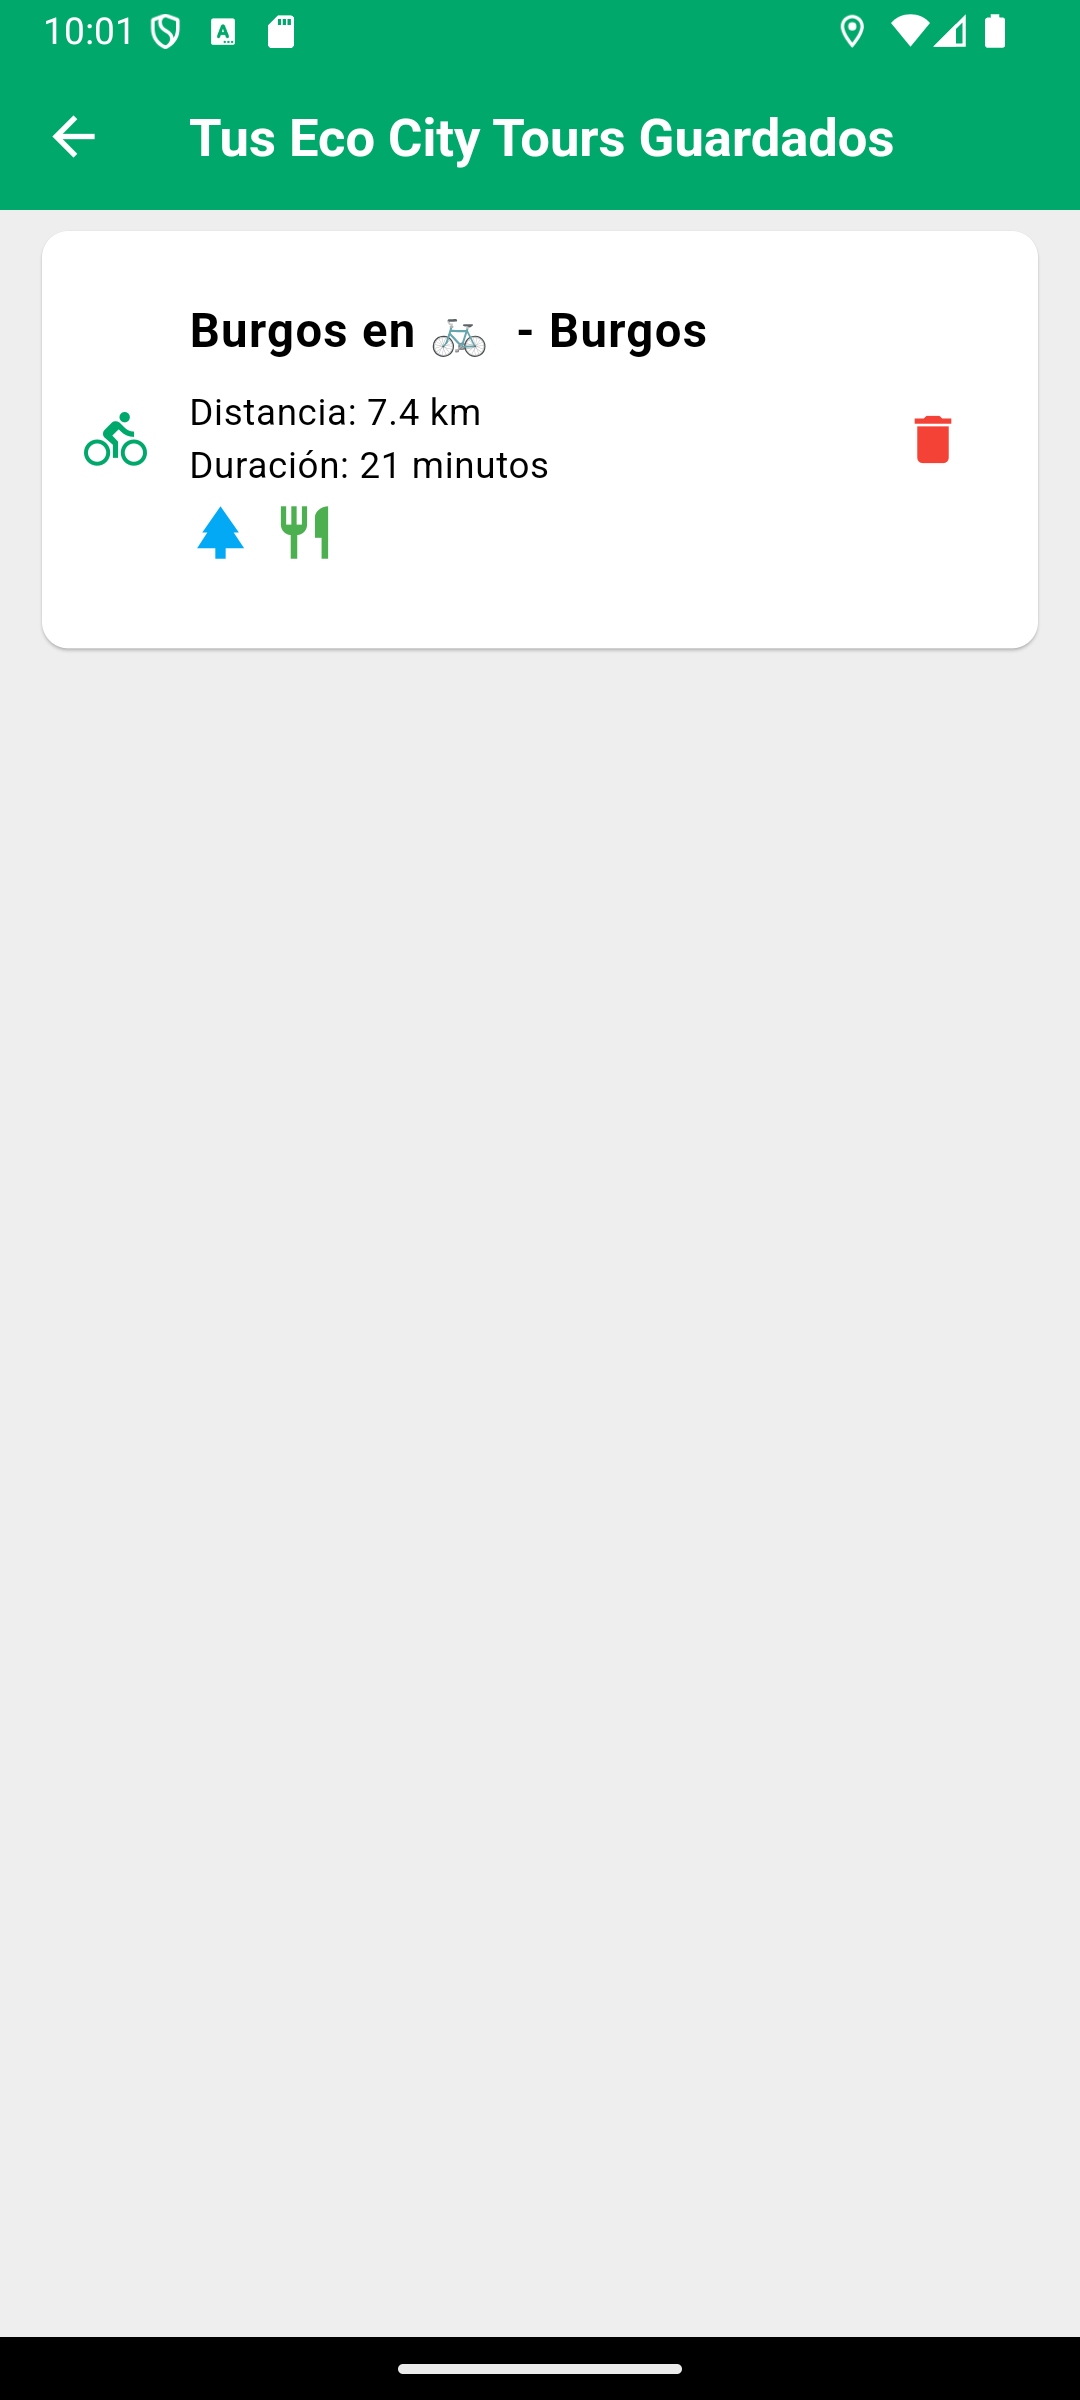
\includegraphics[width=0.6\linewidth]{E8-load-tour} & 
		\vspace{-10pt}
		Desde la pantalla de configuración (Figura~\ref{fig:selectionTourScreen}) podemos ver todos nuestras rutas personales guardadas.
		Simplemente seleccionaremos sobre el Eco City Tour que queramos cargar sobre el mapa y la pantalla de navegación del mapa  (Fig.~\ref{fig:navegacionMapa}) se mostrará en el mapa con el Eco City Tour guardado, mostrando la información relevante y todos los \acrlong{pdi}.	
	\end{tabular}
	\caption{Pantalla de carga del Eco City Tour}
	\label{fig:loadECT}
\end{figure}

\subsection{Unirse al Eco City Tour}
\begin{figure}[H]
	\centering
	\begin{tabular}{m{0.4\textwidth} m{0.55\textwidth}}
		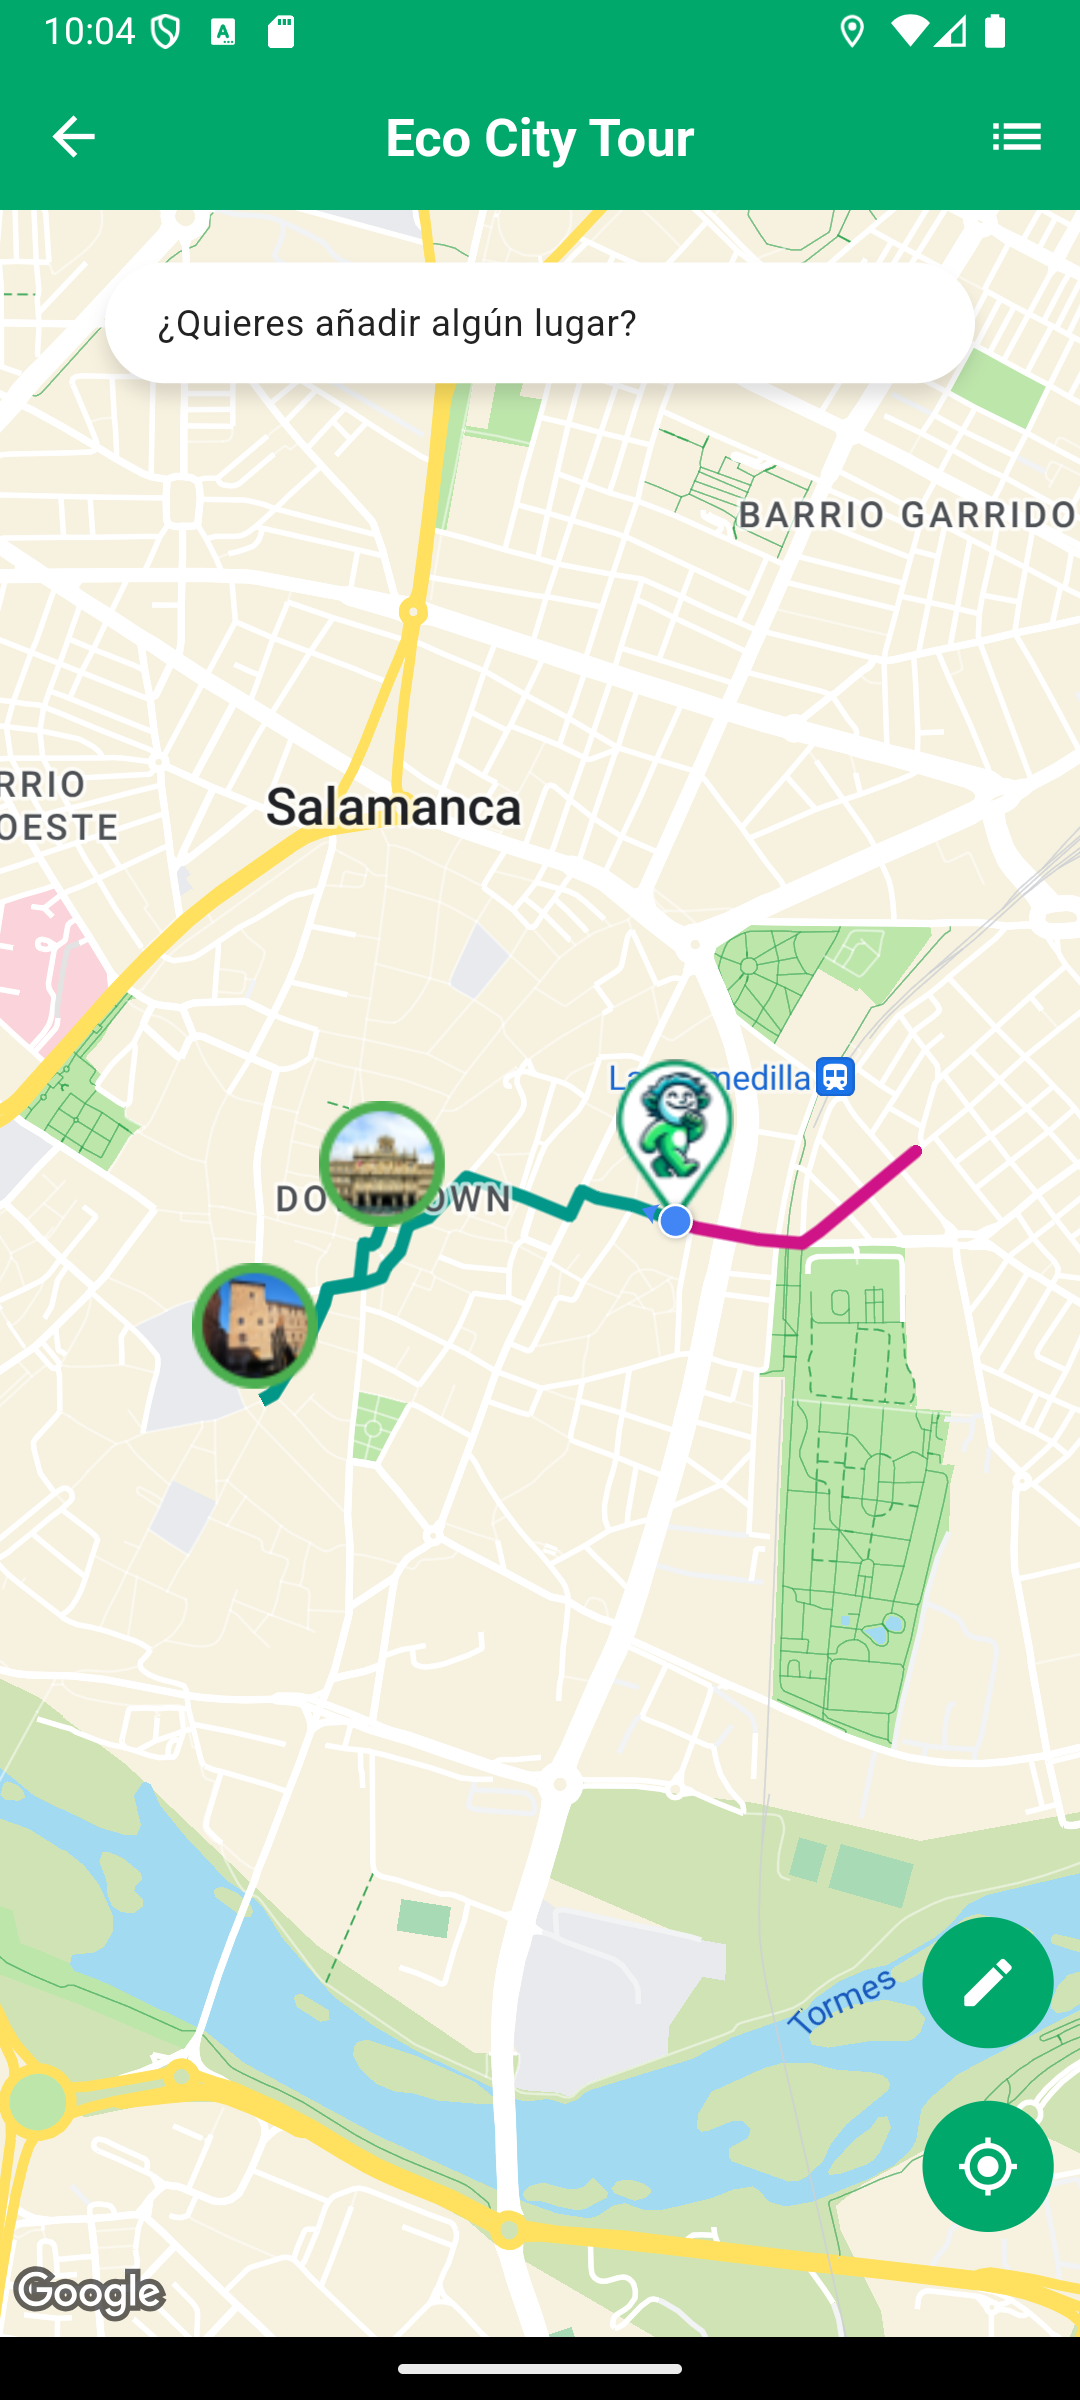
\includegraphics[width=0.6\linewidth]{E10-join-tour} & 
		\vspace{-10pt}
		Precisamente si el usuario está en un sitio clave que no quiere perder o simplemente quiere que la ubicación forme parte del Eco City Tour puede pulsar el botón inferior de la pantalla del mapa (Fig.~\ref{fig:navegacionMapa}) y se añadirá un nuevo \acrshort{pdi} con la ubicación del usuario y se recalculará de nuevo la ruta más corta entre los puntos que estaban creados y la posición del usuario.
		
		Como si de un \acrlong{pdi} corriente se tratase se puede eliminar en cualquier momento.
	\end{tabular}
	\caption{Unirse al Eco City Tour}
	\label{fig:joinECT}
\end{figure}

\subsection{Seguimiento en vivo de la posición del usuario}
\begin{figure}[H]
	\centering
	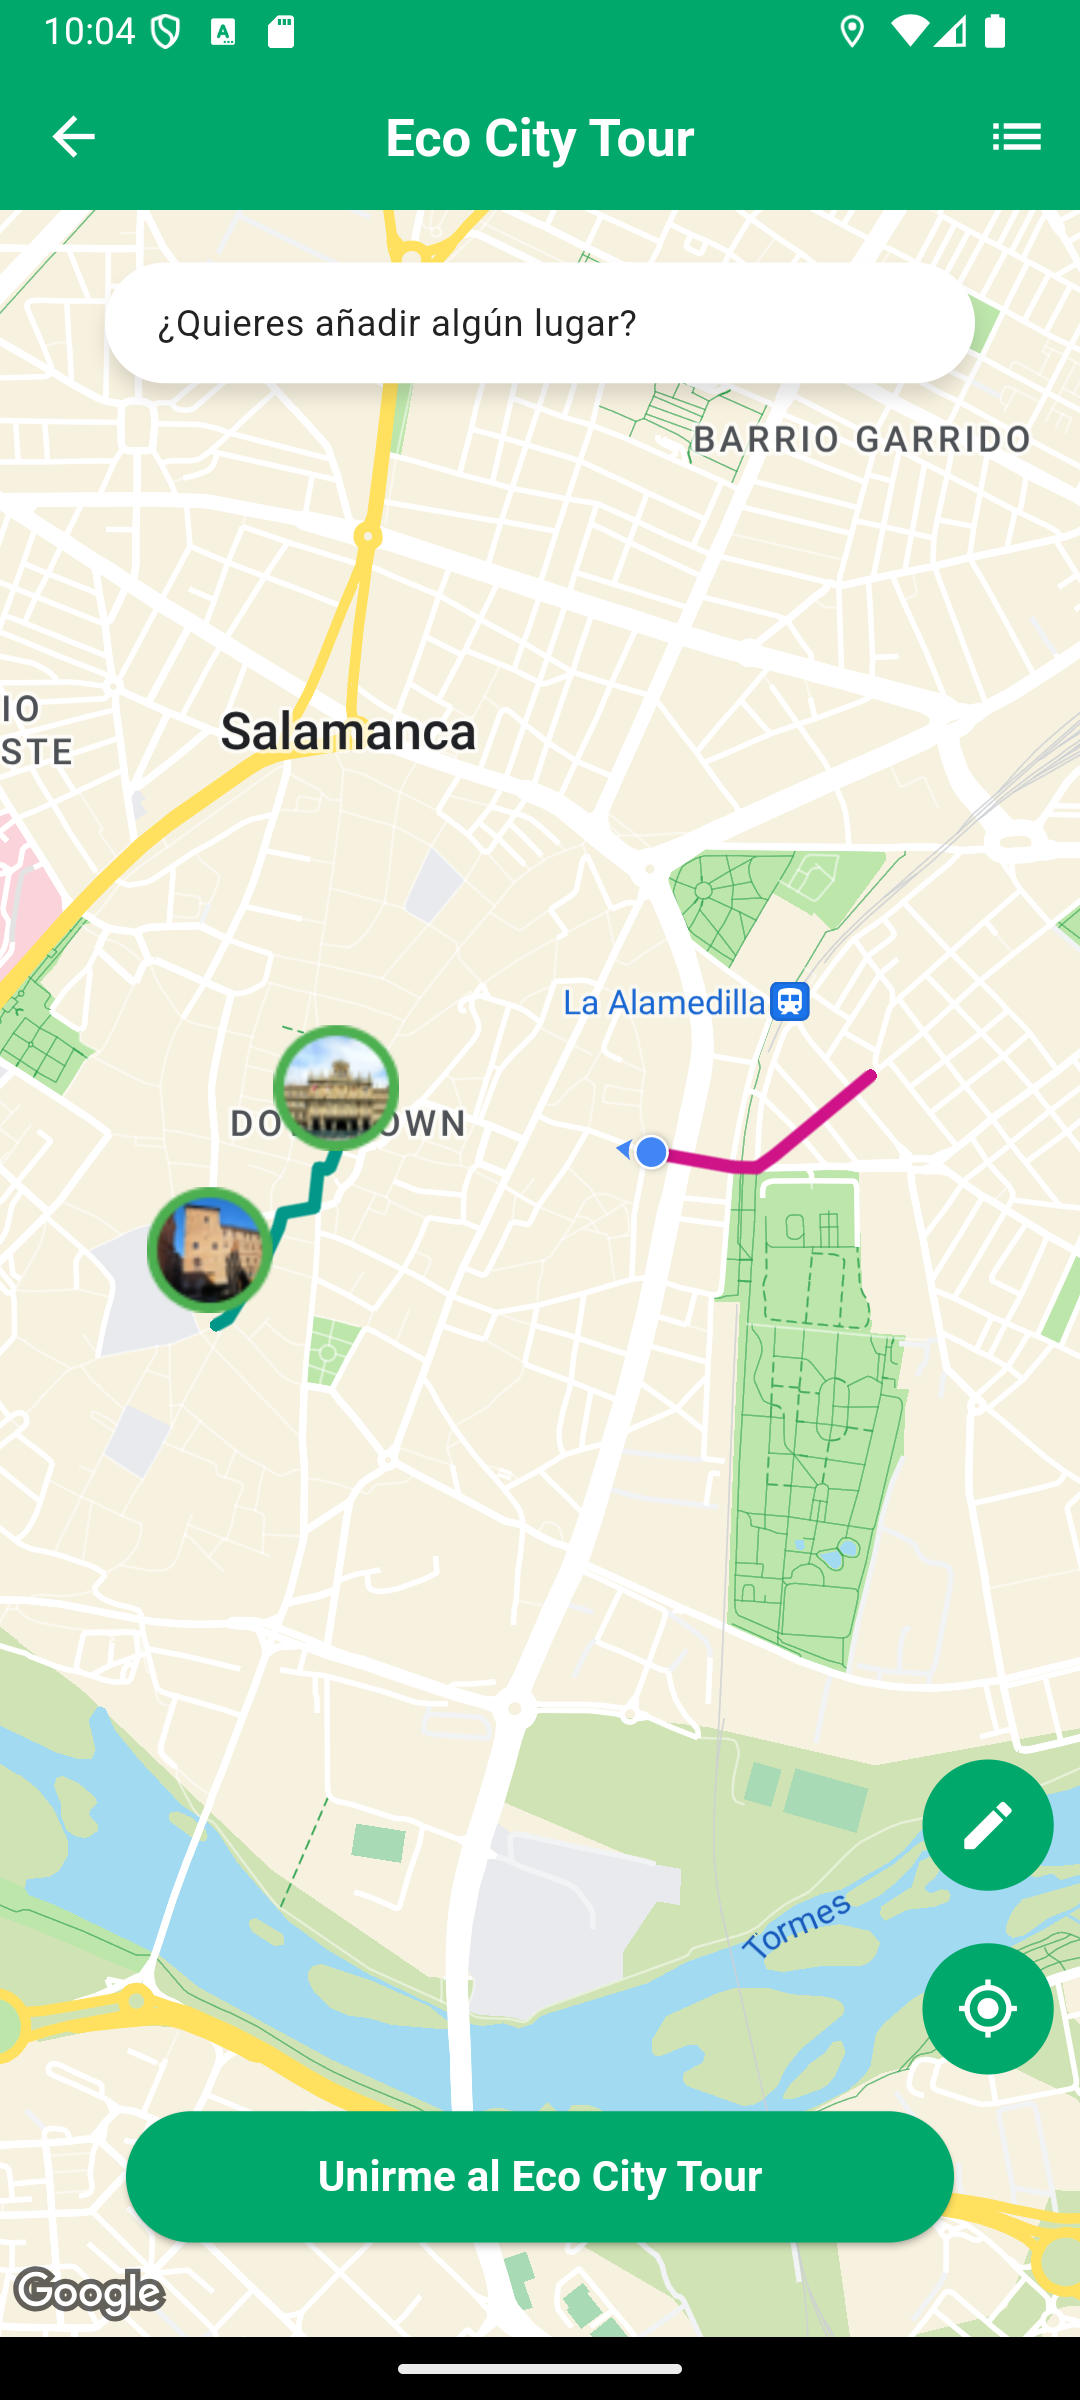
\includegraphics[width=0.35\linewidth]{E9-following-user} 
	\caption{Seguimiento en vivo de la posición del usuario}
	\label{fig:followingUser}
	\vspace{-10pt}
\end{figure}

Otras opciones que se pueden llevar a cabo desde la pantalla de navegación del mapa (Fig.~\ref{fig:navegacionMapa}) las llevamos a cabo con los botones flotantes inferiores, tenemos los dos siguientes:
		
\begin{enumerate}
	\item Permite que se muestre sobre pantalla un seguimiento del usuario, el camino que ha seguido se mostrará en el mapa y podrá comprobar su recorrido en todo momento. Para desactivar la línea solo tenemos que pulsar de nuevo el mismo botón.
	\item El segundo botón centrará la pantalla del mapa sobre la ubicación actual del dispositivo y permanecerá así hasta que se mueva de nuevo la pantalla.
\end{enumerate}		

Estas opciones amplían la funcionalidad de un turista, permitiendo controlar en todo momento su recorrido.







\apendice{Anexo de sostenibilización curricular}

\section{F.1. Introducción}
Durante el desarrollo del Trabajo Final de Carrera, he utilizado e implementado las disciplinas de la sostenibilidad en el diseño de una aplicación móvil. Ha sido de hecho un gran reto el tratar de generar rutas turísticas de tal manera que promocionen la sostenibilidad. Al final la solución presentada cumple con el \acrfull{ods11} fomentando principalmente la sostenibilidad de ciudades y los asentamientos humanos.

El valor principal de este \acrfull{ods}, como ya se ha tratado, radica en su papel de facilitador en la medida que, al resolver de manera integral y transversal todas las cuestiones relacionadas con la sostenibilidad de las ciudades, tiene un efecto secundario positivo en los demás \acrshort{ods}.

\section{Competencias de Sostenibilidad Adquiridas}
A lo largo del trabajo de este proyecto, he seleccionado y elaborado las competencias de sostenibilidad en las siguientes áreas:
	
	\subsection{Contextualización Crítica del Conocimiento}
	Puedo contextualizar el conocimiento adquirido y relacionarlo críticamente con los desafíos globales y locales en las áreas sociales, económicas y ambientales tan influenciadas por el turismo sostenible.
		
	\subsection{Uso Sostenible de Recursos}
	El desarrollo de la aplicación se enfocó en la utilización sostenible de los recursos. Traté de aplicar la eficiencia en el desarrollo de software al usar tecnologías que consumen la menor energía posible y al priorizar el uso de herramientas open-source, siempre que me fue posible.
		
	\subsection{Participación en Procesos Comunitarios}
	El desarrollo de esta aplicación exige una comprensión en profundidad de los procesos comunitarios. Se ha llevado a cabo por ejemplo al decir que no solo los turistas se benefician de su uso, sino que las rutas turísticas también promueven la movilidad sostenible y mejoran el bienestar de la comunidad local.
			
	\subsection{Principios Éticos y Valores de Sostenibilidad}
	 He incorporado prácticas éticas y valores de sostenibilidad en todo el trabajo descartando por ejemplo aquellas modificaciones que pudieran dar como resultado un conflicto entre la comunidad local y la turística.
				
\section{Aplicación de Competencias en el Proyecto}
				
Se utilizaron las siguientes competencias aprendidas en el desarrollo del proyecto:
	\subsection{Diseño y Funcionalidad de la Aplicación}
						
	El diseño de la aplicación ha seguido un enfoque centrado en el usuario cuyo propósito era diseñar una solución intuitiva, fácil de usar que promueva la movilidad sostenible: con ciclistas o peatones que disfruten de un viaje personalizado, uniendo los \acrfull{pdi} de una manera eficiente usando planificadores de rutas optimizados a tal efecto.
						
	\subsection{Impacto Social y Ambiental}
	La realización del proyecto busca no solo ser ventajosa para los turistas, sino que también reduce las emisiones de carbono al tiempo que permite a los miembros de la comunidad contribuir a la sostenibilidad de dicha ciudad en su conjunto.
							
	\subsection{Educación y Conciencia ambiental}
	El proyecto informará a los ciudadanos no solo con datos de rutas turísticas específicas, sino también buscará sensibilizar acerca de la movilidad sostenible y los beneficios ambientales que provienen de los dilemas referentes al transporte en los que participan.
								
\section {Conclusión}
Este Trabajo ha sido una experiencia informativa y esclarecedora para mí, tal y como indica en el artículo \cite{markiegi}, trabajar en el desarrollo de una aplicación que pone en práctica soluciones que favorecen los ODS te hace más consciente de los múltiples factores que impiden su cumplimiento. Este tiempo me ha dotado del enfoque que se necesita para enfrentar, de manera consciente y sostenible, los desafíos actuales y futuros con una visión global que trabaje activamente hacia un desarrollo sostenible y me siento capaz de liderar nuevas soluciones tecnológicas que potencien los ODS.



\printnoidxglossary[type=\acronymtype]
\printnoidxglossary[]

\bibliographystyle{plain}
\bibliography{bibliografiaAnexos}

\end{document}
